\documentclass[11pt,letterpaper]{article}% insert '[draft]' option to show overfull boxes
%
\usepackage{amsmath,amsbsy,amsfonts,amssymb}
\usepackage{varioref}%  smart page, figure, table, and equation referencing
\usepackage{wrapfig}%   wrap figures/tables in text (i.e., Di Vinci style)
\usepackage{graphicx}
\usepackage{amsmath}
\usepackage{algpseudocode}
\usepackage{color}
%\usepackage{hyperref}
\usepackage{threeparttable}% tables with footnotes
\usepackage{dcolumn}%   decimal-aligned tabular math columns
  \newcolumntype{d}{D{.}{.}{-1}}
  \usepackage{glossaries}
 \usepackage{nomencl}%   nomenclature generation via makeindex %******************************************
  \makeglossaries %*************************************************************************
 \usepackage{subfigure}% subcaptions for subfigures
 \usepackage{subfigmat}% matrices of similar subfigures, aka small mulitples
 \usepackage{fancyvrb}%  extended verbatim environments
  \fvset{fontsize=\footnotesize,xleftmargin=2em}
 \usepackage{lettrine}%  dropped capital letter at beginning of paragraph
 \usepackage[dvips]{dropping}% alternative dropped capital package
 \usepackage[colorlinks]{hyperref}%  hyperlinks [must be loaded after dropping]
%\topmargin -0.5 in \oddsidemargin 0.1 in \textheight 9.25 in
\topmargin -0.3 in \oddsidemargin 0.1 in \textwidth 6.6 in
\textheight 8.4 in
\title{Targeted Delivery of Acoustic Energy for Self-Healing}
\author{ Brian C. Fehrman, Umesh A. Korde\footnote{E-mail: Umesh.Korde@sdsmt.edu, Phone: 1-(605)355--3731}\\
Department of Mechanical Engineering\\
South Dakota School of Mines and Technology\\
501 East St. Joseph Street, Rapid City, SD 57701, USA\\
}

\begin{document}%
\maketitle
%\begin{abstract}
\baselineskip 18 pt
\section*{ABSTRACT}
Self healing materials capable of autonomic crack healing are
potentially important in space and terrestrial applications. Where
damage-causing forces and healing forces compete, it is of
interest to consider ways to increase the healing rate. This paper
investigates the use of acoustic energy for this purpose. As a
means for targeted acoustic energy delivery to the crack site, we
study time reversal mirrors (iterative time reversal and playback)
for stress wave focusing at a discontinuity.

The paper begins with a discussion of the key analytical results.
Both pulse propagation and eigenfrequency vibrations are analyzed,
and it is argued that if sufficient time is allowed between
successive time reversed playbacks, the focused pulse amplitude
grows faster than the eigenfrequency vibrations. Experimental implementations
of iterative time reversed play back on solid circular steel and
nylon rods with artificially introduced discontinuities show that
even in the 1-dimensional propagation studies here, time reversal
mirrors produce satisfactory focusing for a multi-tone pulse.
Based on the significant amplification seen in the steel rods and
the more dispersive and dissipative nylon rods, it appears that
acoustic energy could be delivered in a targeted manner to a crack
using iterative time reversal mirrors.


\vspace*{0.1 in} {submitted to: {\em J. Intelligent Material
Systems and Structures}}

%\end{abstract}
%*****************************************************************************
%nomenclature section here
%to generate nomenclature section
%run latex
%type in makeindex <filename>.glo -s nomencl.ist -o {filename}.gls     %*******left out the -o the first few times.
%run latex again

\newpage

\printglossary

\newpage

\section{INTRODUCTION}
\label{sect:intro}

Space structures on longer missions are exposed to a number of
challenges, including possible frequent collisions with
micrometeoroids and space debris.  Such impacts may threaten
functionality and shorten lifetimes in the case of lightweight
gossamer/membrane structures, and the damage may be impossible to
repair on orbit.  Structures using autonomic self-healing
materials would be attractive for such applications \cite{lee}.

A number of researchers around the world are engaged in the
development of self healing materials and many current
developments draw on biology \cite{sottos2010}.  Consideration of
self healing abilities of certain polymers and interest in
providing polymers with self healing properties dates back many
years, however, to the work of Wool and O'Connor \cite{wool}, who
discussed crack healing in epoxy polymers at elevated
temperatures.  Work has also been reported on crack healing in
thermoplastics through the introduction of a solvent and
application of heat \cite{wu}.  Room temperature healing of epoxy
polymers through chemical reactions was reported by White et al.
\cite{white}, who considered a material system with distributed
microcapsules (containing a reactive polymer and a catalyst),
which ruptured on crack arrival and facilitated a reaction across
the crack to restore the original structural properties.  Use of
solvents to heal cracks in epoxy thermosets at room temperature
was reported by Caruso et al. \cite{caruso}. A number of other
authors have also reported progress on the development of
autonomic self healing materials [e.g. Refs. \cite{sheng},
\cite{imperiale}].

One way to measure the effectiveness of an approach is to use the
quantity `healing rate', defined as the rate at which the
mechanical properties of the structure are recovered. The healing
rate is important from a structural point of view, since in
applications where healing forces (rate) must compete with the
damage causing forces (rate at which damage occurs) (e.g.
lightweight space vehicles), an increase in healing rate could tip
the balance in favor of the healing process.  This in turn could
help restrict the net damage,  possibly preventing the loss of
functionality and lengthening the structure's life.  In this work,
we consider a possible approach to enhancing the healing rate in
certain materials.  To this end, we return to the analysis of Wool
and O'Connor, which shows that healing rate increases with
increasing temperature and, during surface approach and wetting,
with increasing local stress\footnote{As pointed out later in this
section, Wool and O'Connor define 5 stages in the case of crack
healing; namely, (a) surface rearrangement, (b) surface approach,
(c) wetting, (d) diffusion, and (e) randomization.}. We argue that
with the correct technique, energy could be delivered acoustically
just to the crack site to increase the temperature and the stress
across the crack faces. Analytical calculations based on the
Wool--O'Connor theory \cite{wool} showed that epoxy healing rate
increased with increased local pressure across the crack faces
\cite{barnes}, while experimental results on nylon specimens
correlating an acoustically caused temperature increase with the
crack fusion rate showed that in the presence of acoustic
excitation, the crack fusion rate increased \cite{sarrazin}.

To investigate these effects further, we consider in
this work how may acoustic energy be delivered so that increased stress and
temperature only occur locally at the crack/defect and not over a
larger/undamaged area of the structure (where their action could
even prove deleterious).  We investigate the technique of time reversed acoustics \cite{fink},
which uses acoustic transducers and can enable highly localized
acoustic energy focusing at an anomaly or discontinuity within a
structure. The process of time reversed focusing of acoustic waves has been
studied for many years now, since its early beginnings in ocean
acoustics in the 1960's \cite{parvulescu}. Interpreted in the
frequency domain, the technique is analogous to the phase
conjugation approach used in adaptive optics \cite{fink},
\cite{anderson}. Many applications of time reversed acoustics
have been developed in recent years by Fink et al. (e.g. see
\cite{fink}). Applications of interest to this work include
nondestructive evaluation and medical surgery. Focused energy at
a defect can be used to detect and characterize a structural
defect, or when large enough, to destroy kidney stones in medical
surgery applications \cite{fink}. Time reversed focusing of waves
in air or water has been reported by a number of authors (e.g.
Refs. \cite{fink}, \cite{thomas}]. Of relevance to this work is
wave propagation in solid media, where time reversal is
challenging to implement and analyze due to the fact that solids
can support 6 different internal wave components, in addition to
certain types of guided waves (including surface waves). Anderson
et al. \cite{anderson} considered time reversal analysis of
seismic waves for earthquake source characterization and nuclear
explosion monitoring. Saenger et al. reported time reversed
modeling for nondestructive evaluation of concrete
\cite{saenger}, while time reversed focusing of Lamb waves was
studied by Harley et al. for nondestructive evaluation and
structural health monitoring of pipelines \cite{harley}.
Coexistence of eigenfrequency vibrations with the pulse signals to
be focused is an important consideration in structures that can be
treated as finite in relation to the space-time scale of the
focusing problem. The effect of eigenfrequency vibrations on the
focusing process was investigated by Sutin et al. \cite{sutin} on
a doped glass slab structure.

This paper represents a step toward our ultimate goal of
investigating the effect of focused acoustic energy on defect
healing in polymer solids.  Time reversed focusing as implemented
here requires no {\em a priori} or inferred knowledge of the
defect location, which could be an advantage over other focusing
approaches.  For instance, it is not difficult to visualize a
plate-like structure with a number of piezoelectric transducers
distributed over it (see Figure \ref{explain}).  One of the
transducers periodically sends out a known pulse (e.g. Lamb wave)
which is diffracted and scattered by any defect/crack that may be
developing in the structure.  The pulse as diffracted from the
defect is received by all of the transducers.  The record at each
transducer is saved and played back in reverse time (once all
recording is complete at all transducers) with the desired
amplification.  The waveforms emanating from the transducers then
trace their individual paths back to the defect and arrive
contemporaneously to coalesce into a larger waveform at the
defect.  The process then repeats itself, with each successive
iteration increasing the magnitude of the coalesced signal,
leading to a highly localized and amplified energy pulse at the
defect/crack, which in turn leads to a localized increase in the
stress and temperature at the defect. This increase continues
until convergence is reached in the presence of material
dissipation.
\begin{figure}
\begin{center}
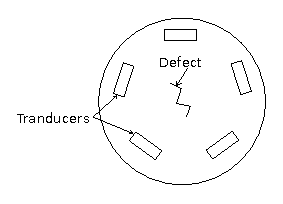
\includegraphics[width=9.7cm,height=7.75cm]{tr.eps}
\end{center}
% \vspace*{-20 pt}
 \caption[des1]
%>>>> use \label inside caption to get Fig. number with \ref{}
   { \label{explain}
Schematic showing the use of multiple transducers in a pulse-echo
mode causing focusing at a defect at an unknown point in the
plate.
 }
 \end{figure}
The initial interrogatory pulse is applied periodically, and
focusing results only when a crack or defect forms within the
region surrounded by the transducers (no time reversal and
playback occur when the signals received by the transducers
correspond to the transducer--transducer terms in the impulse
response function matrix for the transducer-plate system).  The
combined acoustic energy delivery--defect healing process can thus
be considered `semi-autonomic'.  Work has been reported on sonic
excitation (i.e. `sonication') to create `mechanophores' to be
mixed with the polymer to cause healing upon mechanical excitation
\cite{kryger}. In contrast, our work does not involve explicit
addition of  mechanophores, and is based on the Wool--O'Connor
theory relating greater stress/temperature to increased healing
rates.

%Focused energy delivery through time reversal mirrors is of vital
%to the present investigations.  Time reversed acoustic focusing
%has a long history, with the first implementations going as far
%back as 1962 \cite{parvulescu} in the context of ocean acoustics.
%Both analytically and practically it is often convenient to
%consider time reversal as phase conjugation in the frequency
%domain.

To facilitate greater insight, we consider here pure extensional
wave propagation in circular rods with known properties. Experience in iterative time reversal mirrors suggests that better
focusing is achieved in 2-dimensional wave propagation with
multiple transducers. For experimental convenience in the time reversal tests, we
study 1-dimensional propagation. Despite this, we find that time
reversed play back is still quite effective and produces
reasonable magnification and localization of energy.

The layout of the paper is as follows. Section \ref{sect:wav} discusses time-reversed focusing in
1-dimensional domains linking the piezoelectric excitation voltage
to the strain at the focused signal when it is caused at a
simulated defect. Section \ref{sect:vib} discusses the effect of
eigenfrequency vibrations, while section \ref{sect:calc} outlines
the calculations performed. Section \ref{sect:expt} discusses the time-reversed
focusing experiments on 1-dimensional circular rods. Results are
discussed in section \ref{sect:res}, and the main conclusions of
this paper are summarized in section \ref{sect:concl}.

\section{WAVE PROPAGATION ANALYSIS}
\label{sect:wav}

We investigate propagation and reversal in a circular rod of
finite length $L$ (the material is steel or nylon). The
propagating waveform is produced by one of the piezoceramic stack
transducers affixed at the rod ends (Figure \ref{tr_setup_1}). The transducers are constrained along their
longitudinal axes, have the same cross sectional area as the rod,
and are aligned with their longitudinal axes forming a straight
line with that of the rod.  A voltage pulse at the sending
transducer  A causes a stress variation to propagate in the
longitudinal direction $z$ with a magnitude related to the
$d_{33}$ piezoelectric strain constant. Because the diameter of
the transducer slightly exceeds the diameter of the rod, and the
strain variation over the rod's cross section is negligible, the
stress pulse propagating through the rod is also uniform over the
cross section.  Without any defects within the rod length, the
pulse simply propagates towards the receiving transducer B at the
opposite end. The impinging stress wave causes a voltage signal in
the receiving transducer, again with a magnitude related to the
$d_{33}$ strain constant. The following situation is considered in
this analysis:
\begin{itemize}
%\item Time reversed play back at transducer B such that the stress
%wave caused by the played back voltage combines with a new stress
%wave produced by transducer A at transducer A to produce an
%amplified waveform.
\item Suppose an internal planar defect occurs at an {\em a
priori} unknown location within the rod length. The pulse created
by transducer A reaches the defect plane and suffers a partial
reflection and partial transmission (see Figure \ref{tr_setup_1}).
The transmitted part travels to transducer B and produces a
voltage pulse at it. The reflected part travels back to transducer
A where it also creates a voltage pulse.  Both recorded voltage
signals are now time reversed and played back, with the stress
waves from these arriving at the defect simultaneously to produce
an amplified waveform.  This process is then repeated iteratively
until convergence.
\end{itemize}
The analysis below examines the effect of play back times, signal
phases and magnification on the overall amplification available
with the technique.  The reversed play back above will be repeated
multiple times in practice to produce iterative amplification
until convergence. For a finite-length rod, one must consider the
effect of natural or eigenfrequency vibrations set off within the
rod due to iterative pulse excitation at either end.  For
successful localized amplification based on this technique, the
natural transient vibration response of the rod should decay in a
time period shorter than the time window over which reversal is
performed.  This question is considered further in section
\ref{sect:vib}.  Finally, due to the relative complexity of
frequency-dependent dispersion, analysis/calculations are only
performed for non-dispersive propagation in a steel rod.  The case
of time reversal with dispersive propagation in nylon is only
studied experimentally.
%\footnote{This is achieved by introducing sufficient
%delay between successive iterations, as discussed in section
%\ref{sect:vib}.}.

The pulse propagates along the axis of the rod in the $z$
direction, and the deflection under it is denoted as $w(z,t)$.
The numerals 1, 2, and 3 as subscripts are associated with the $x,
y, z$ directions respectively. The constitutive relations
applicable to each sub-domain above are as follows:

\noindent {\bf{Sending transducer A}}: $0<z<l$

\begin{align}%
&T_3 = \overline{{C_{33}}}S_3 + \overline{d_{33}}D_3 \nonumber\\
&D_3 = \overline{{\varepsilon}^T_{33}}E_3 +
\frac{d_{33}}{s^E_{33}}S_3 \label{constitsend1}
\end{align}%
%
\nomenclature{$T_3$}{Stress in the $z$ direction; i.e. along the
longitudinal axis}%
\nomenclature{$S_3$}{Strain developed in the $z$ direction; i.e.,
along the longitudinal axis}%
\nomenclature{$C_{33}, C^\ast_{33}, C^c_{33}$}{Elastic constants
relating stress in $z$
direction to strain in $z$ direction (longitudinal axis): for transducer, rod material, `defect' respectively}%
\nomenclature{$D_3$}{Electric displacement in the z direction; i.e.,
charge density on a plane normal to the longitudinal axis}%
\nomenclature{$E_3$}{Electric field intensity in the $z$ direction}%
\nomenclature{$\varepsilon^T_{33}$}{Permittivity constant at
constant stress in the $z$
direction acting on field intensity in the $z$ direction}%
\nomenclature{$d_{33}$}{Piezoelectric strain constant relating
strain in $z$ direction to electric field intensity in the $z$
direction}%
\nomenclature{$s^E_{33}$}{Compliance constant at constant electric
field; reciprocal of
$C_{33}$}%
\nomenclature{$L$}{Length of steel or nylon rod}%
\nomenclature{$l$}{Length of piezoceramic transducers A and B}%
%\nomenclature{$V_c(t)$}{Voltage measurement at transducer A
%following time reversal}%
%
where
\begin{align}%
&\overline{C_{33}} =
\frac{1}{s^E_{33}\left(1-\frac{d^2_{33}}{s^E_{33}\varepsilon^T_{33}}\right)}
\nonumber\\
&\overline{d_{33}} =
-\frac{d_{33}/\varepsilon^T_{33}}{\left(1-\frac{d^2_{33}}{s^E_{33}\varepsilon^T_{33}}\right)}\nonumber\\
&\overline{\varepsilon_{33}} =
\frac{\varepsilon^T_{33}}{\left(1-\frac{d^2_{33}}{s^E_{33}\varepsilon^T_{33}}\right)}
\label{constinv1}
\end{align}
%

\noindent{\bf{Circular Rod}}: $l \leq z \leq L$
\begin{equation}
T_3 = C^\ast_{33}S_3 \label{constrod}
\end{equation}
%

\noindent{\bf{Receiving transducer B}}: $L < z \leq L+l$
\begin{align}
&T_3 = \overline{C_{33}}S_3 + \overline{d_{33}}D_3 \nonumber\\
&D_3 = \overline{\varepsilon_{33}}E_{33} + \frac{d_{33}}{s^E_{33}}
S_3 \label{constitrec1}
\end{align}
with the parameter definitions in equations (\ref{constinv1}).

The propagation of the pulse through the three bodies is described,
ignoring dissipation effects for the present, as%

\noindent{\bf{Sending transducer A}}: $0 \leq z \leq l$
\begin{equation}
\frac{\partial^2w}{\partial t^2} - c^2\frac{\partial^2w}{\partial
z^2} = 0 \label{proptrans1}
\end{equation}
\nomenclature{$c$}{Acoustic velocity in the piezoceramic transducer}%
\noindent{\bf{Circular rod}}: $l < z \leq L$
\begin{equation}
\frac{\partial^2w}{\partial t^2} -
{c^\ast}^2\frac{\partial^2w}{\partial z^2} = 0 \label{proprod1}
\end{equation}
\nomenclature{$c^\ast$}{Acoustic velocity in the rod material (steel or nylon); $=c_a$ for epoxy}%
\noindent{\bf{Receiving transducer B}}: $L < z \leq L+l$
\begin{equation}
\frac{\partial^2w}{\partial t^2} - c^2\frac{\partial^2w}{\partial
z^2} = 0 \label{proprec1}
\end{equation}
The boundary conditions at the interfaces are
\begin{equation}
w(l^{-},t) = w(l^{+},t) \label{bounddeftrans1}
\end{equation}
i.e., the deflection is continuous across the interface $z = l$.
In addition,
\begin{equation}
T_3(l^{-},t) = T_3(l^+,t) \label{boundstr1}
\end{equation}
i.e., the stress in the z direction is also continuous at the
interface $z = l$. Similar boundary conditions hold for $z = L+l$,
so that,
\begin{equation}
w(L+l^{-},t) = w(L+l^+,t) \label{bounddefrec2}
\end{equation}
and
\begin{equation}
T_3(L+l^{-},t) = T_3(L+l^+,t) \label{boundstr2}
\end{equation}
The electronic equivalent circuits for the sending and receiving
transducers are shown in Figure \ref{equiv_circ}.
\begin{figure}
\begin{center}
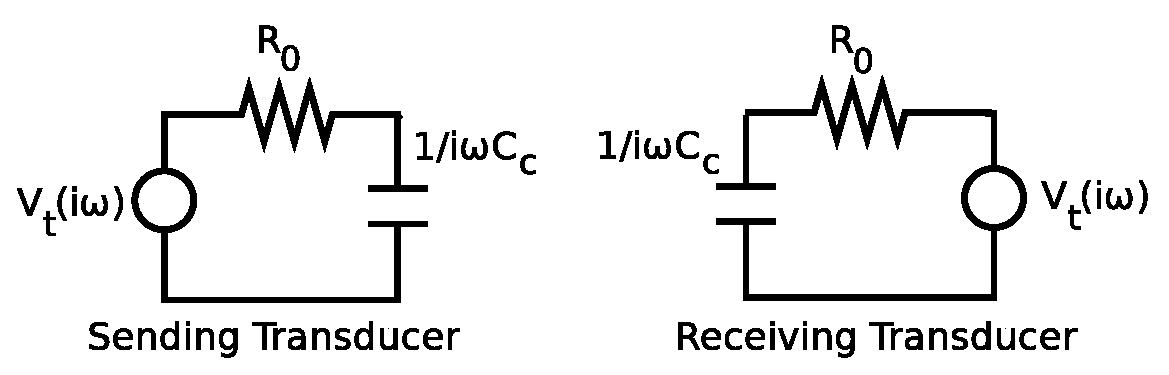
\includegraphics[width=12.70cm,height=5.60cm]{trans_circ.eps}
\end{center}
% \vspace*{-20 pt}
 \caption[des1]
%>>>> use \label inside caption to get Fig. number with \ref{}
   { \label{equiv_circ}
Equivalent circuit diagrams for the sending and receiving
transducers, showing the transducer voltages along with their
equivalent capacitance; $C_c = \overline{\varepsilon}_{33}\pi
a^2/l$.}
\end{figure}
The reflection and transmission coefficients ${\bf R}$ and ${\bf
T}$ at $x = l$ can be found as
\begin{equation}
{\bf R} = \frac{\overline{C_{33}}+
\frac{\overline{d_{33}}d_{33}}{2s^E_{33}} -
C^\ast_{33}}{\overline{C_{33}}+
\frac{\overline{d_{33}}d_{33}}{2s^E_{33}} + C^\ast_{33}}
\label{refcof1}
\end{equation}
\begin{equation}
{\bf T} = \frac{2\left(\overline{C_{33}}+
\frac{\overline{d_{33}}d_{33}}{2s^E_{33}}\right)}{\overline{C_{33}}+
\frac{\overline{d_{33}}d_{33}}{2s^E_{33}} + C^\ast_{33}}
\label{transcof1}
\end{equation}
The same relations hold for signals originating in transducer B
and propagating into the rod.  The reflection and transmission
coefficients $\hat{\bf R}$ and $\hat{\bf T}$ at $z=L+l$ can also
be found,
%
\begin{align}
&\hat{\bf R} = \frac{C^\ast_{33} - \overline{C}_{33} -
\frac{\overline{d_{33}}d_{33}}{s^E_{33}}}{C^\ast +
\overline{C}_{33} +
\frac{\overline{d_{33}}d_{33}}{s^E_{33}}} \nonumber\\
&\hat{\bf T} = \frac{2C^\ast_{33}}{\overline{C}_{33} +
\frac{\overline{d_{33}}d_{33}}{s^E_{33}}+ C^{\ast}_{33}}
\label{rbar2}
\end{align}

These relations also apply for signals traveling through the rod
to transducer A.  If the voltage across a chosen transducer is
measured by a high input-impedance voltage sensor, it provides the
signal to be reversed (and amplified). With the Fourier transform
of a signal $x(t)$ defined as $x(i\omega)$, the Fourier transform
of the time reversed version $x(-t)$ is $x^{\star}(i\omega)$,
where ${}^\star$ denotes complex conjugate.

In parts of the analysis to follow, we introduce a parameter $\nu$
to represent a spatial attenuation of $\exp(-\nu l_p)$ over a
propagation distance $l_p$ (see also section \ref{sect:vib}).

%\nomenclature{$w_{Rt}(t); {w}_{Rt}(i\omega)$}{Deflection due to
%time reversed and
%amplified voltage at the receiving transducer; its Fourier transform}%
%%\nomenclature{${\hat w}_{Rt}$}{Laplace transform of $w_{Rt}$}
%\nomenclature{$w_n; {w}_n(i\omega)$}{Deflection due to the second
%pulse generated by the sending transducer; its Fourier transform}

\subsection{Time Reversal in the Presence of a Defect}
\label{sect:timerevth}

Here we consider the effect of a single planar defect at an {\em a
priori} unknown coordinate along the length of the rod.  As long
as signal reversal is carried out correctly, it is not necessary
to know the defect location for the reversal and focusing to
occur.  In the sequence of events modeled, we have a
right-propagating original pulse generated by transducer A, which
encounters the defect and is split into a part that propagates
back to transducer A and a part that continues on further until it
reaches transducer B.  These can be quantified using complex
reflection and transmission coefficients at the defect. If the
defect is modeled as a local change in $C^\ast_{33}$ to
$C^c_{33}$, and $\rho^\ast$ to $\rho^c$, then the following
conditions can be applied at the defect.
\begin{equation}
1+\overline{\bf R} = \overline{\bf T} \label{defect1}
\end{equation}
and
\begin{equation}
T^+_3(l^-_c,t) = T^+_3(l^+_c,t) \label{defect2}
\end{equation}
%
From equations (\ref{defect1}) and (\ref{defect2}) and based on
previous treatment, we can infer $\overline{\bf R}$ and
$\overline{\bf T}$ as,
\begin{align}
&\overline{\bf R} = \frac{C^\ast_{33} - C^c_{33}}{C^\ast_{33} +
C^c_{33}} \nonumber\\
&\overline{\bf T} = \frac{2C^\ast_{33}}{C^\ast_{33}+C^c_{33}}
\label{reftransdef}
\end{align}%
%\nomenclature{$C^c_{33}$}{Local elastic constant modeling defect}%
\nomenclature{$\overline{\bf R}$}{Complex reflection coefficient
at defect}%
\nomenclature{$\overline{\bf T}$}{Complex transmission coefficient
at defect}%

As before, implementation of time reversed focusing does not
require {\em a priori} knowledge of $\overline{\bf R}$ and
$\overline{\bf T}$. The strain under the pulse returning to
transducer A from the defect can be expressed as,
\begin{equation}
\frac{\partial w_{cr}}{\partial z} = \overline{\bf R}\frac{\partial
w_t}{\partial z}; \ \left(\frac{l}{c} \leq t \leq
\frac{l}{c}+\frac{L}{c^\ast}\right) \label{defrefl1}
\end{equation}
where
\begin{equation}
\frac{\partial w}{\partial z} = {\bf T}\frac{\partial w}{\partial
z}\nonumber
\end{equation}
The part of the pulse proceeding to the receiving transducer B as,
\begin{equation}
\frac{\partial w_{ct}}{\partial z} = \overline{\bf T}\frac{\partial
w_t}{\partial z}; \ \left(\frac{l}{c} \leq t \leq
\frac{l}{c}+\frac{L}{c^\ast}\right) \label{deftrans1}
\end{equation}
\nomenclature{$l_c$}{Crack location, {\em a priori} unknown}%
The pulse $\frac{\partial w_{cr}}{\partial z}$ returns to the
sending transducer A at $t = \frac{l}{c}+\frac{2l_c}{c^\ast}$. The
voltage created at the sending transducer A, ignoring spatial
dissipation for now,
\begin{equation}
V^{+}_s(i\omega) = -\frac{d_{33}\pi
a^2}{2s^E_{33}C_c}\frac{\partial w_{cr}}{\partial z}(i\omega)
\label{vsenddefect}
\end{equation}
\nomenclature{$V^+_s(t), V^+_s(i\omega)$}{Voltage created at
transducer A by pulse returning from defect} where
\begin{equation}
\frac{\partial w_{cr}}{\partial z}(i\omega) = {\hat{\bf
T}}\overline{\bf R}{\bf T}\frac{{\partial w}}{\partial
z}(i\omega)\times{\exp
}\left[{-i\omega\left(\frac{l}{c}+\frac{2l_c}{c^\ast}\right)}\right]
\label{strnsenddefect}
\end{equation}
$V^{+}_s(t)$ is measured by a high input-impedance sensor,
amplified, and played back in reverse to create a new pulse, which
at the defect causes a strain.  This is,
%\begin{equation}
%\frac{\partial { w}_{sR}}{\partial z}(i\omega) = i{\bf
%T}M{\hat{\bf R}}\left(\frac{2s^E_{33}C_c}{d_{33}\pi
%a^2}\right)\left(\frac{\overline{\bf R}{\bf
%T}}{R_0C_c}\right)\left(\frac{1}{i\omega +
%\frac{1}{R_0C_c}}\right)\frac{\partial { w}}{\partial
%z}(i\omega)\times\exp\left[{i\omega\left(\frac{2l}{c^\ast}+\frac{2l}{c}\right)}\right];
%\ {\rm at}\ z = l_c \label{newpulsesend}
%\end{equation}
\nomenclature{$\frac{\partial w}{\partial z}(t)$; $\frac{\partial
w}{\partial z}(i\omega)$}{Strain created in the sending transducer
A; its Fourier transform}%
\nomenclature{$\frac{\partial
w_{sR}}{\partial z}(t)$; $\frac{\partial w_{sR}}{\partial
z}(i\omega)$}{Strain
under reversed pulse caused by sending transducer A; its Fourier transform}%
\nomenclature{$\frac{\partial w_{tR}}{\partial z}(t)$;
$\frac{\partial w_{cR}}{\partial z}(i\omega)$}{Strain
under focused pulse at `defect' transducer; its Fourier transform}%
\nomenclature{$\frac{\partial w_{cR}}{\partial z}(t)$;
$\frac{\partial w_{tR}}{\partial z}(i\omega)$}{Strain
under reversed pulse caused by receiving transducer B; its Fourier transform}%

\begin{equation}
\frac{\partial { w}_{sR}}{\partial z}(i\omega) =
i\left(\frac{\hat{\bf T}M{\bf T}^2\overline{\bf
R}}{R_0C_c}\right)\left(\frac{1}{i\omega +
\frac{1}{R_0C_c}}\right)\frac{\partial {w}}{\partial
z}(i\omega)\times \exp
\left[{i\omega\left(\frac{3l_c}{c^\ast}+\frac{2l}{c}\right)}\right]
\label{strdefect1}
\end{equation}
The transmitted part of the pulse reaches transducer B at a
distance $l_T$ away $(l_T + l_c = L)$.  The strain under it is
\begin{equation}
\frac{\partial { w}_{ct}}{\partial z} = \overline{\bf
T}\frac{\partial {w}_t}{\partial z}; \ z = L \label{strreceiv1}
\end{equation}
%
The voltage this creates across the receiving transducer is,
\begin{equation}
V^+_t(i\omega) =  i\frac{d_{33}\pi a^2}{2s^E_{33}C_c}\hat{\bf
T}\frac{\partial { w}_{ct}}{\partial z}(i\omega)
\label{voltreceiv2}
\end{equation}
%
Inserting equation (\ref{strreceiv1}) into equation
(\ref{voltreceiv2}),
\begin{equation}
V^+_t(i\omega) = i\frac{\overline{\bf T}\hat{\bf T}{\bf
T}d_{33}\pi a^2}{2s^E_{33}C_c}\frac{\partial {w}}{\partial
z}(i\omega)\times{\exp}\left[{-i\left(\frac{L}{c^\ast}+
\frac{l}{c}\right)}\right] \label{voltreceiv3}
\end{equation}
When this voltage (as measured by a high input-impedance sensor) is
reversed and played back with magnification, the strain under the
pulse is found to be,
\begin{equation}
\frac{\partial {w}_{tR}}{\partial z}(i\omega) =
-i\left(\frac{M{\bf T}^2\overline{\bf T}{{\bf
T}}}{R_0C_c}\right)\left(\frac{1}{i\omega +
\frac{1}{R_0C_c}}\right)\frac{\partial {w}}{\partial
z}(i\omega)\times{\exp}\left[{i\omega\left(\frac{L}{c^\ast}+
\frac{2l}{c}\right)}\right] \label{strplaybk1}
\end{equation}
At the defect, this strain becomes,
\begin{equation}
\frac{\partial { w}_{tR}}{\partial z}(i\omega) =
-i\left(\frac{M{\bf T}^2\overline{\bf T}{\hat {\bf
T}}}{R_0C_c}\right)\left(\frac{1}{i\omega +
\frac{1}{R_0C_c}}\right)\frac{\partial {w}}{\partial
z}(i\omega)\times{\exp}\left[{i\omega\left(\frac{L}{c^\ast}+
\frac{2l}{c}+ \frac{l_T}{c^\ast}\right)}\right]
\label{strplaybkdef1}
\end{equation}
%
We know that the time taken for the pulse reflected from the defect
to return to the sending transducer is easily measured.  Denoting
this as $\Delta_c$, we have
\begin{equation}
2l_c = \Delta_c c^\ast \label{speed1}
\end{equation}
Similarly, the time taken for the signal transmitted through the
defect reaches the receiving transducer at a time $\Delta_t$ such
that
\begin{equation}
L = \Delta_t c^\ast \label{speed2}
\end{equation}
The reversal must begin only after a time $\Delta_M$ such that
\begin{equation}
\Delta_M = \max(\Delta_c, \Delta_t) \label{DeltaM}
\end{equation}
\nomenclature{$\Delta_c, \Delta_t; \Delta_M, \Delta_m$}{Time taken
for pulse to return to transducer A from defect, reach transducer
B, the
greater, the smaller of the two}%
One of the transducers must therefore play back a minimum idle
period.
\begin{equation}
\Delta_i = \Delta_M - \Delta_m \label{Deltai}
\end{equation}
where
\begin{equation}
\Delta_m = \min(\Delta_c, \Delta_t) \label{Deltam}
\end{equation}
If $\Delta_m = \Delta_t$, corresponding to $l_c > l_T$, then the
played-back pulse from the receiving transducer should arrive back
at the defect at
\begin{equation}
t^t_{def} = \frac{L}{c^\ast}+\frac{2l}{c} + \frac{l_T}{c^\ast} +
\Delta_i \label{thatt}
\end{equation}
The pulse played back by the sending transducer should arrive at
\begin{equation}
t^s_{def} = \frac{3l_c}{c^\ast} + \frac{2l}{c} \label{thats}
\end{equation}
It is easily seen, since $\Delta_i = \Delta_s - \Delta_t$, that
$t^t_{def}$ as given by equation (\ref{thatt}) equals
\begin{equation}
t^t_{def} = \frac{3l_c}{c^\ast} + \frac{2l}{c} = t^s_{def}
\label{tequal}
\end{equation}
as desired.  The reversed and amplified pulses from both
transducers are found to arrive at the defect at the same instant.
They are both diffused by a small amount corresponding to the
factor ${(i\omega + 1/R_0C_c)}^{-1}$ in equations
(\ref{strdefect1}) and (\ref{strplaybkdef1}).  When the defect is
closer to the receiving transducer, i.e, $l_c > l_T$, the strain
distribution under the pulse is,
\begin{align}
\frac{\partial { w}_{sR}}{\partial z}(l_c,i\omega) +
\frac{\partial { w}_{tR}}{\partial z}(l_c,i\omega) =
&-i\left(\frac{{\hat \bf T}M{\bf T}^2\overline{\bf
R}}{R_0C_c}\right)\left(\frac{1}{i\omega +
\frac{1}{R_0C_c}}\right)\frac{\partial { w}}{\partial
z}(i\omega)\times{\exp}\left[{i\omega\left(\frac{3l_c}{c^\ast}+\frac{2l}{c}\right)}\right]\nonumber\\
- &i\left(\frac{M{\bf T}^2\overline{\bf T}{\hat{\bf
T}}}{R_0C_c}\right)\left(\frac{1}{i\omega +
\frac{1}{R_0C_c}}\right)\frac{\partial {w}}{\partial
z}(i\omega)\times{\exp}\left[{i\omega\left(\frac{L}{c^\ast}+
\frac{2l}{c}+ \frac{l_T}{c^\ast} + \Delta_i\right)}\right]
\label{combstrdef1}
\end{align}
When the defect is closer to the sending transducer,
\begin{align}
\frac{\partial { w}_{sR}}{\partial z}(l_c,i\omega) +
\frac{\partial { w}_{tR}}{\partial z}(l_c,i\omega) =
&-i\left(\frac{{\bf T}^2M{\bf T}^2\overline{\bf
R}}{R_0C_c}\right)\frac{\partial {w}}{\partial
z}(i\omega)\left(\frac{1}{i\omega +
\frac{1}{R_0C_c}}\right)\times{\exp}\left[{i\omega\left(\frac{3l_c}{c^\ast}+\frac{2l}{c}+
\Delta_i\right)}\right]\nonumber\\
+-i&\left(\frac{M{\bf T}^2\overline{\bf T}{\hat{\bf
T}}}{R_0C_c}\right)\left(\frac{1}{i\omega +
\frac{1}{R_0C_c}}\right)\frac{\partial {w}}{\partial
z}(i\omega)\times{\exp}\left[{i\omega\left(\frac{L}{c^\ast}+
\frac{2l}{c}+ \frac{l_T}{c^\ast} + \Delta_i\right)}\right]
\label{combstrdef2}
\end{align}
The combined strain at the defect in the two cases may be written
as,
\begin{align}
\frac{\partial {w}_c}{\partial z}(i\omega) =
&-i\left(\frac{{\hat{\bf T}}M{\bf
T}^2}{R_0C_c}\right)\left(\overline{\bf R}+\overline{\bf
T}\right)\left(\frac{1}{i\omega+\frac{1}{R_0C_c}}\right)\frac{\partial
{w}}{\partial z}(i\omega)
\nonumber\\
&\times\exp\left[i\omega\left(\frac{3l_c}{c^\ast}+\frac{2l}{c}\right)\right];\
\ \Delta_c > \Delta_t \label{strtotaldef1}
\end{align}
and,
\begin{align}
\frac{\partial { w}_c}{\partial z}(i\omega) =
&\left(\frac{{\hat{\bf T}}M{\bf
T}^2}{R_0C_c}\right)\left(\overline{\bf R}+\overline{\bf
T}\right)\left(\frac{1}{i\omega+\frac{1}{R_0C_c}}\right)\frac{\partial
{ w}}{\partial z}(i\omega)
\nonumber\\
&\times\exp\left[-i\omega\left(\frac{3l_c}{c^\ast}+\frac{2l}{c}\right)\right];\
\ \Delta_t > \Delta_c \label{strtotaldef2}
\end{align}
%Finally,  inverse Fourier transformation of equation
%(\ref{rightfocus1}) leads to the time-domain variation for the
%pulse height when focused at the sending transducer A. Performing
%this step and modeling the spatial attenuation rate as $\nu$,
%\begin{align}
%\frac{\partial w_c}{\partial z}(l,t) = &-\frac{2s^E_{33}{\bf
%T}V_0\delta(t)}{d_{33}\pi a^2R_0}\left(1+\frac{{\bf T}{\hat {\bf
%T}}M}{R_0C_c}\exp\left(-2\nu (L-l)\right)\right)\times \nonumber\\
%&{\exp\left[-\frac{t}{R_0C_c}\right]}; \ \ t \geq
%\frac{2L}{c^\ast}+\frac{2l}{c} \label{sendingtime1}
%\end{align}
%On the other hand,
The focused pulse at the defect thus has the following time domain
form,
\begin{align}
&\frac{\partial w_c}{\partial z}(l_c,t) = -\frac{2s^E_{33}{\bf
T}}{d_{33}\pi a^2R_0}V_0\delta(t)\left(\frac{{\hat{\bf T}}M{\bf
T}}{R_0C_c}\right)\left(\overline{\bf R}\exp\left(-2\nu
l_c\right)+\overline{\bf
T}\exp\left(-2\nu l_T\right)\right)\times \nonumber\\
&{\exp}\left[{-\frac{1}{R_0C_c}\left(t-\frac{3l_c}{c^\ast}-\frac{2l}{c}\right)}\right];
\ \ t \geq \frac{3l_c}{c^\ast}+\frac{2l}{c} \label{defecttime1}
\end{align}

where we have also included the effect of the spatial dissipation
rate $\nu$.  Since the voltage applied to the actuator above is an
impulse approximately modeled as the Dirac Delta function, the
function representing the strain in equation (\ref{defecttime1})
can be considered unit impulse response functions with $V_0 = 1$
for strain under the corresponding focused signal. Alternatively,
they are the Green's functions for the strain at the point of
focusing. Thus, defining
%\begin{align}
%h_{act}(t) \equiv G_{act}(l,l; 0,t) = &-\frac{2s^E_{33}{\bf
%T}}{d_{33}\pi a^2R_0}\left(1+\frac{{\bf T}{\hat {\bf
%T}}M}{R_0C_c}\exp(-2\nu L)\right)\times \nonumber\\
%&\delta(t)\exp{\left[-\frac{1}{R_0C_c}\left(t-\frac{2L}{c^\ast}-\frac{2l}{c}\right)\right]};
%\ \ t \geq \frac{2L}{c^\ast}+\frac{2l}{c} \label{imptrans}
%\end{align}
%\nomenclature{$h_{act}(t)$}{Impulse response function for the
%focused pulse at the sending transducer}
%\nomenclature{$G_{act}(x,\xi;0,t)$}{Green's function showing the
%influence at $x$ of the time reversed focused pulse at $\xi$}
%Similarly,
\begin{align}
&h_{def}(t) \equiv G_{def}(l,l_c; 0,t) = -\frac{2s^E_{33}{\bf
T}}{d_{33}\pi a^2R_0}\left(\frac{{\hat{\bf T}}M{\bf
T}}{R_0C_c}\right)\left(\overline{\bf R}\exp(-2\nu
l_c)+\overline{\bf
T}\exp(-2\nu l_T)\right)\times \nonumber\\
&\delta(t)\exp{\left[-\frac{1}{R_0C_c}\left(t-\frac{3l_c}{c^\ast}-\frac{2l}{c}\right)\right]};
\ \ t \geq \frac{3l_c}{c^\ast}+\frac{2l}{c} \label{impdefect}
\end{align}%

\nomenclature{$h_{def}(t)$}{Impulse response function for the
focused pulse at the defect}
\nomenclature{$G_{def}(x,\xi;0,t)$}{Green's function showing the
influence at $x$ of the time reversed focused pulse at $\xi$}

Consistent with the present small-signal linear theory based
treatment, the strain under  a focused waveform created by an
arbitrary voltage input at the sending transducer  A can be
calculated using the Green's functions above.  Here we use %a
%triangular voltage pulse [(found to be optimal for crack healing
%because it yields a constant strain across the defect (Korde et
%al, ICHM, 2009)], and
a multi-tone chirp signal. Representing the prescribed input
signal as $V(t)$ (see section \ref{sect:vib}), the strain
variations under the focused signal at the defect can be found
using,
%\begin{equation}
%S_{act}(t) = \int_0^t h_{act}(\tau)V(t-\tau)d\tau \label{strconv1}
%\end{equation}
\begin{equation}
S_{def}(t) = \int_0^t h_{def}(\tau)V(t-\tau)d\tau \label{strconv2}
\end{equation}
We define $P$, the voltage required to produce unit strain as
\begin{equation}
P = \frac{d_{33}\pi a^2 R_0}{2 s^E_{33}} \label{gam1}
\end{equation}%
 This is required because $h_{def}$ relates voltage to strain.
 Realizing that $S_{def}$ above are the strains
 resulting from the first time reversal \cite{fink}, the results of the next
 iteration in the two cases can be written as
 %\begin{equation}
% S^{(2)}_{act}(t) =
% P\int_0^th_{act}(\tau)S_{act}(t-\tau)d\tau
% \label{secondact}
% \end{equation}
% and
\begin{equation}
 S^{(2)}_{def}(t) =
 P\int_0^th_{def}(\tau)S_{def}(t-\tau)d\tau
 \label{seconddef}
 \end{equation}
 Following Ref. \cite{fink} we can reexpress equation
 (\ref{seconddef}) in frequency domain by
 applying the Fourier transform to write,
\begin{equation}
S^{(2)}_{def}(i\omega) = P H_{def}(i\omega)S^{(1)}_{def}(i\omega)
\label{spec2}
\end{equation}
%\nomenclature{$S^{(n)}_{act}(t)$, $S^{(n)}_{act}(i\omega)$}{Strain
%at
%the actuator after the nth iteration; its Fourier transform}%
\nomenclature{$S^{(n)}_{def}(t)$, $S^{(n)}_{def}(i\omega)$}{Strain
at the
defect after the nth iteration; its Fourier transform}%
%\nomenclature{$H_{act}(i\omega)$}{Fourier transform of Green's
%function; i.e. frequency response function at actuator}%
\nomenclature{$H_{def}(i\omega)$}{Fourier transform of Green's
function; i.e. frequency response function at defect}%
The Fourier-transformed time reversed strain resulting from
equation (\ref{spec2}) is $S^{\star (2)}_{def}$.  Therefore a
third focusing at the defect leads to
\begin{equation}
%&S^{\star (3)}_{act}(i\omega) =
%P^2H_{act}(i\omega)H^{\star}_{act}(i\omega)S^{(1)}_{act}(i\omega)\nonumber\\
%&
S^{\star (3)}_{def}(i\omega) =
P^2H_{def}(i\omega)H^{\star}_{def}(i\omega)S^{(1)}_{def}(i\omega)
\label{spec3}
\end{equation}
In this way, the nth iteration ($n = 2m+1$) will cause,
\begin{equation}
%&S^{\star (n)}_{act}(i\omega) =
%P^{n-1}\left(H_{act}(i\omega)H^{\star}_{act}(i\omega)\right)^mS^{(1)}_{act}(i\omega)\nonumber\\
%&
S^{\star (n)}_{def}(i\omega) =
P^{n-1}\left(H_{def}(i\omega)H^{\star}_{def}(i\omega)\right)^mS^{(1)}_{def}(i\omega)
\label{specn}
\end{equation}

Each impulse response function includes a magnification factor
$M$. Thus, if $P \sim {\cal O}(10^{-1})$ then, choosing $M > {\cal
O}(10^{1})$ will allow that $P^{n-1} M^{n-1} = \chi^{n-1} > 1$,
where $\chi = PM$.  This will allow iterative growth in the
focused pulse amplitude until material dissipation helps bring
about convergence.

\section{EFFECT OF AXIAL VIBRATIONS}
\label{sect:vib}

Due to  the finite length of the rod, an impulsive excitation of
deflection or slope at one end can (in theory) generate all of the
rod's natural frequencies in axial vibration. Although dissipative
effects within the rod are expected to limit the build-up of
eigenfrequency vibrations, each time a pulse is applied and/or
played  back with amplification, new eigenfrequency vibrations are
generated.  We consider here conditions under which the local
strain caused by the successive reversed, amplified, and focused
signals above will exceed the accompanying eigenfrequency
vibration build up.

The vibration response of the rod to excitation of transducer A
can be modeled using the relation,
\begin{equation}
\rho^\ast \frac{\partial^2 {\tilde w}}{\partial t^2} - C^\ast_{33}
\frac{\partial^2 {\tilde w}}{\partial z^2} = 0 \label{vibax1}
\end{equation}%
\nomenclature{$\rho$}{Mass density of the rod material}%
%\nomenclature{$f(z,t)$}{Vibration causing applied force on rod}%
\nomenclature{$w_s(t)$}{Transducer caused deflection at $z=0$}%
with non-homogeneous boundary conditions ${\tilde w}(0,t) =
w_s(t)$, and ${\tilde w}(L,t) = 0$, where $w_s(t)$ is the
deflection produced by transducer A.  With a coordinate
transformation
\begin{equation}
{ w}(z,t) = {\tilde w}(z,t) + \frac{z-L}{L}{\ddot w}_s(t)
\label{wtilde}
\end{equation}
%\nomenclature{${\tilde w}(z,t)$}{Axial deformation of rod w}%
we have
\begin{equation}
\rho^\ast \frac{\partial^2 w}{\partial t^2} -
C^\ast_{33}\frac{\partial^2 w}{\partial z^2} = -\rho^\ast {\ddot
w}_s(t)\frac{z-L}{L} \label{wtransf}
\end{equation}
The eigenfunctions for the unforced problem corresponding to
equation (\ref{wtransf}) are
\[\phi_n(x) = \sin \beta_n z;\ \ \beta_n = \frac{n\pi}{L}\]
We may expand the solution $w(z,t)$ to equation (\ref{wtransf}) in
terms of these eigenfunctions as
\begin{equation}
w(z,t) = \sum_{m=1}^{\infty}\eta_m(t)\sin \beta_n z
\label{wvibexp}
\end{equation}

To account approximately for material damping, we use a
`mode-averaged' damping constant $c_d$, where $c_d$ is related to
$\nu$ according to,
\begin{equation}
\nu = \frac{c_d}{2\beta_n\sqrt{\rho^\ast C^{\ast}_{33}}}
\label{gameq1}
\end{equation}

Inserting equation (\ref{wvibexp}) into equation (\ref{wtransf}),
multiplying both sides by the eigenfunction $\phi_n(x)$ and
integrating from $0$ to $L$,
\begin{align}
&\rho{\ddot \eta}_n +c_d {\dot \eta}_n + C^\ast_{33}\beta^2_n \eta_n
= \nonumber\\
&-\frac{2\rho W_0}{L}{\ddot w}_s\left(
\frac{1-(-1)^n}{\beta^n}\right) \label{modaleq3}
\end{align}
%
%
Taking the Fourier transform of both sides and rearranging terms,
we have
%
\begin{equation}
\eta_n(i\omega) = -\frac{2\rho}{L}\left(
\frac{1-(-1)^n}{\beta^n}\right)\left(\frac{\omega^2w_s(i\omega)}{-\omega^2\rho
+ i c_d + C^\ast_{33}\beta^2_n}\right) \label{etan_fourier}
\end{equation}
%
which leads to,
\begin{equation}
\eta_n(t) = -\frac{2\rho}{2\pi L}\left(
\frac{1-(-1)^n}{\beta^n}\right)\int_{-\infty}^{\infty}\left(\frac{\omega^2w_s(i\omega)}{-\omega^2\rho
+ i c_d + C^\ast_{33}\beta^2_n}\right){\rm e}^{i\omega t}d\omega
\label{etan_t}
\end{equation}
%
For a finite (lasting $2 T$ seconds) multi-tone signal with a
bandwidth $\Delta \Omega$ \footnote{uniform amplitude distribution
is assumed.}), we may use
\begin{align}
w_s(t) = & \frac{2}{\pi (t-T)}\left(\cos \Omega t \sin \nabla
\Omega
t\right)\left(H(t-T) - H(t-2T)\right)\nonumber\\
& + \frac{2}{\pi (T-t)}\left(1-\cos \Omega t \sin \Delta \Omega
t\right)\left(H(t) - H(t-T)\right) \label{chirp}
\end{align}
%
$w(z,t)$ can be found by inserting $\eta_n(t)$ from equation
(\ref{etan_t}) into equation (\ref{wvibexp}).  Given that $w_s(t)$
decays as $\sim (1/t)$, with the addition of two zeros and two
complex poles, $w(z,t)$ will  be an oscillatory function over the
frequency range $[\Omega-\Delta \Omega, \Omega + \Delta \Omega]$
decaying at a rate $\sim (1/t^3)$.  Thus, the longer the delay
between successive time reversal iterations, the smaller will be
the vibration response within the rod.  Although the signal
amplitude increases by a factor $M$ at each iteration, a long
enough delay can be introduced to allow over an order of magnitude
decay in the vibration response.  In this case, as seen from
equation (\ref{specn}), while the focused pulse grows with
iteration number $n > 1$ as $M^{n-1}$, the vibration response will
grow as $M$.

\section{CALCULATIONS}
\label{sect:calc}

Calculations were carried out to help to visualize the
results obtained above and to provide a comparison for the
experimental results described in the following sections. For the
time reversal mirror calculations, combinations of two rods of circular
cross section were used (Figure \ref{tr_setup_1}). Three steel rods of different lengths were used for a total of three combinations. Their lengths
were $579$ mm, $437$ mm, and $428$ mm, with a diameter $12.7$ mm,
and a density $8.5 \times 10^3$ kg/m$^3$. Likewise, three nylon rods were used with their lengths being $148$ mm, $105$ mm, and $75$ mm with a diameter $12.7$ mm and a density $1.1 \times 10^3$ kg/m$^3$. The actuators were
piezoceramic stack actuators of diameter $13$ mm, clamped at the
two ends, with a piezoelectric strain constant of $d_{33} = 152
\times 10^{-12}$ C/N, and relative permittivity $\varepsilon_{33}
= 450 \varepsilon_0$, where $\varepsilon_0 = 8.854 \times
10^{-12}$ F/m. The elastic constant $C_{33}$ was taken to be $113
\times 10^9$ N/m$^2$, with the corresponding value for the steel
rods being $ C^\ast_{33} = 180 \times 10^9$ N/m$^2$ and for the nylon rods we have $ C^\ast_{33} = 2.1 \times 10^9$ N/m$^2$.  The
resistors $R_L = R_0 = 100 \Omega$.

\section{EXPERIMENTAL WORK}
\label{sect:expt}

%%Described below are tests performed to observe the evolution of
%%eigenfrequency vibrations, as well as the tests examining the time
%%reversed acoustics in the two cases: (i) focusing at the sending
%%transducer, and (ii) focusing at the defect.  Some of this work
%%was also presented in ref. \cite{AIAASelfHeal2010}.

Experiments were carried out to investigate iterative focusing at an arbitrary, a priori unknown defect location in one-dimension. The following section details the setup procedure, the hardware involved, and the signal processing algorithms that were used in performing the time reversal.

\subsection{Experimental Setup}
\label{sect:expSetup}

The setup included the use of two solid steel or nylon rod segments as the transmission medium. Three ceramic piezoelectric
transducers (PZTs) were used; two of them acted as both senders and
receivers while the third played the role of the `defect' and acted
only as a receiver. A thin layer of accelerometer putty was applied on the ends of the PZTs and the rods. The `defect' PZT was sandwiched between ends of
the two rods. The two send/receive PZTs (A and B) were each affixed to the remaining end of the rods. The setup is shown schematically below in
Figure \ref{tr_setup_1}. This system was then
placed in compression. The compression mechanism was made using optics table hardware, commonly available nuts and bolts, and some custom machined aluminum blocks. A single bolt was used to adjust the compression (Figure \ref{compression}). In the experiments, a small screw driver was used to turn the bolt one-quarter turn past finger tight. The experiments were performed on an optics table. Photographs of the apparatus as used in
the steel rod tests are shown in Figure \ref{tr_setup_2}. Figure \ref{tr_setup_3} shows the nylon rods ready for testing. 

\begin{figure}
\begin{center}
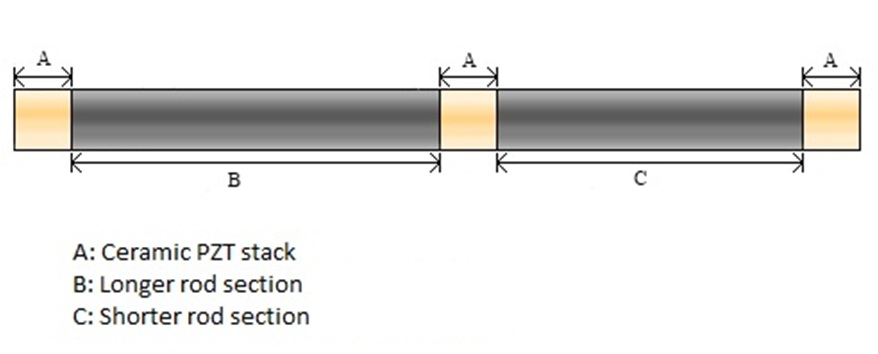
\includegraphics[width=13cm,height=5.8cm]{tr_dimensions}
\end{center}
% \vspace*{-20 pt}
 \caption[des1]
%>>>> use \label inside caption to get Fig. number with \ref{}
   { \label{tr_setup_1}
A schematic view of the test apparatus used. The PZTs had a length of 12mm. The PZT seen in the middle was the defect PZT. The PZTs on the ends were PZT A and PZT B. The two rods used in the setup were of different lengths and in the schematic this is simply noted as ``longer" and ``shorter" rod section. For the steel rods, the 3 length choices were $579$ mm, $437$ mm, and $428$ mm, which gave a total of 3 possible combinations ($579$ mm and $437$ mm, $579$ mm and $428$ mm, $437$ mm and $428$ mm). For the nylon rods, the 3 length choices were $148$ mm, $105$ mm, and $75$ mm, which also gave 3 possible combinations. The length choices for both the nylon and steel rods were arbitrary and unknown to the time reversal software }
\end{figure}

\begin{figure}
\begin{subfigmatrix}{2}
\subfigure[Left side compression mechanism]
{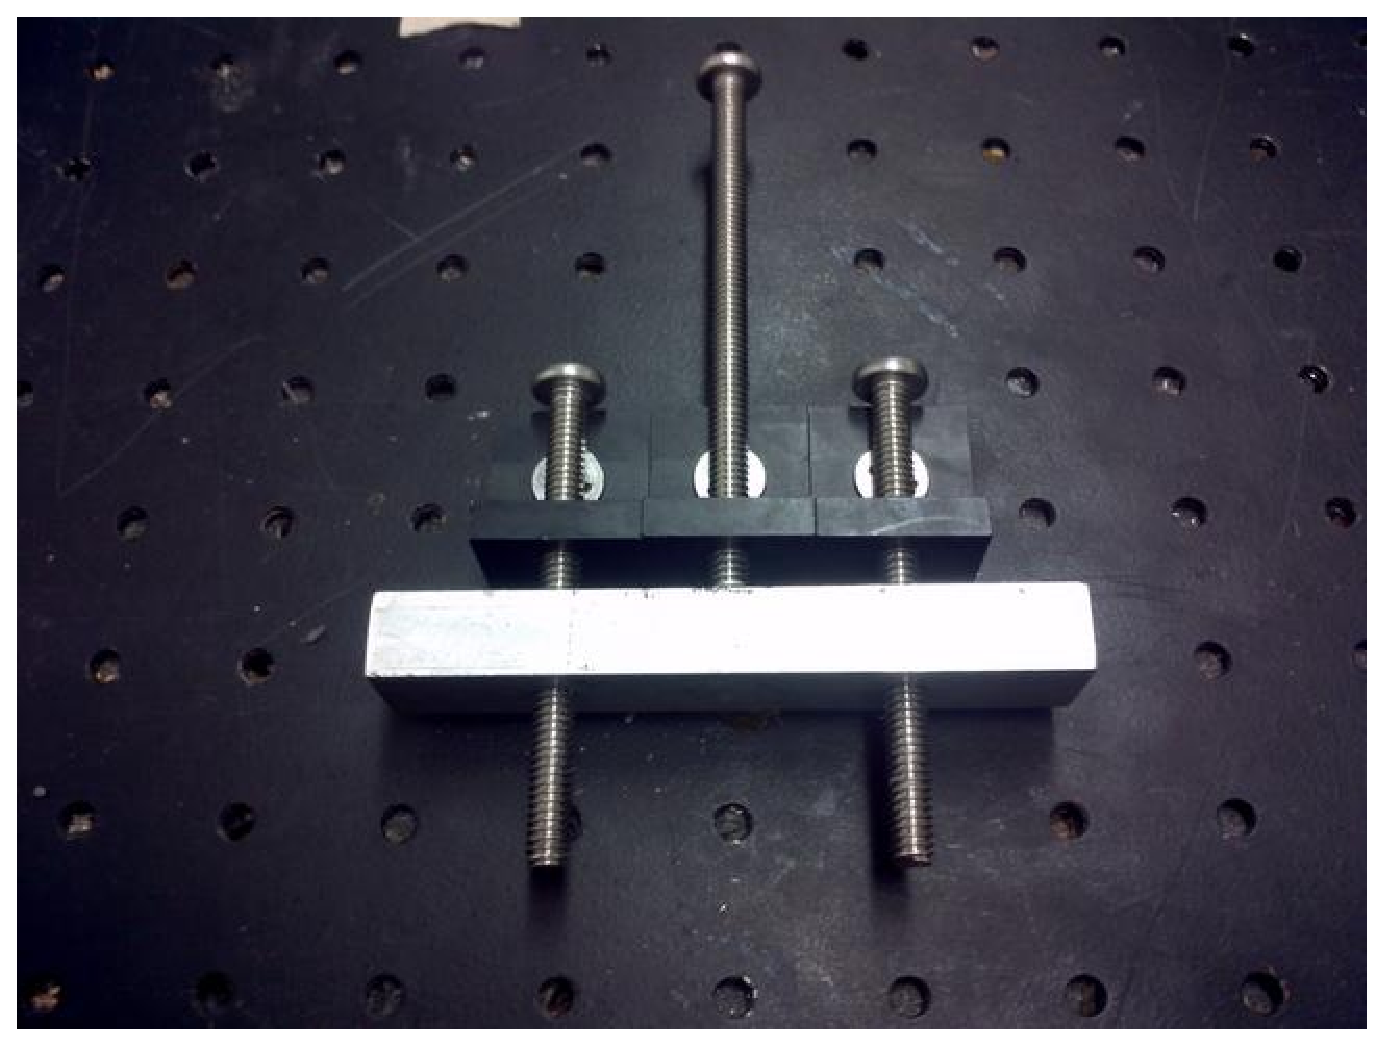
\includegraphics[width=9.7cm,height=5.75cm]{lsCompression.eps}}
\subfigure[Right side compression mechanism ]
{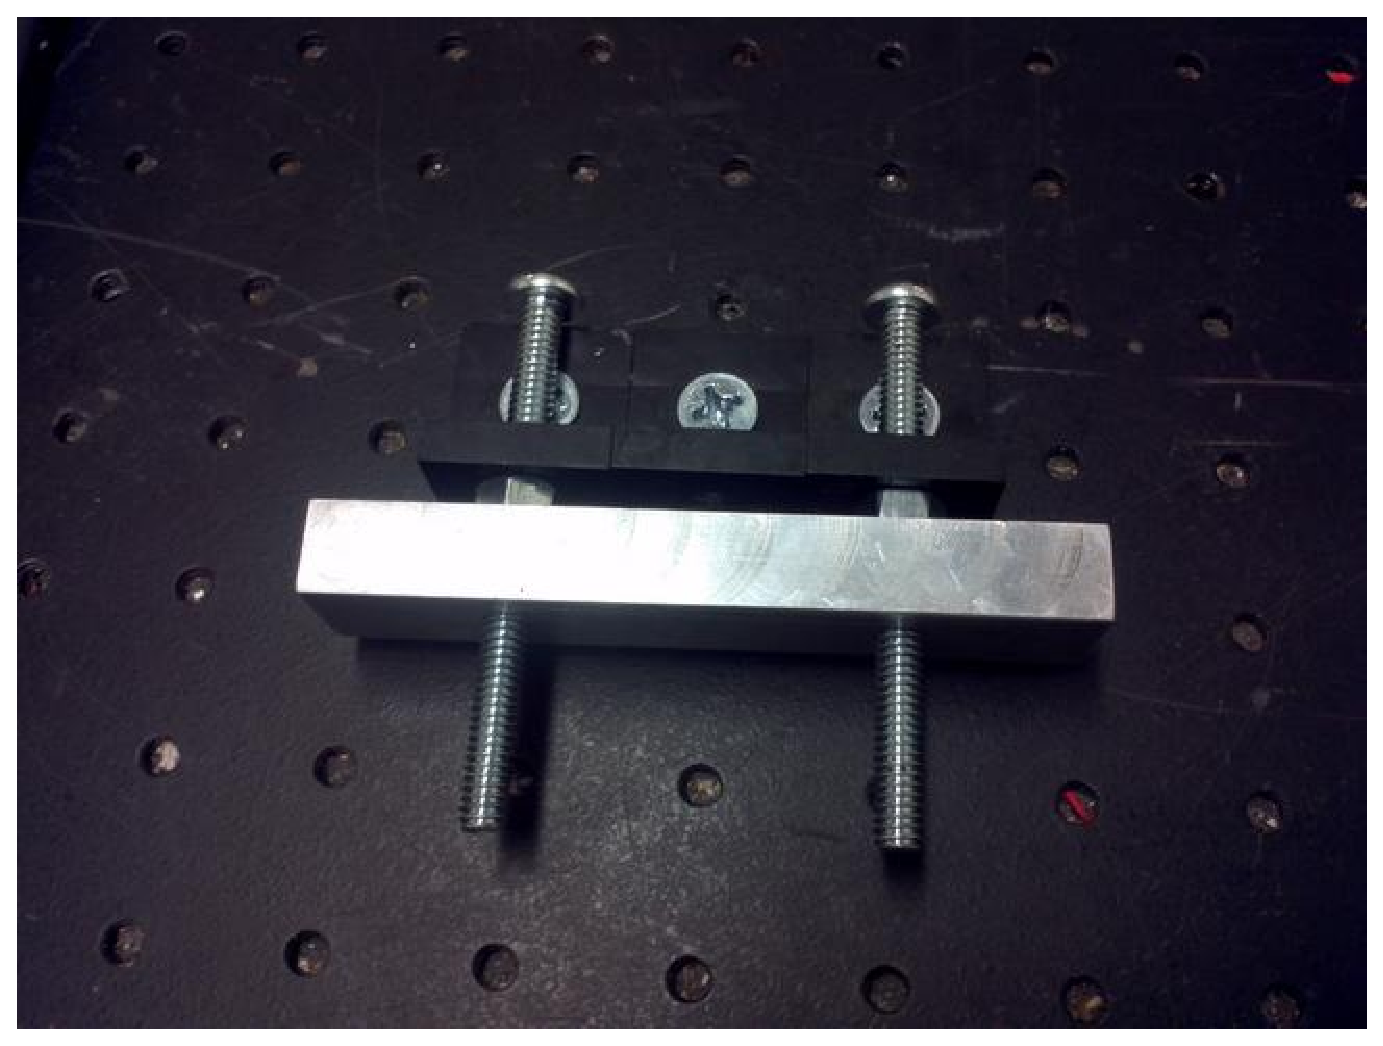
\includegraphics[width=9.7cm,height=5.75cm]{rsCompression.eps}}
\end{subfigmatrix}

   \caption[all]
%>>>> use \label inside caption to get Fig. number with \ref{}
   { \label{compression}
(a) The left side compression mechanism. The middle bolt was used to adjust the compression in the system by using it to move the aluminum block back and forth;
(b) Right side compression mechanism. This had two nuts to adjust the aluminum bar's positions so it could accommodate different rod sizes.
 }
   \end{figure}

%
\begin{figure}
\begin{subfigmatrix}{2}
\subfigure[Overview of Steel Rod Apparatus]
{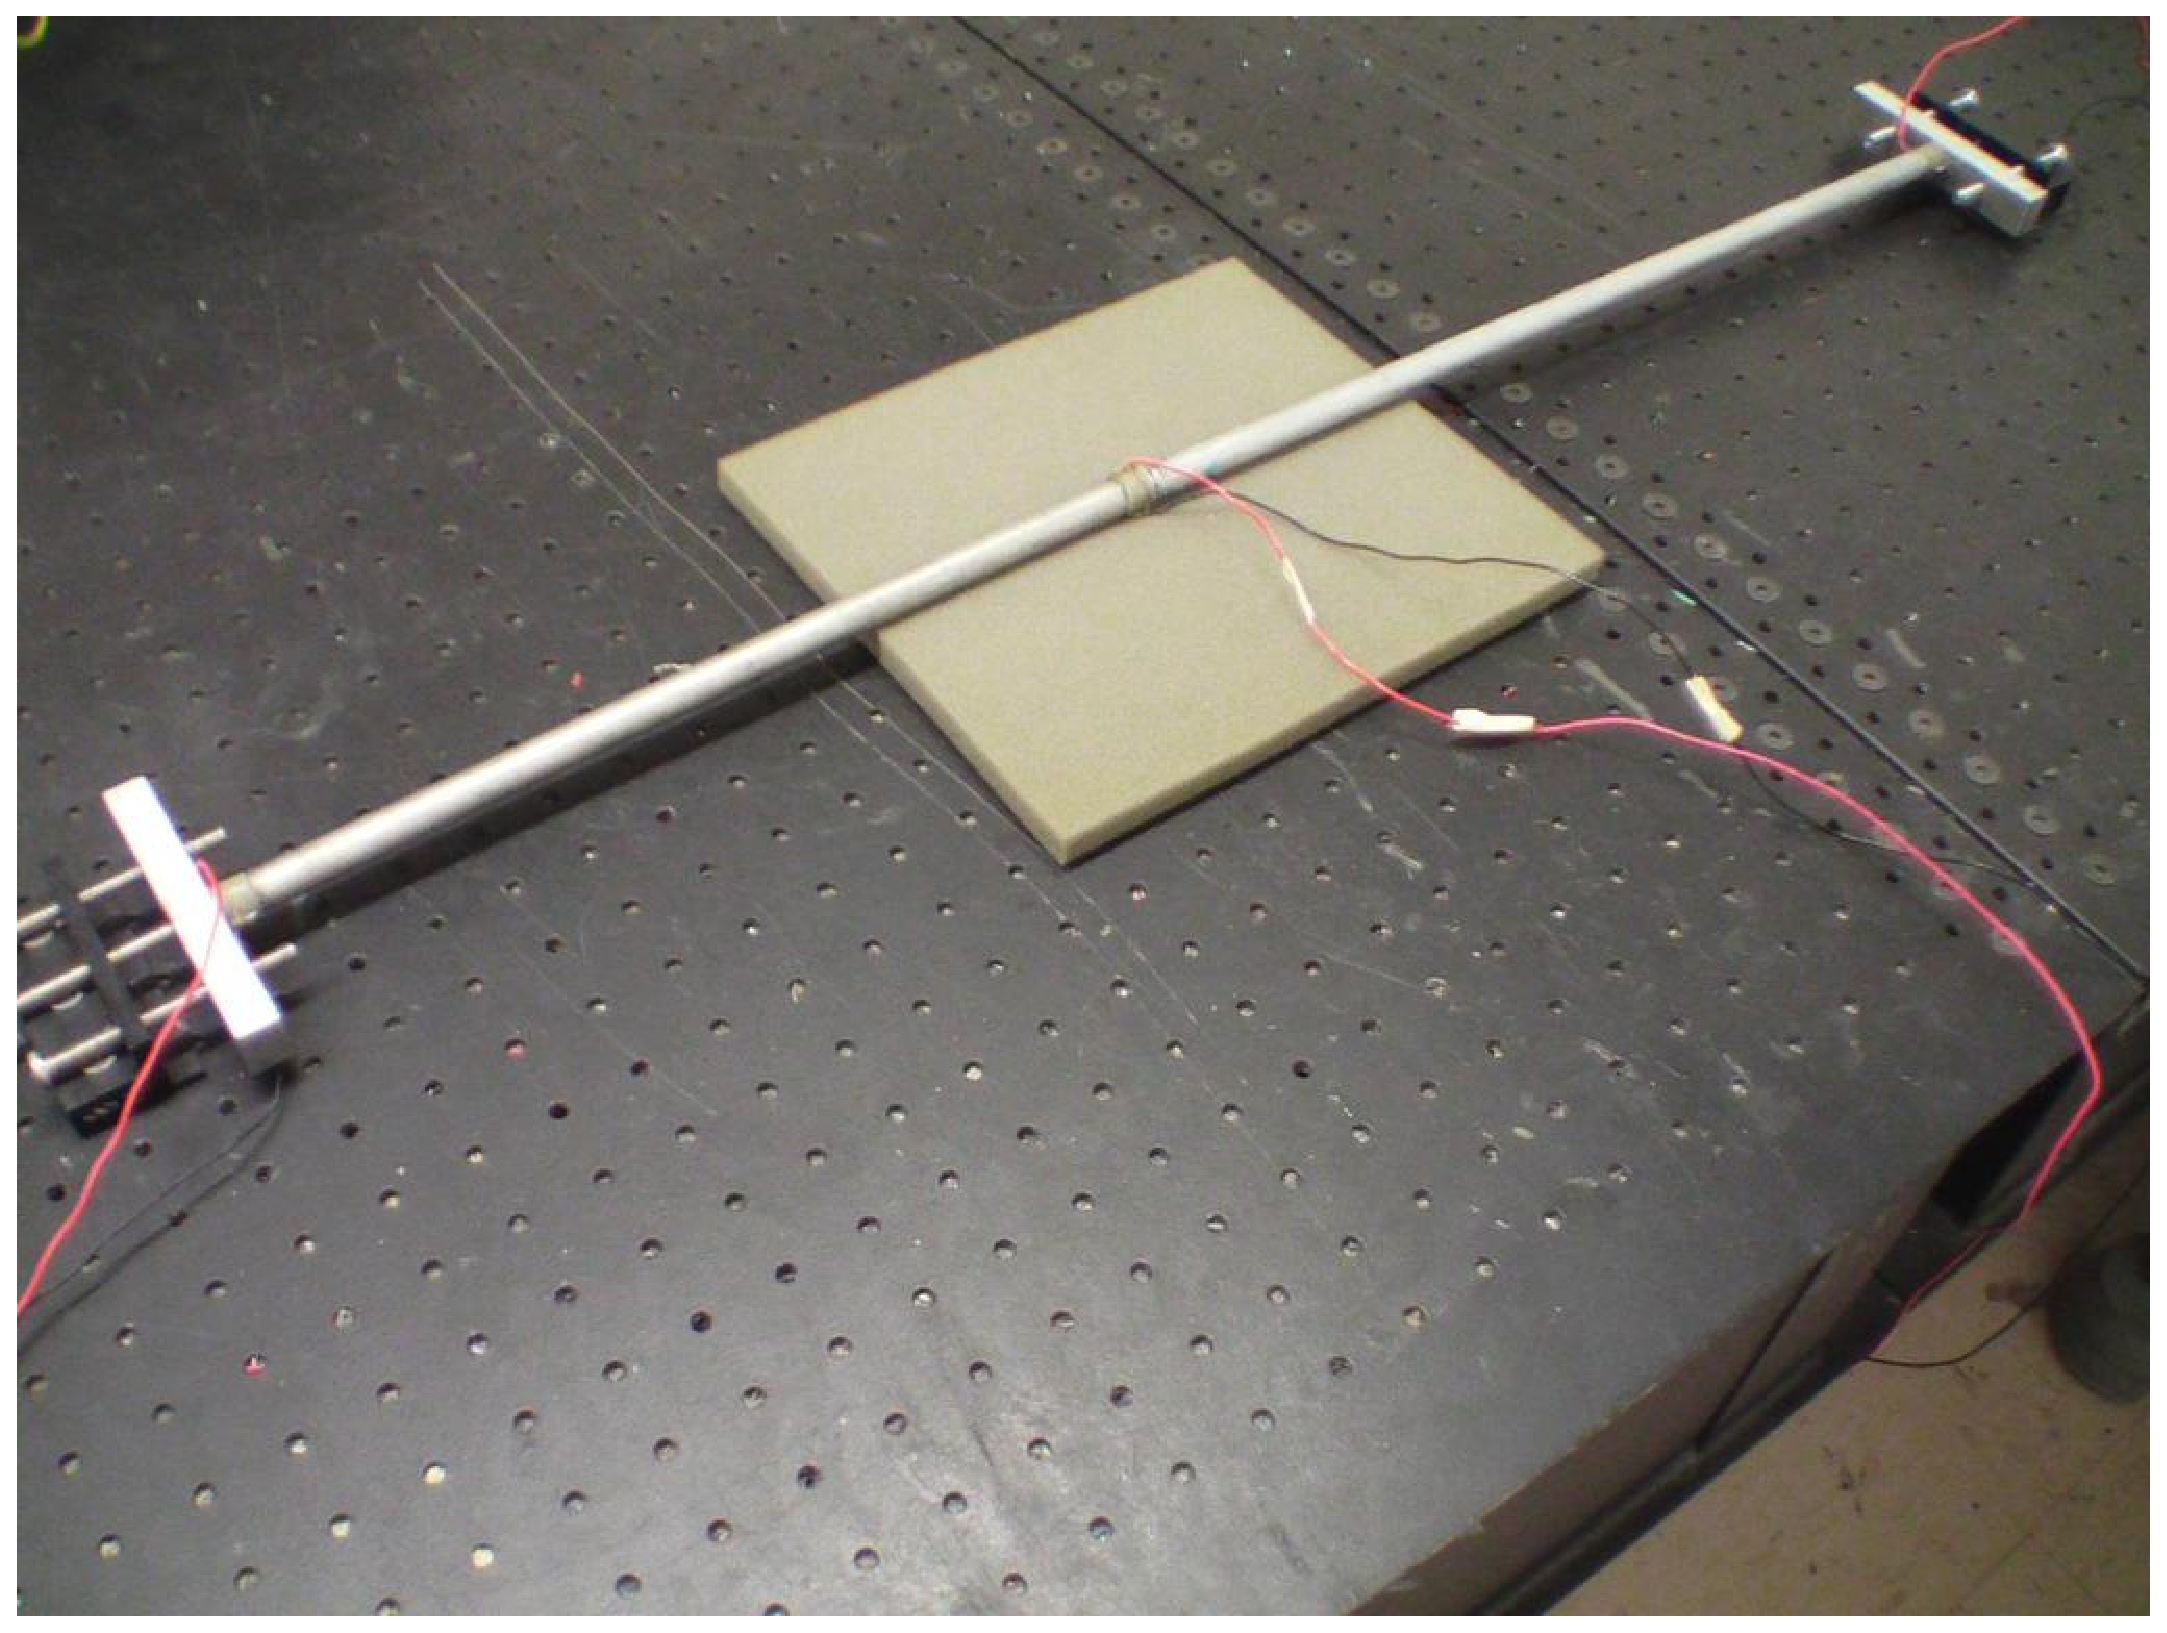
\includegraphics[width=9.7cm,height=5.75cm]{self_healing_setup1.eps}}
\subfigure[Closer View of Apparatus]
{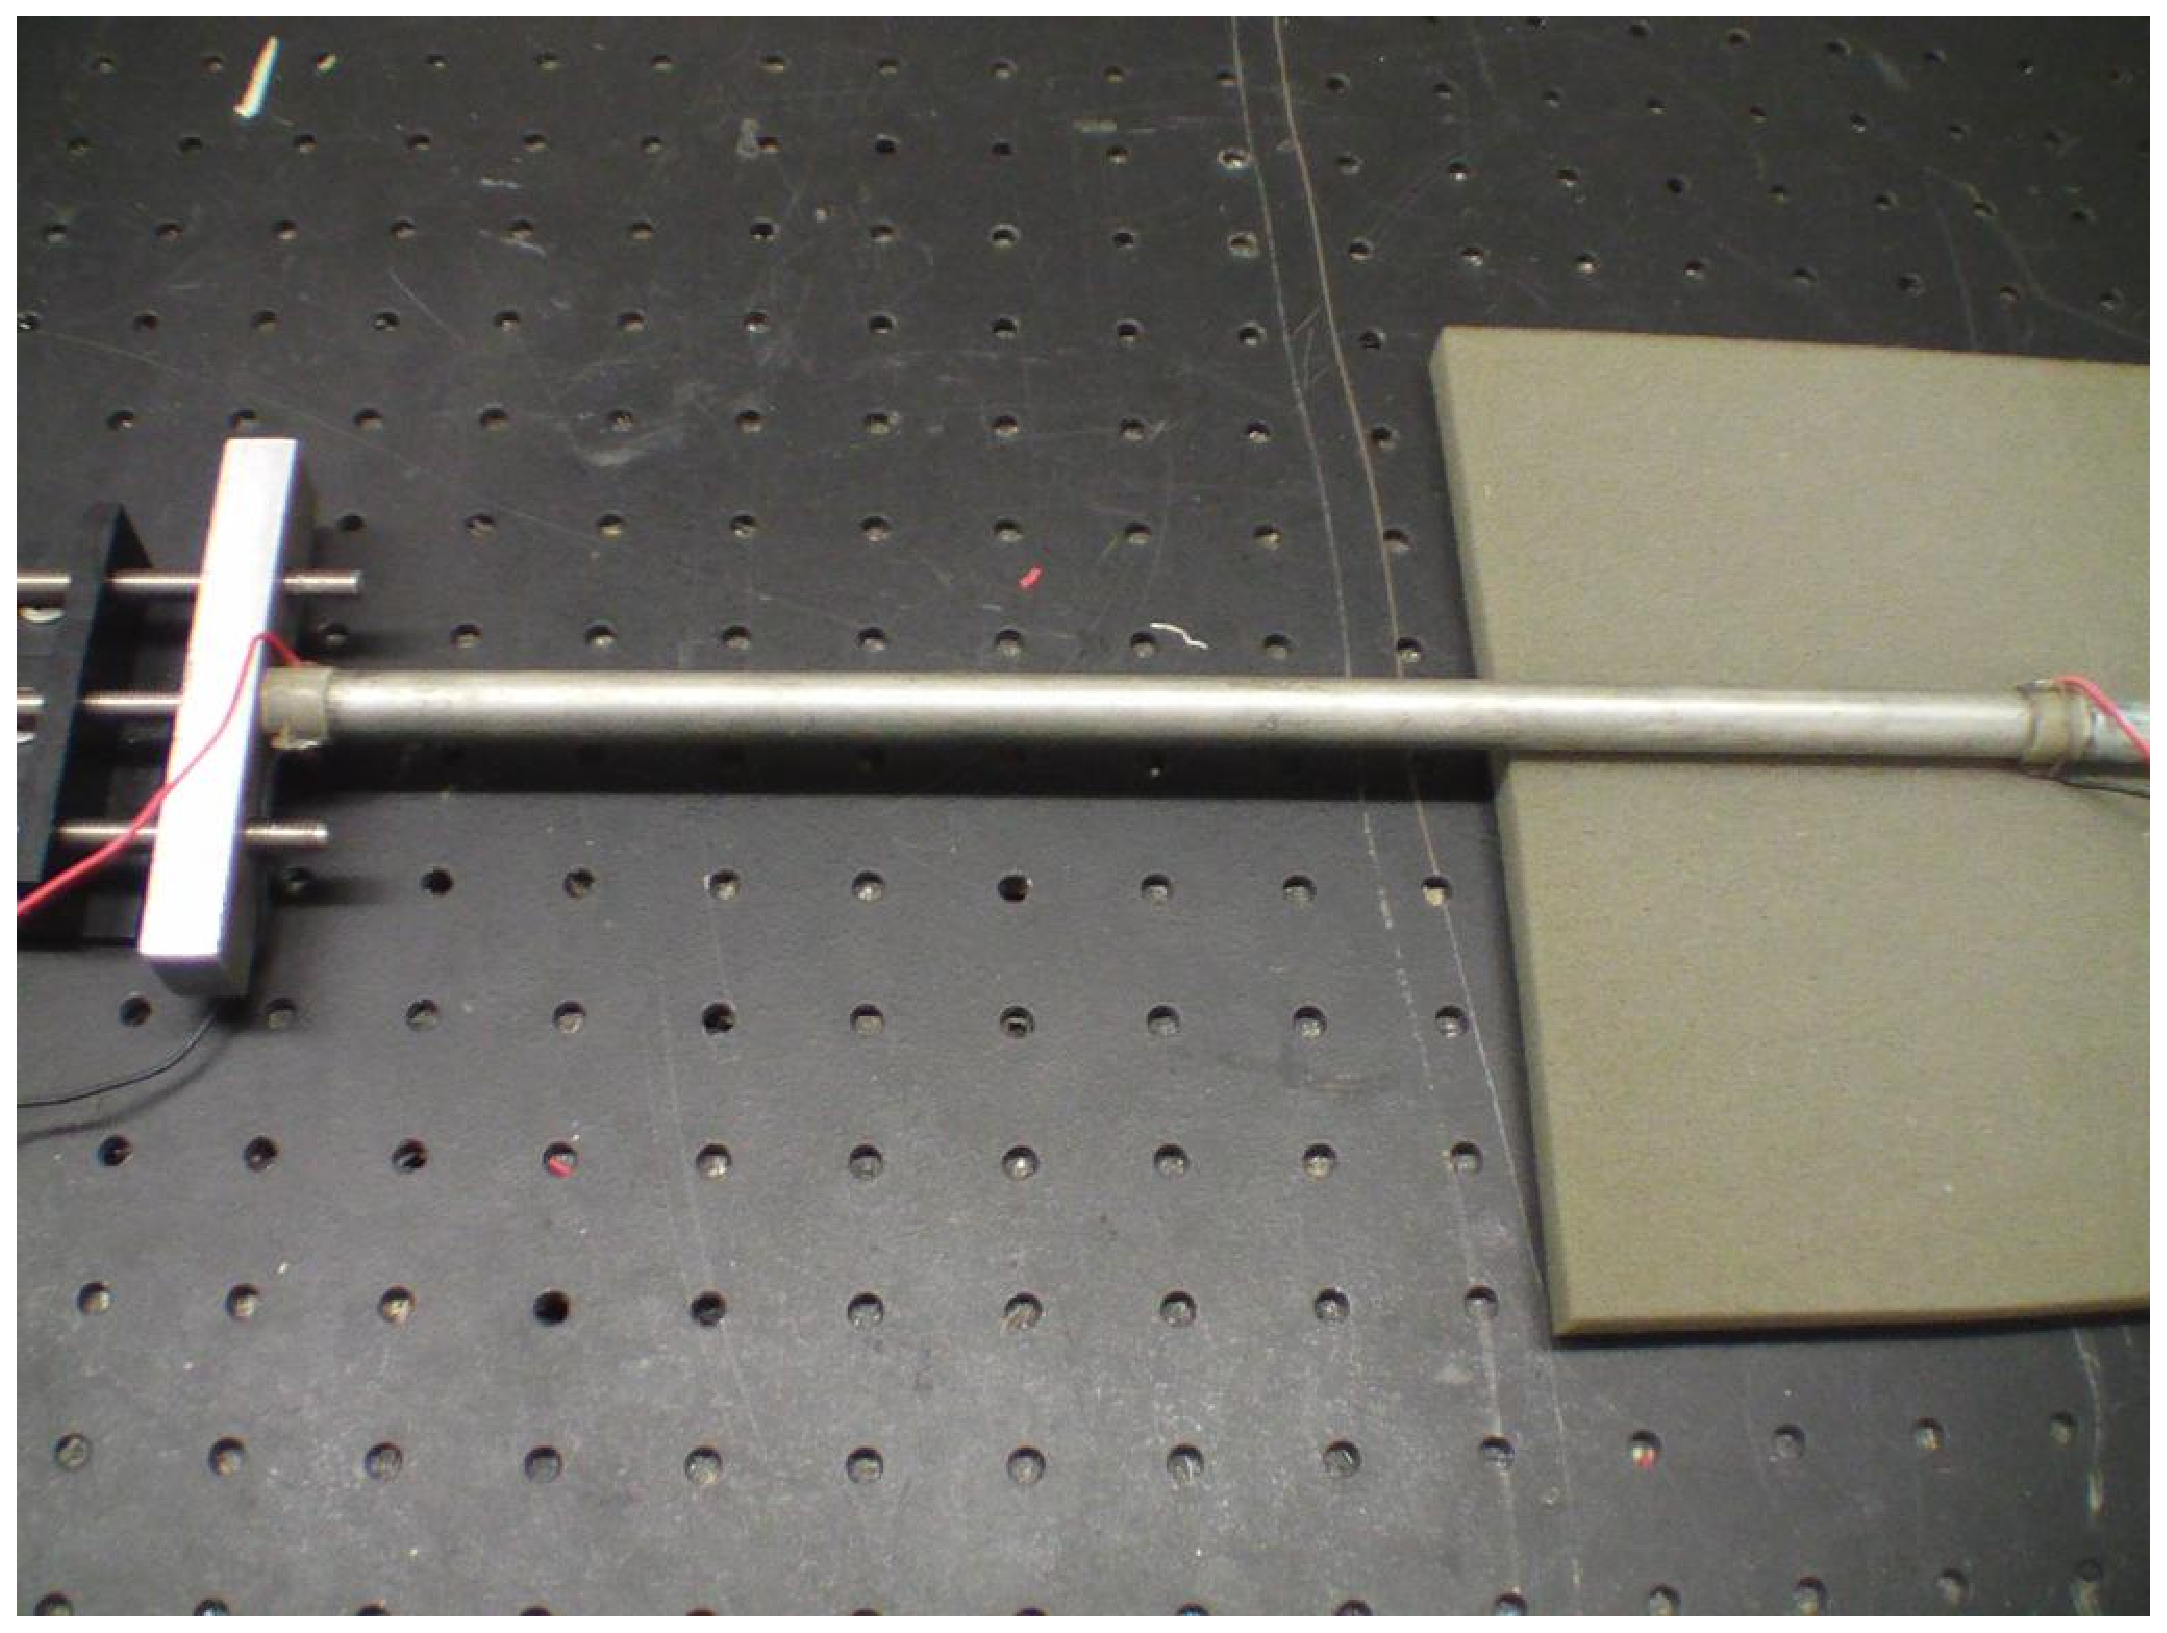
\includegraphics[width=9.7cm,height=5.75cm]{self_healing_setup2.eps}}
\end{subfigmatrix}
 %  \begin{center}
%   \begin{tabular}{c}
%   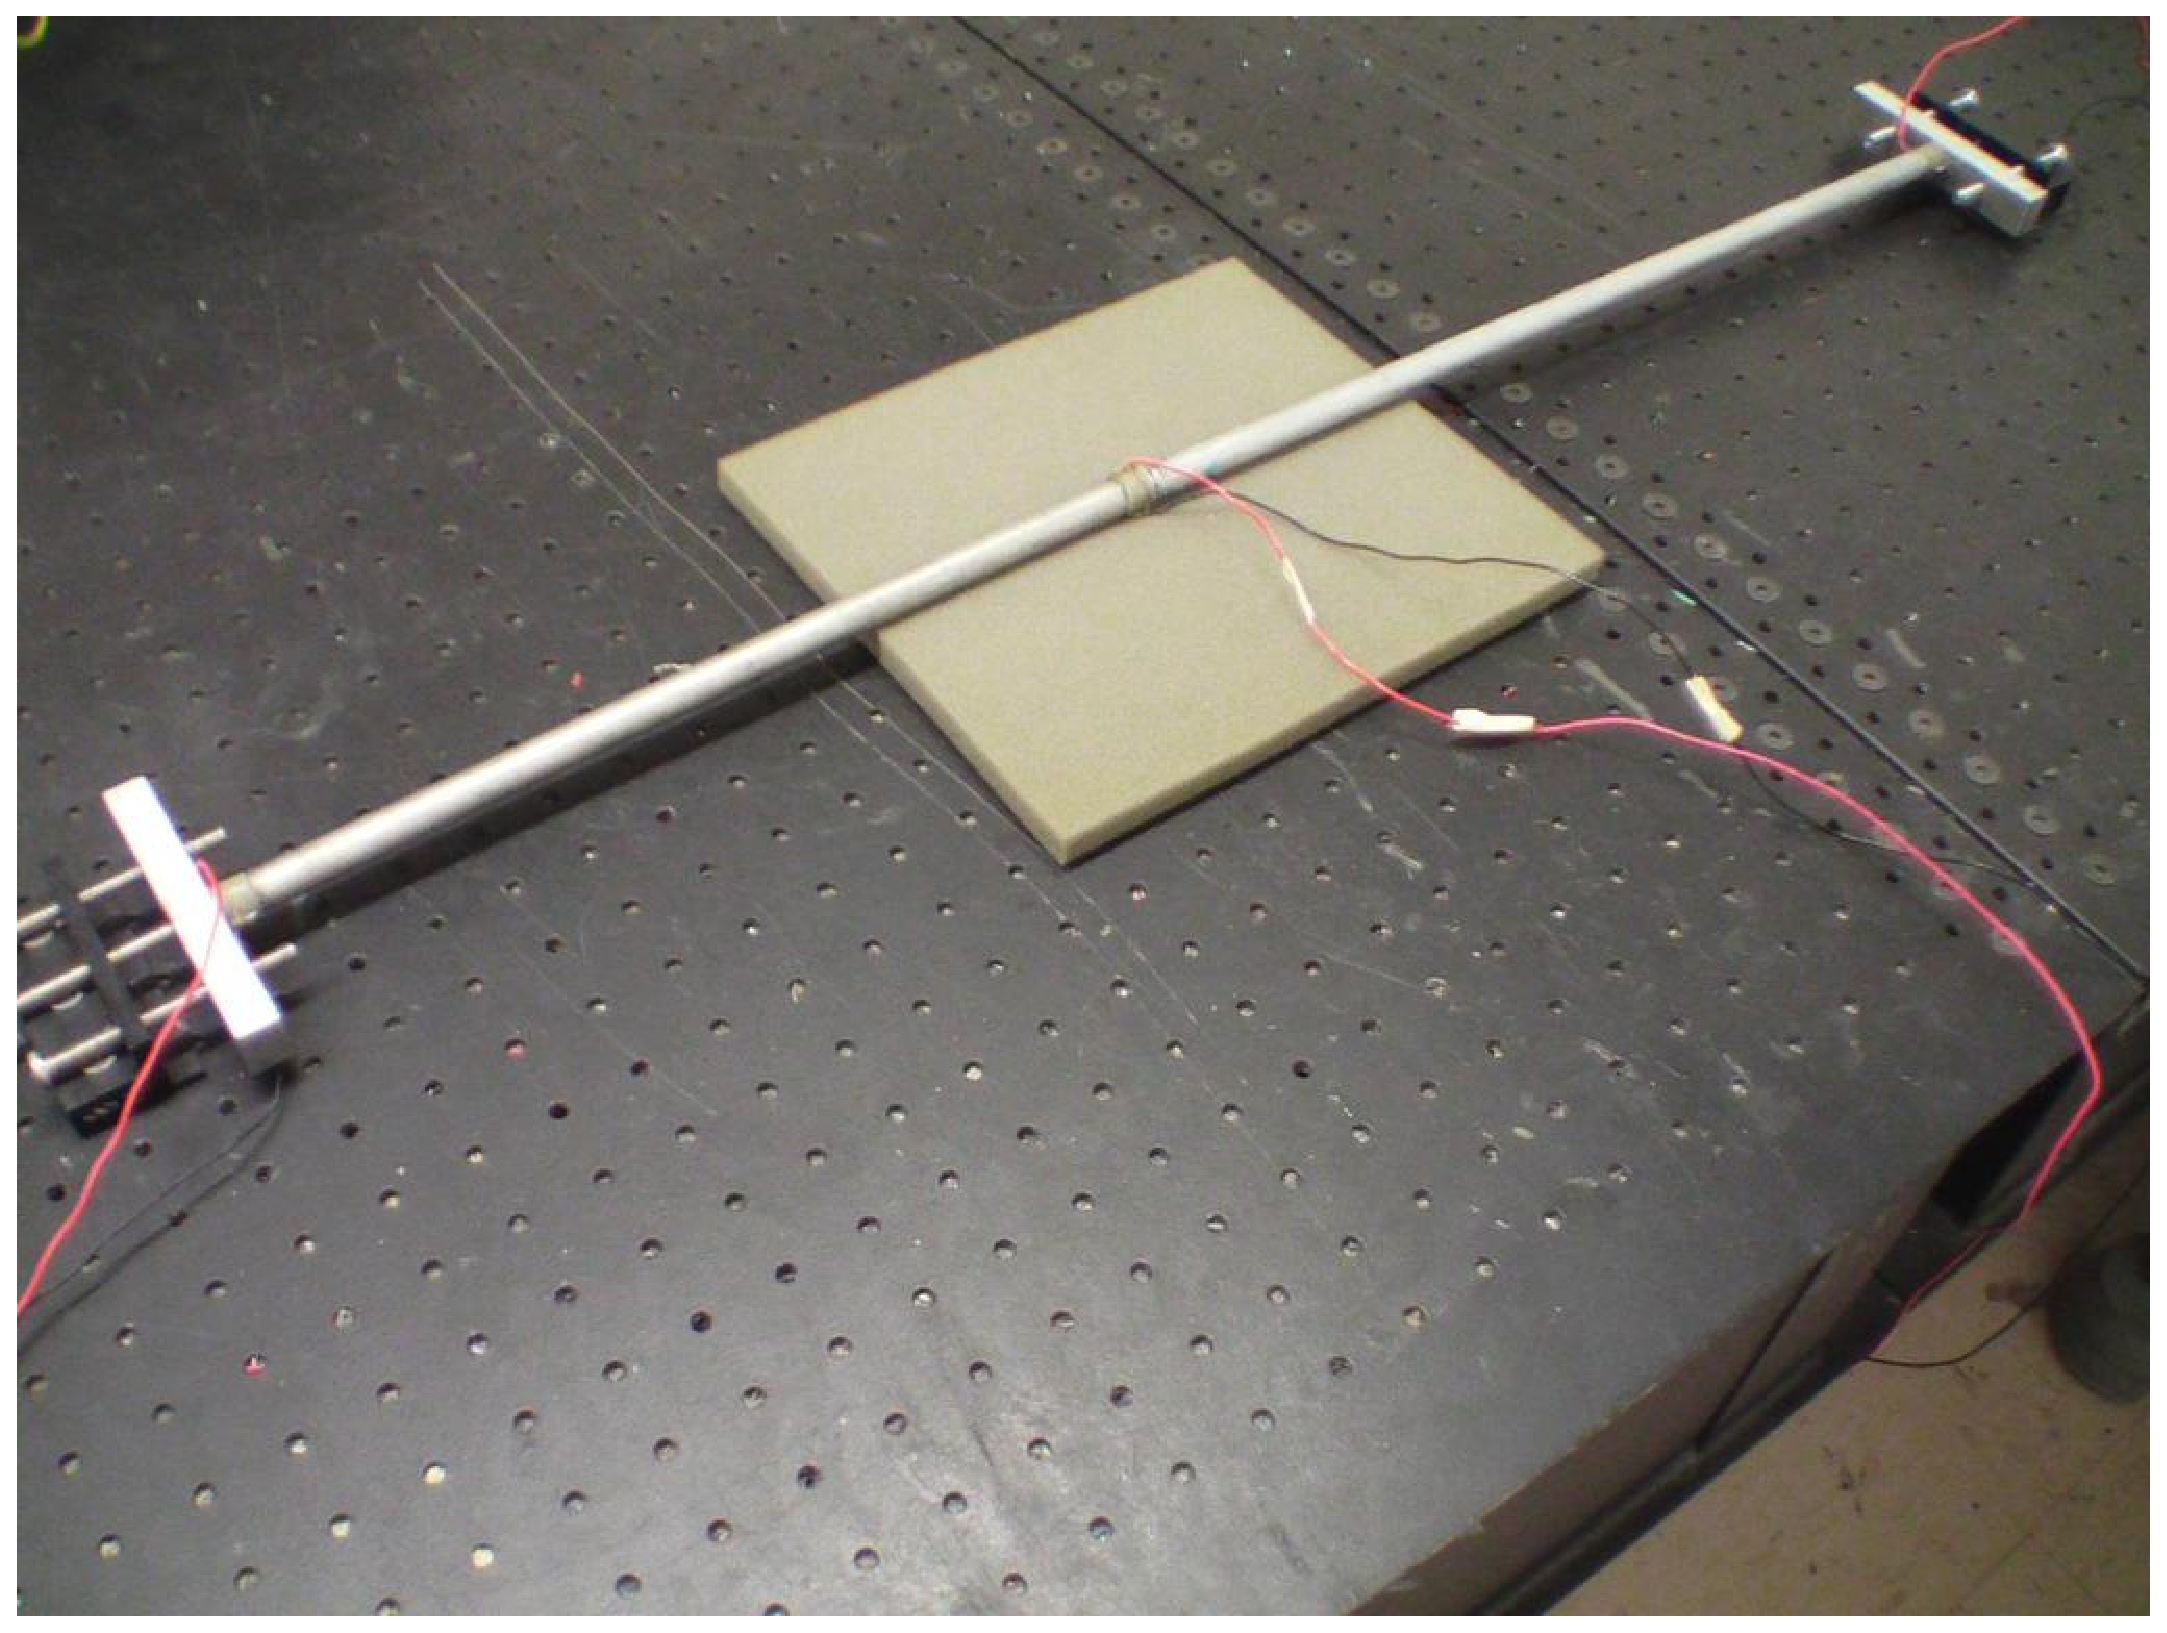
\includegraphics[height=5cm]{self_healing_setup1.eps}
%   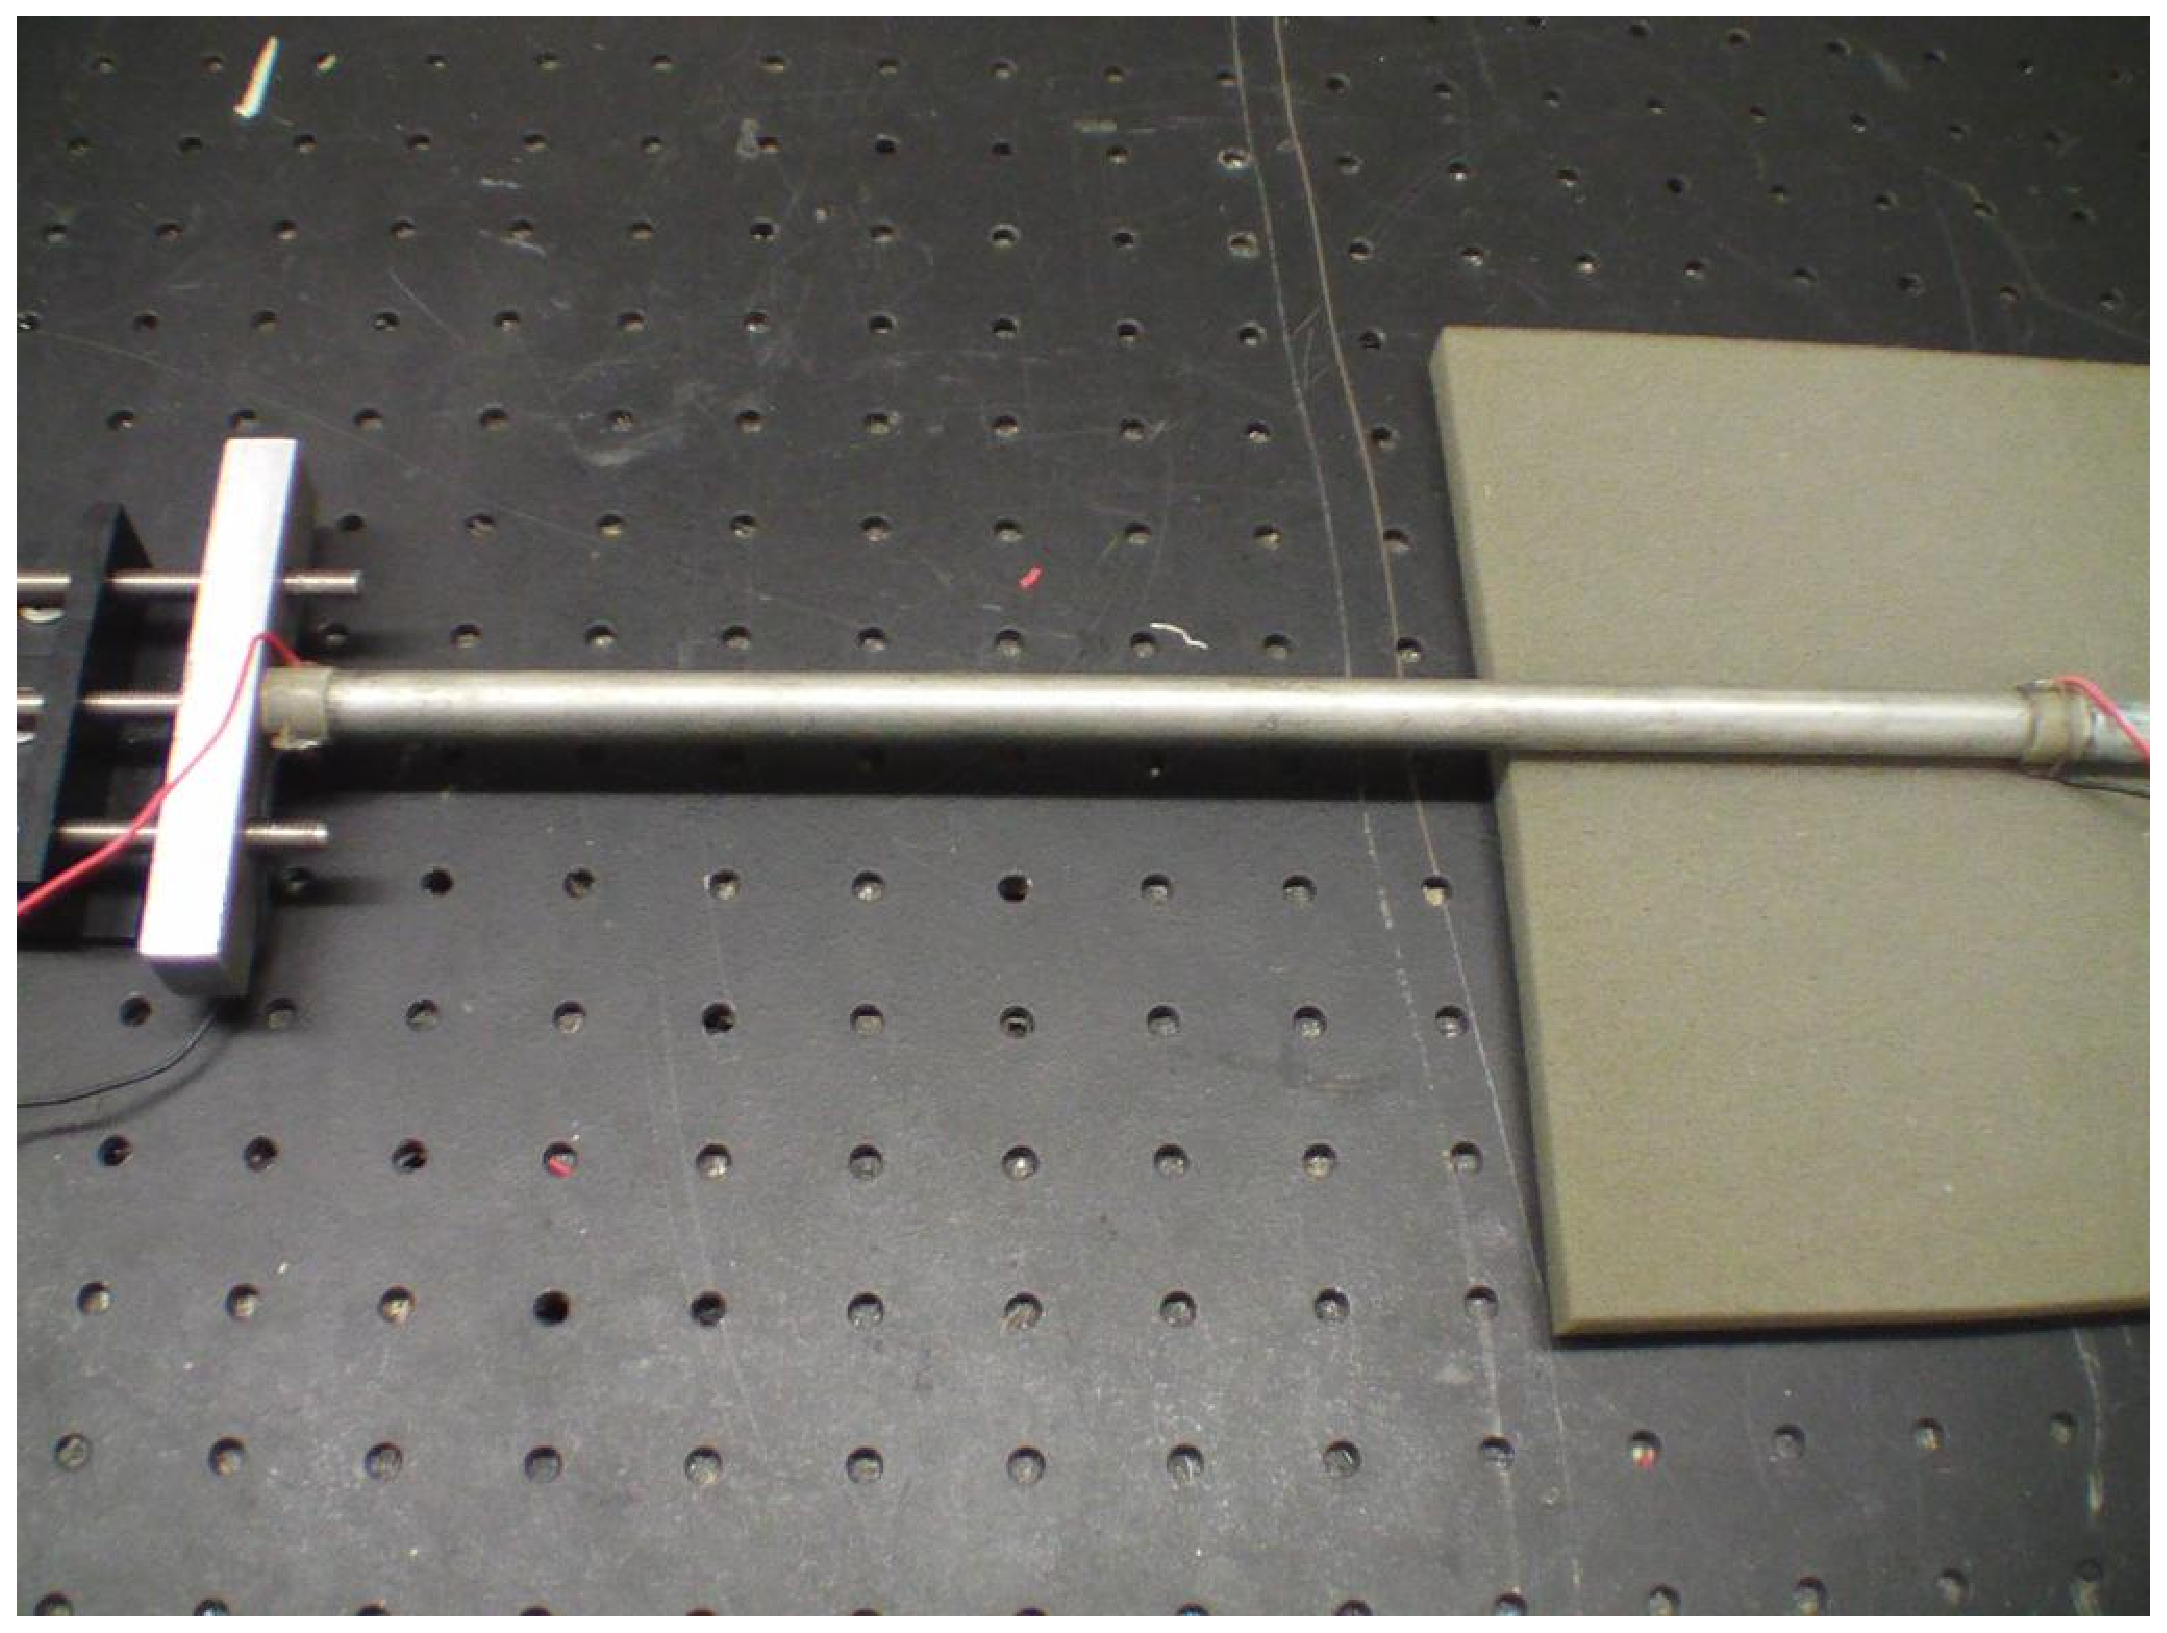
\includegraphics[height=5cm]{self_healing_setup2.eps}
%
%   \end{tabular}
%   \end{center}
   \caption[all]
%>>>> use \label inside caption to get Fig. number with \ref{}
   { \label{tr_setup_2}
(a) Overview of one set of steel rods that were used;
(b) Close up view of the right side steel rod (short rod).
The PZT seen on the left in (b) was the defect PZT and the PZT seen on the
right in (b) was PZT B.
 }
   \end{figure}
   
   \begin{figure}
\begin{subfigmatrix}{2}
\subfigure[Overview of Nylon Rod Apparatus]
{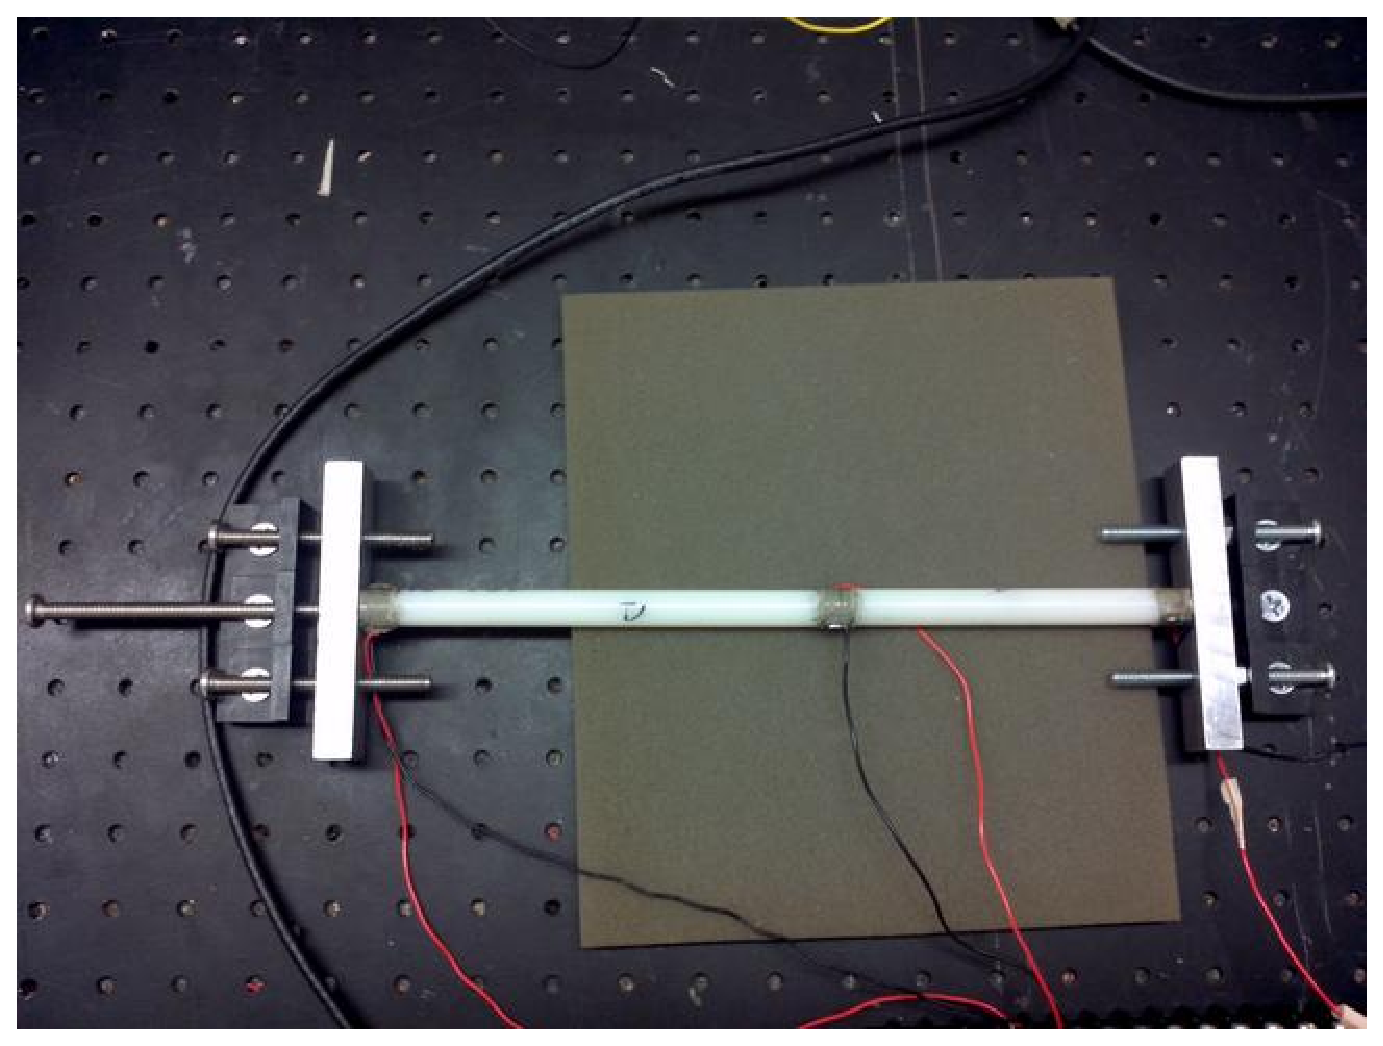
\includegraphics[width=9.7cm,height=5.75cm]{tr_setup_3.eps}}
\subfigure[Closer View of Apparatus]
{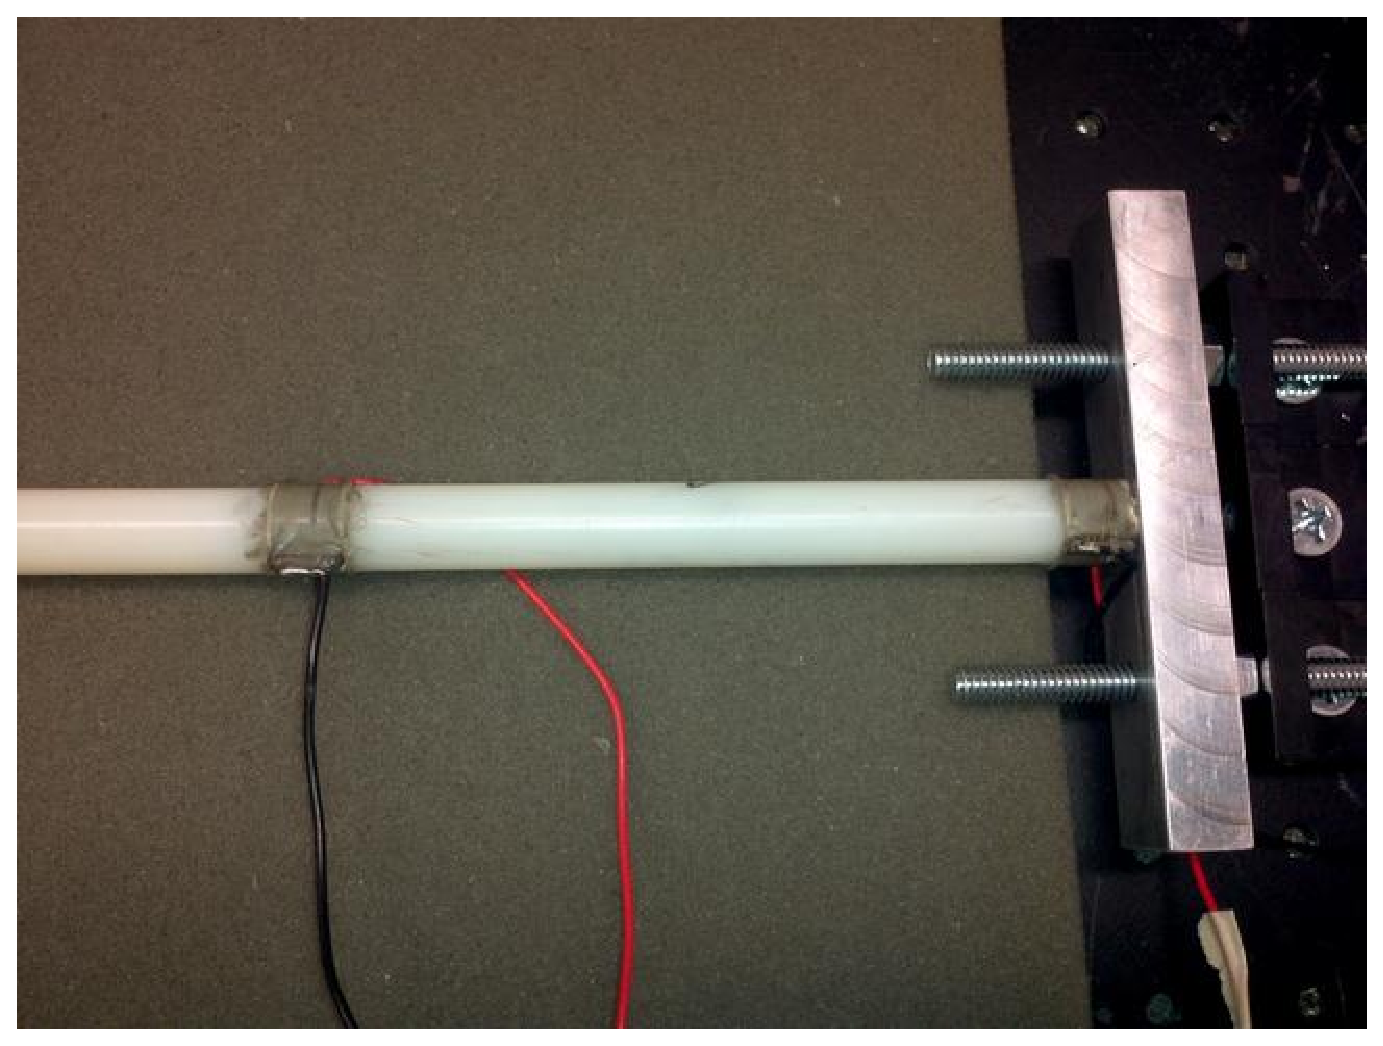
\includegraphics[width=9.7cm,height=5.75cm]{tr_setup_4.eps}}
\end{subfigmatrix}
 %  \begin{center}
%   \begin{tabular}{c}
%   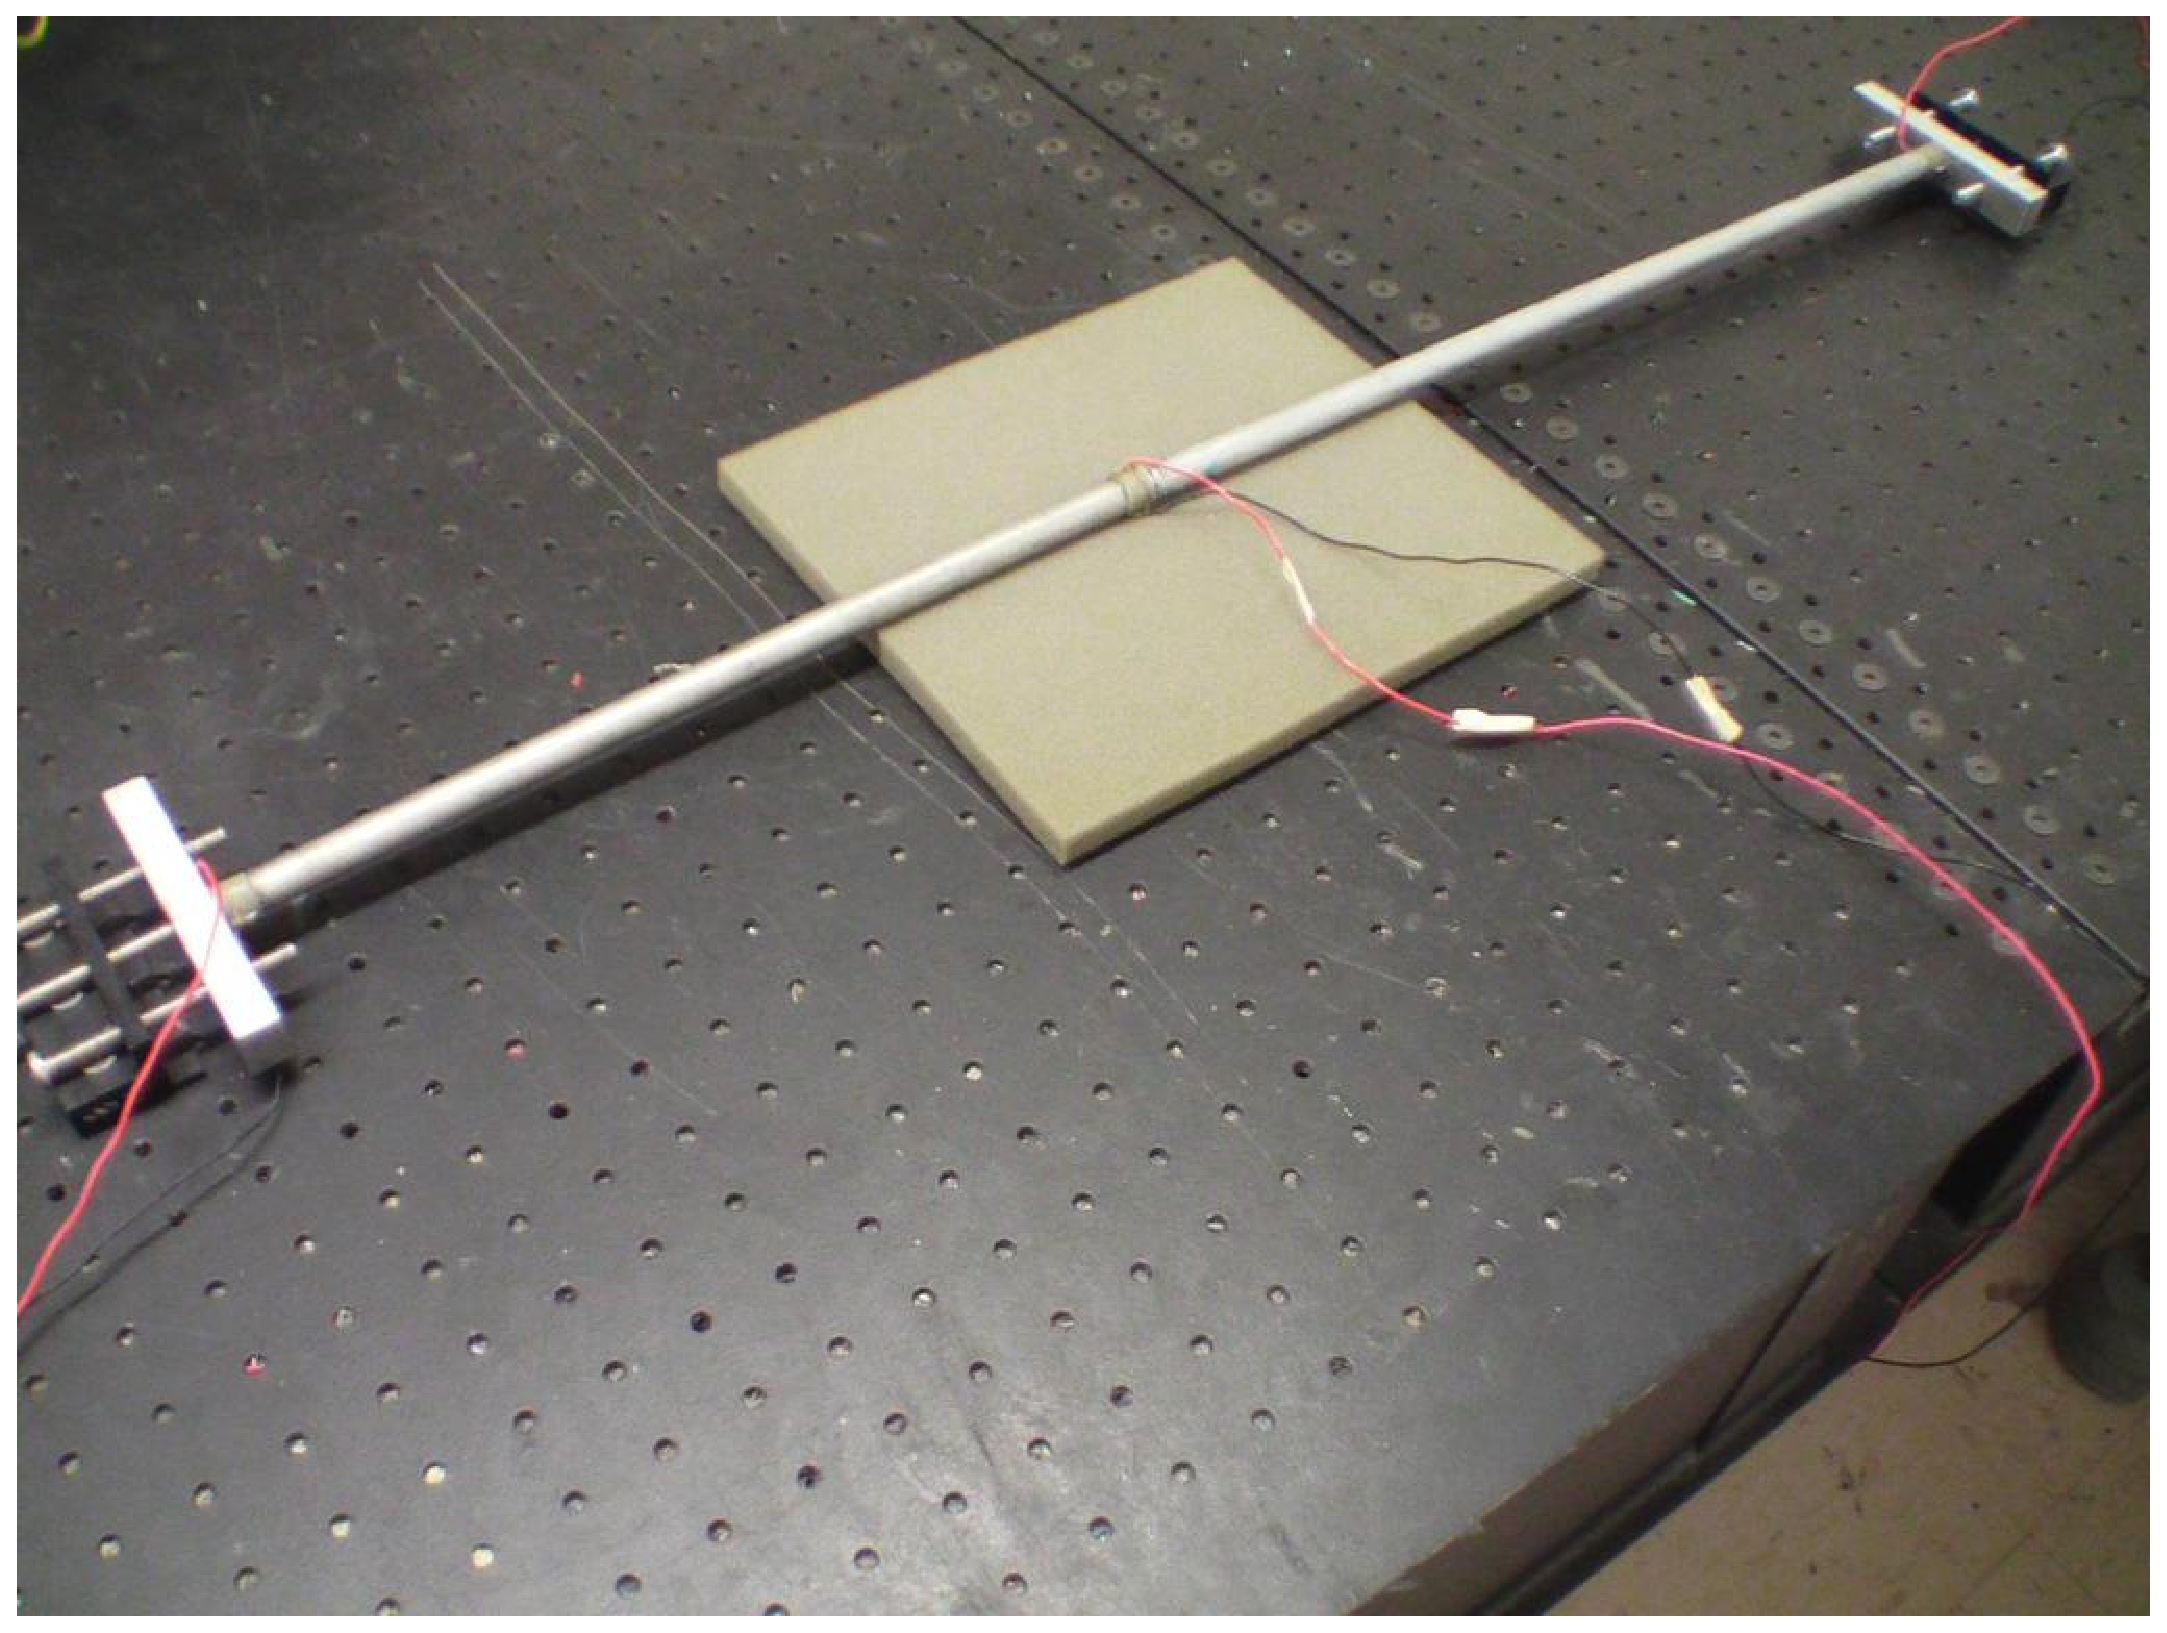
\includegraphics[height=5cm]{self_healing_setup1.eps}
%   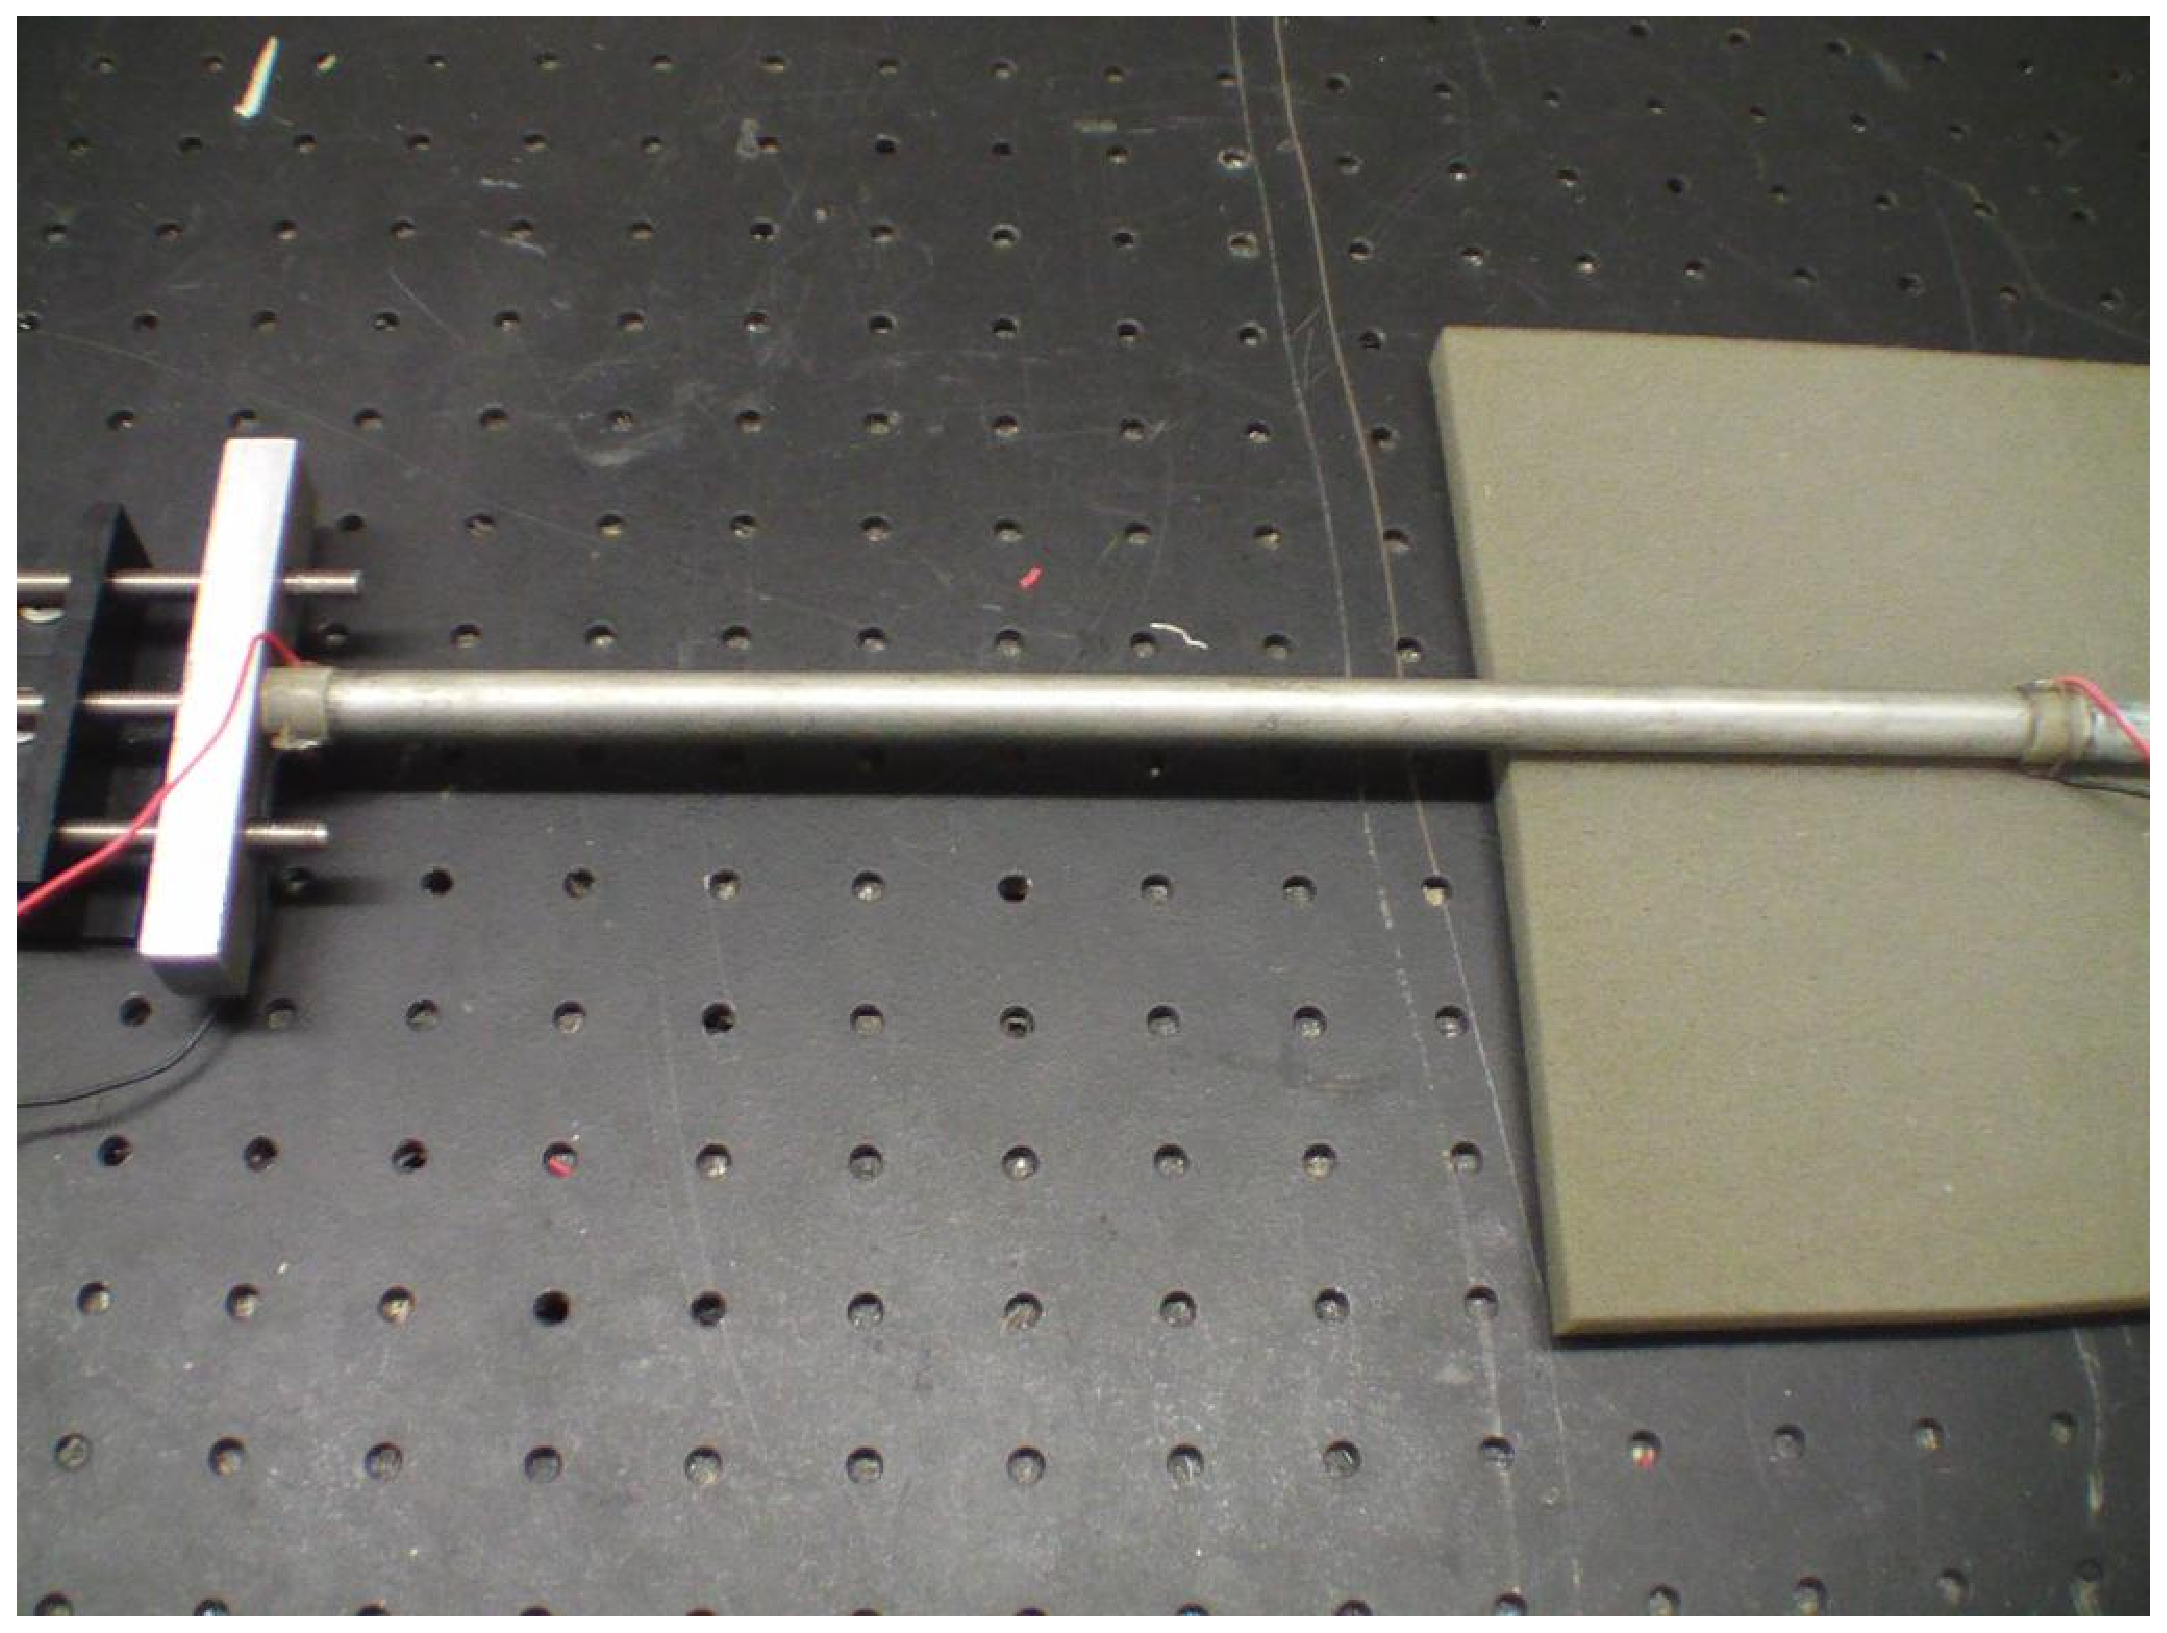
\includegraphics[height=5cm]{self_healing_setup2.eps}
%
%   \end{tabular}
%   \end{center}
   \caption[all]
%>>>> use \label inside caption to get Fig. number with \ref{}
   { \label{tr_setup_3}
(a) Overview of one set of nylon rods that were used;
(b) Close up view of the right side nylon rod (short rod) showing the defect transducer (left) and PZT B (right).
 }
   \end{figure}

\subsection{Hardware and Software Used}
\label{hardware}

A desktop PC running Windows XP was the main access point to the system. This PC was used to program and communicate with a National Instruments 7853R FPGA card. This card was housed in a PXI chassis and linked to the desktop PC via MXI cable, with the PC containing a PCI-E card to accept the MXI connection. Programs were written and compiled on the PC using LabVIEW, then downloaded to the FPGA card via the MXI connection. A host program ran on the PC and communicated with the program that ran on the FPGA card. The PC performed operations that were not time critical, whereas the FPGA card processed real time analog signals to and from the PZTs. The output signals from the FPGA card were amplified using op-amp amplifier circuits that were capable of providing $30$ VPP at $200$ kHz. All of the data acquisition cables were interfaced to the FPGA card by an SCH-60 shielded input/output box (Figure \ref{hardwareDiag}). The experimental results were imported into MATLAB.

\begin{figure}
\begin{center}
{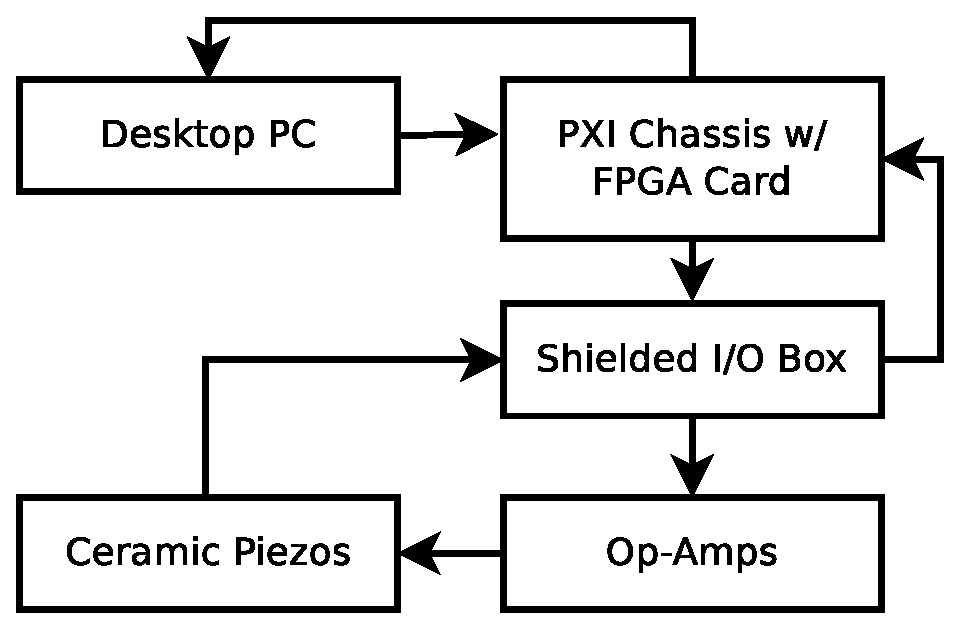
\includegraphics[width=9.7cm,height=4cm]{hardwareComm.eps}}
 \caption[comp1]
%>>>> use \label inside caption to get Fig. number with \ref{}
   { \label{hardwareDiag}
   Simple diagram showing the communications hierarchy among the different pieces of hardware that were used for the time reversal testing. The desktop PC and PXI/FPGA communicated over an MXI cable. The FPGA card interfaced to the I/O box using a proprietary shielded cable. All other connections were made using commonly available insulated copper wire.
 }
 \end{center}
 \end{figure}

\subsection{Time Reversal Signal Processing Algorithm}
\label{trAlgorithm}
The software consisted of two main programs, the host program and the FPGA program. As the names imply, the host program ran on the desktop PC and the FPGA program executed on the FPGA card. The host code was launched first, at which point a new FPGA program was downloaded to the FPGA card and executed. All communication between the host program and the FPGA program was done using the FGPA's on board First-In-First-Out memory (FIFO) to which the host program had direct memory access (DMA). A handshaking protocol implemented by IRQs was used to synchronize data transactions between the host and FPGA programs.

The LabVIEW software was used to generate an initial multi-tone wave that was sent out by one of the PZTs. This wave was created by first generating individual, single period sine waves of different frequencies. These individual waves were then concatenated together to form the overall multi-tone wave. The center frequency chosen for this test was $115$ kHz with a bandwidth of $30$ kHz. The frequencies of the waves were obtained by relating the number of points used to create the waves with the sampling frequency of the FPGA card that played the waves ($740.741$ kHz here). For the $130$, $115$, and $100$ kHz waves the program used $7$, $8$, and $9$ data points, respectively, to represent a single sinusoidal period of those frequencies. The $130$ kHz wave was placed in the middle of the wave group, with a $115$ kHz wave to either side of it and a $100$ kHz wave on the ends of those (Figure \ref{initialWave}). The multi-tone wave was found to provide better response amplitudes during testing than single frequency waves. This could be due to the excitation of more modes in the medium.

\begin{figure}
\begin{center}
{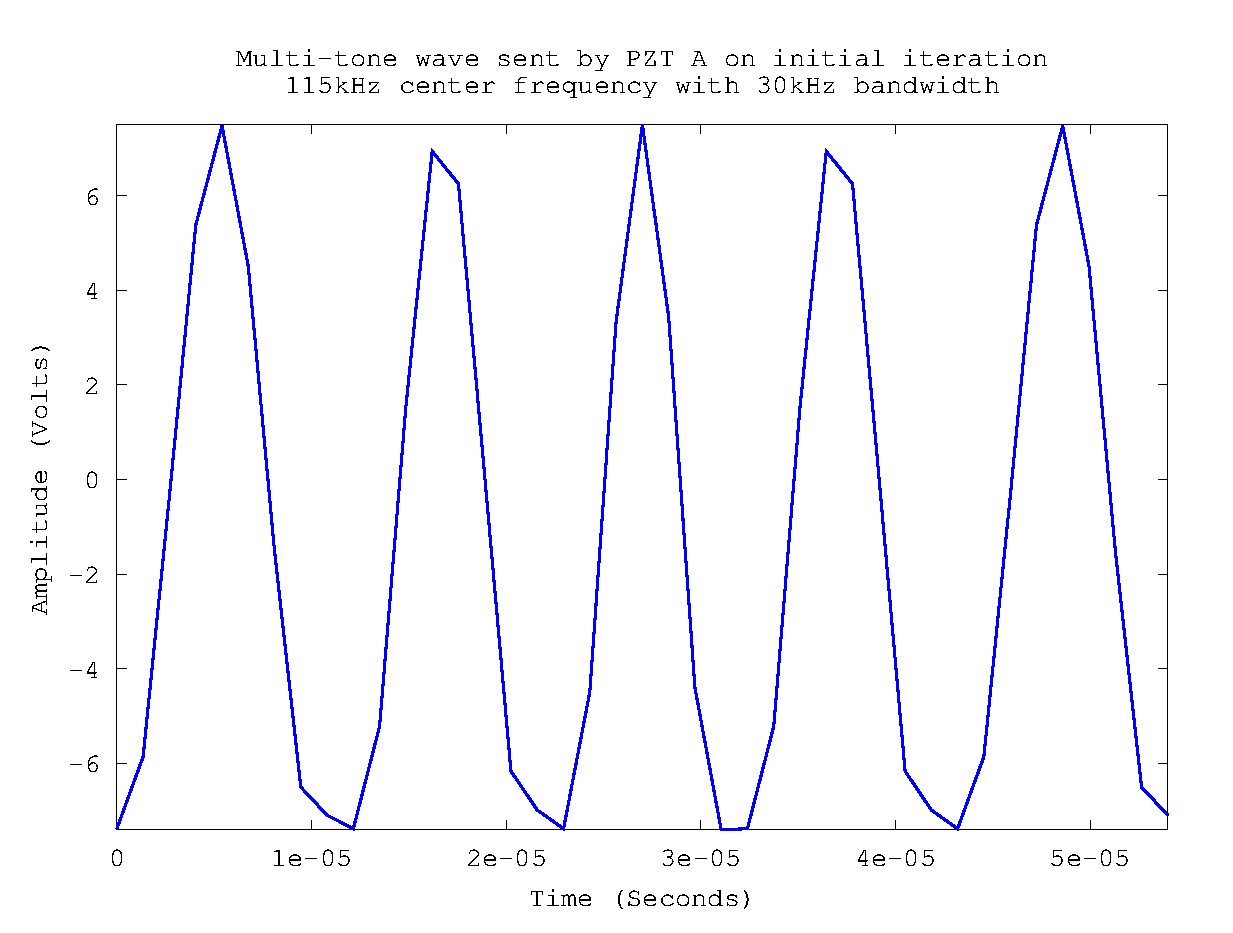
\includegraphics[width=9.7cm,height=5.75cm]{initialWave.eps}}
 \caption[comp1]
%>>>> use \label inside caption to get Fig. number with \ref{}
   { \label{initialWave}
   Multi-tone wave that was initially played out by PZT A. This wave was constructed of multiple single period sinusoidal waves. The peak seen in the middle is a $130$ kHz wave, the waves directly to its sides are $115$ kHz, and the waves on either end are $100$ kHz. Better response amplitudes have been seen during testing by using the multiple frequencies versus a single frequency.
 }
 \end{center}
 \end{figure}

The initial wave (along with program variables) was transmitted to the FPGA program which set all of its output values to zero and waited 200 ms. The wait time was chosen based on experimental observations for the decay time of a signal propagating through either a steel or nylon rod. After the wait time elapsed, the initial wave was sent from one of the end PZTs (A or B). The algorithm was indifferent to which PZT played the initial wave. PZT A played the initial wave and simultaneously began to record. The defect PZT and PZT B also began recording as soon as PZT A began playing. The initial wave propagated through the rod and struck the defect PZT. Upon impacting the defect PZT, the initial wave split into a reflected component and a transmitted component. The reflected component traveled back towards PZT A and was recorded. The transmitted component approached PZT B where it was recorded. These components were reflected back and forth between the transducers a number of times more and each reflection was recorded by the PZTs in the setup (Figure \ref{initRead}). This continued until the specified number of samples to take was reached (2000 samples was chosen here based upon experimental observations).

\begin{figure}
\begin{subfigmatrix}{2}
\subfigure[PZT A Recorded Response]
{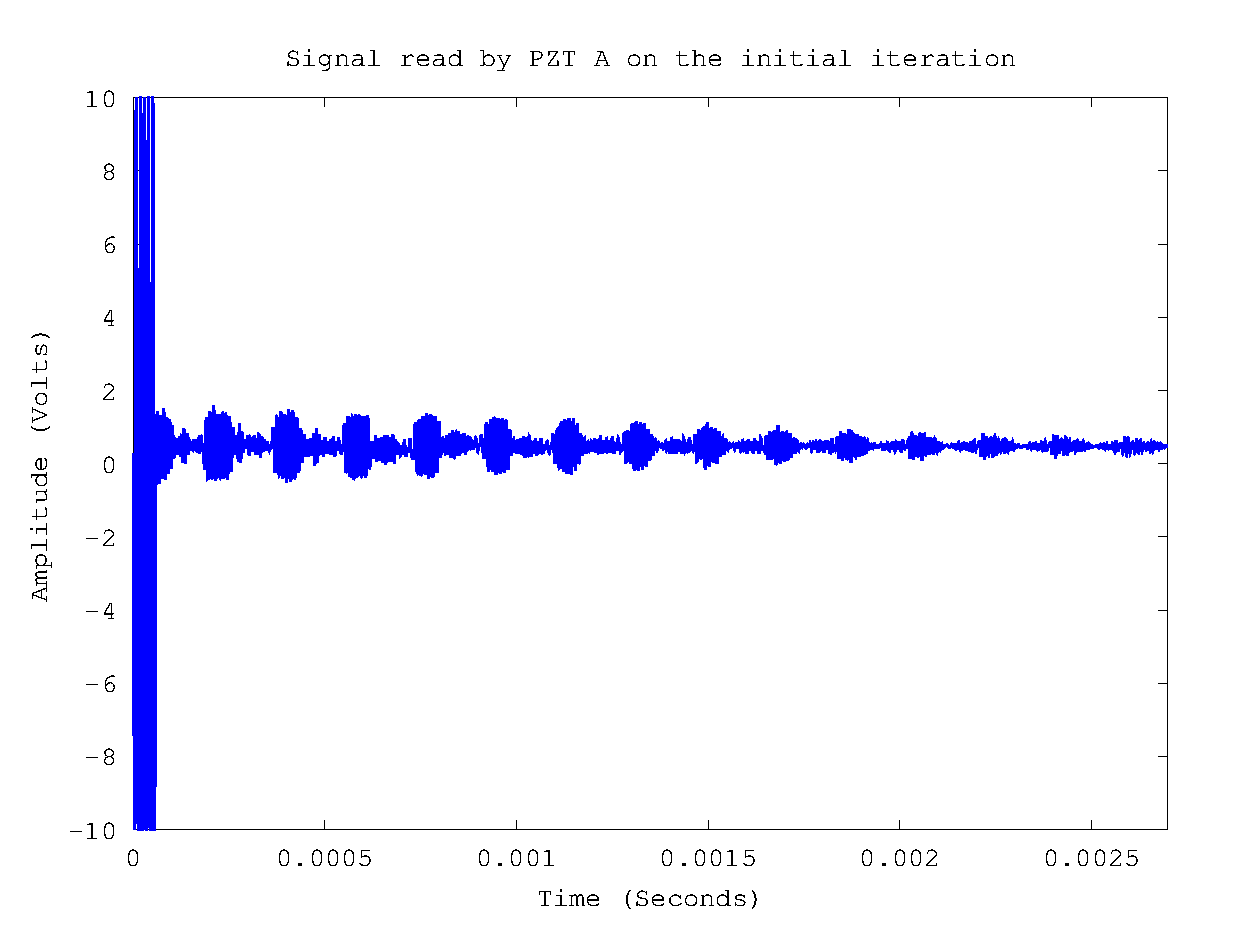
\includegraphics[width=9.7cm,height=5.75cm]{ch0Read.eps}}
\subfigure[PZT B Recorded Response]
{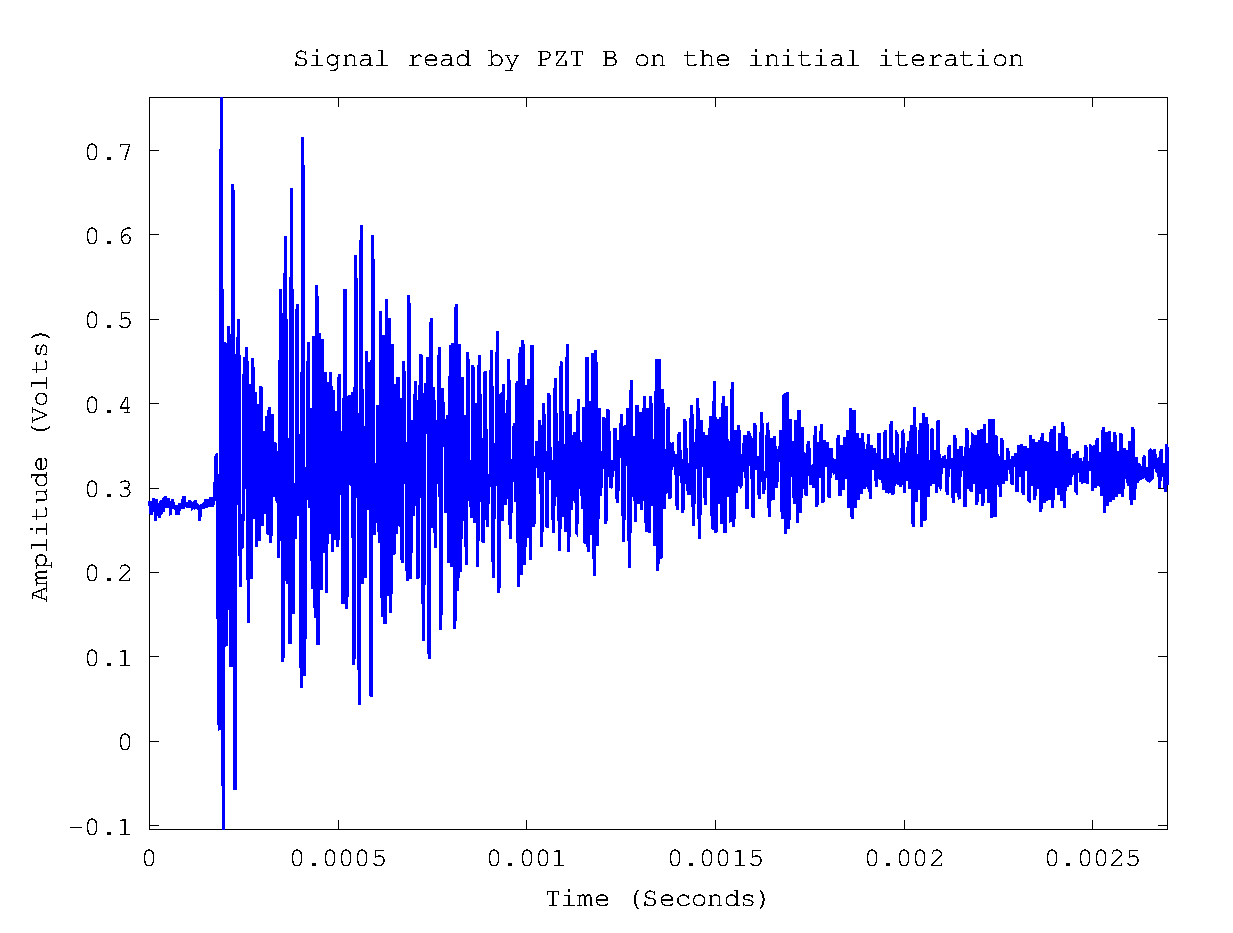
\includegraphics[width=9.7cm,height=5.75cm]{ch1Read.eps}}
\end{subfigmatrix}
 %  \begin{center}
%   \begin{tabular}{c}
%   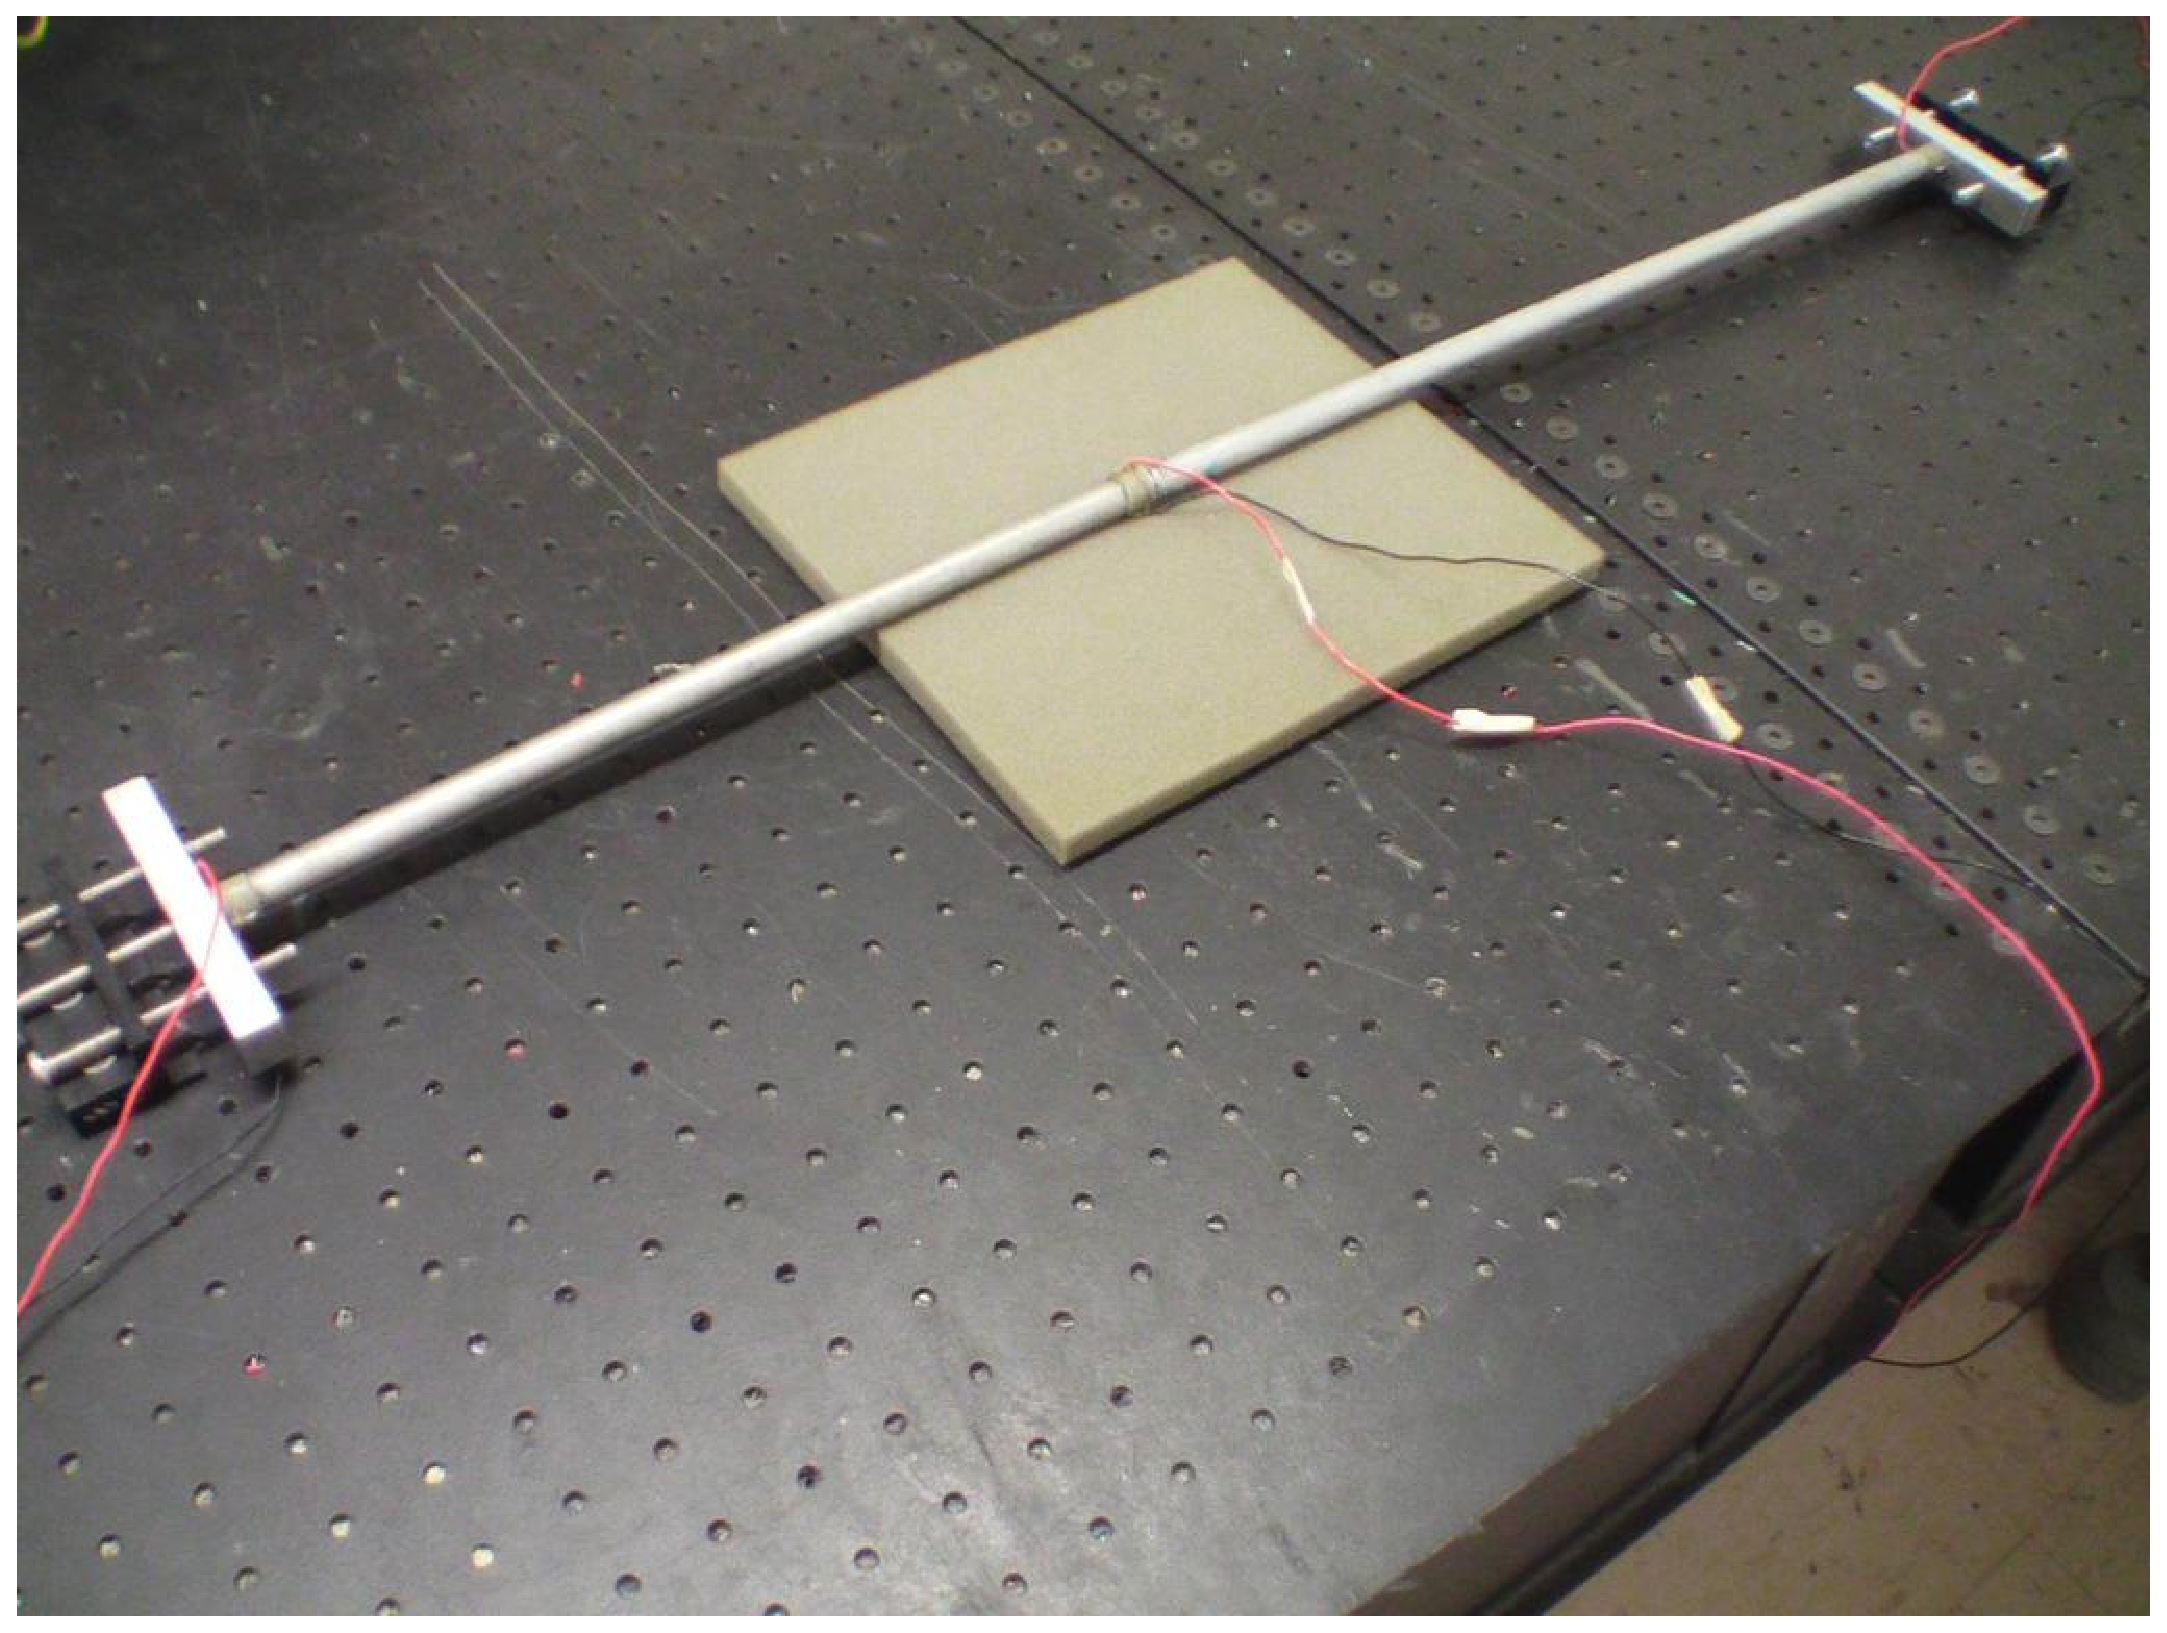
\includegraphics[height=5cm]{self_healing_setup1.eps}
%   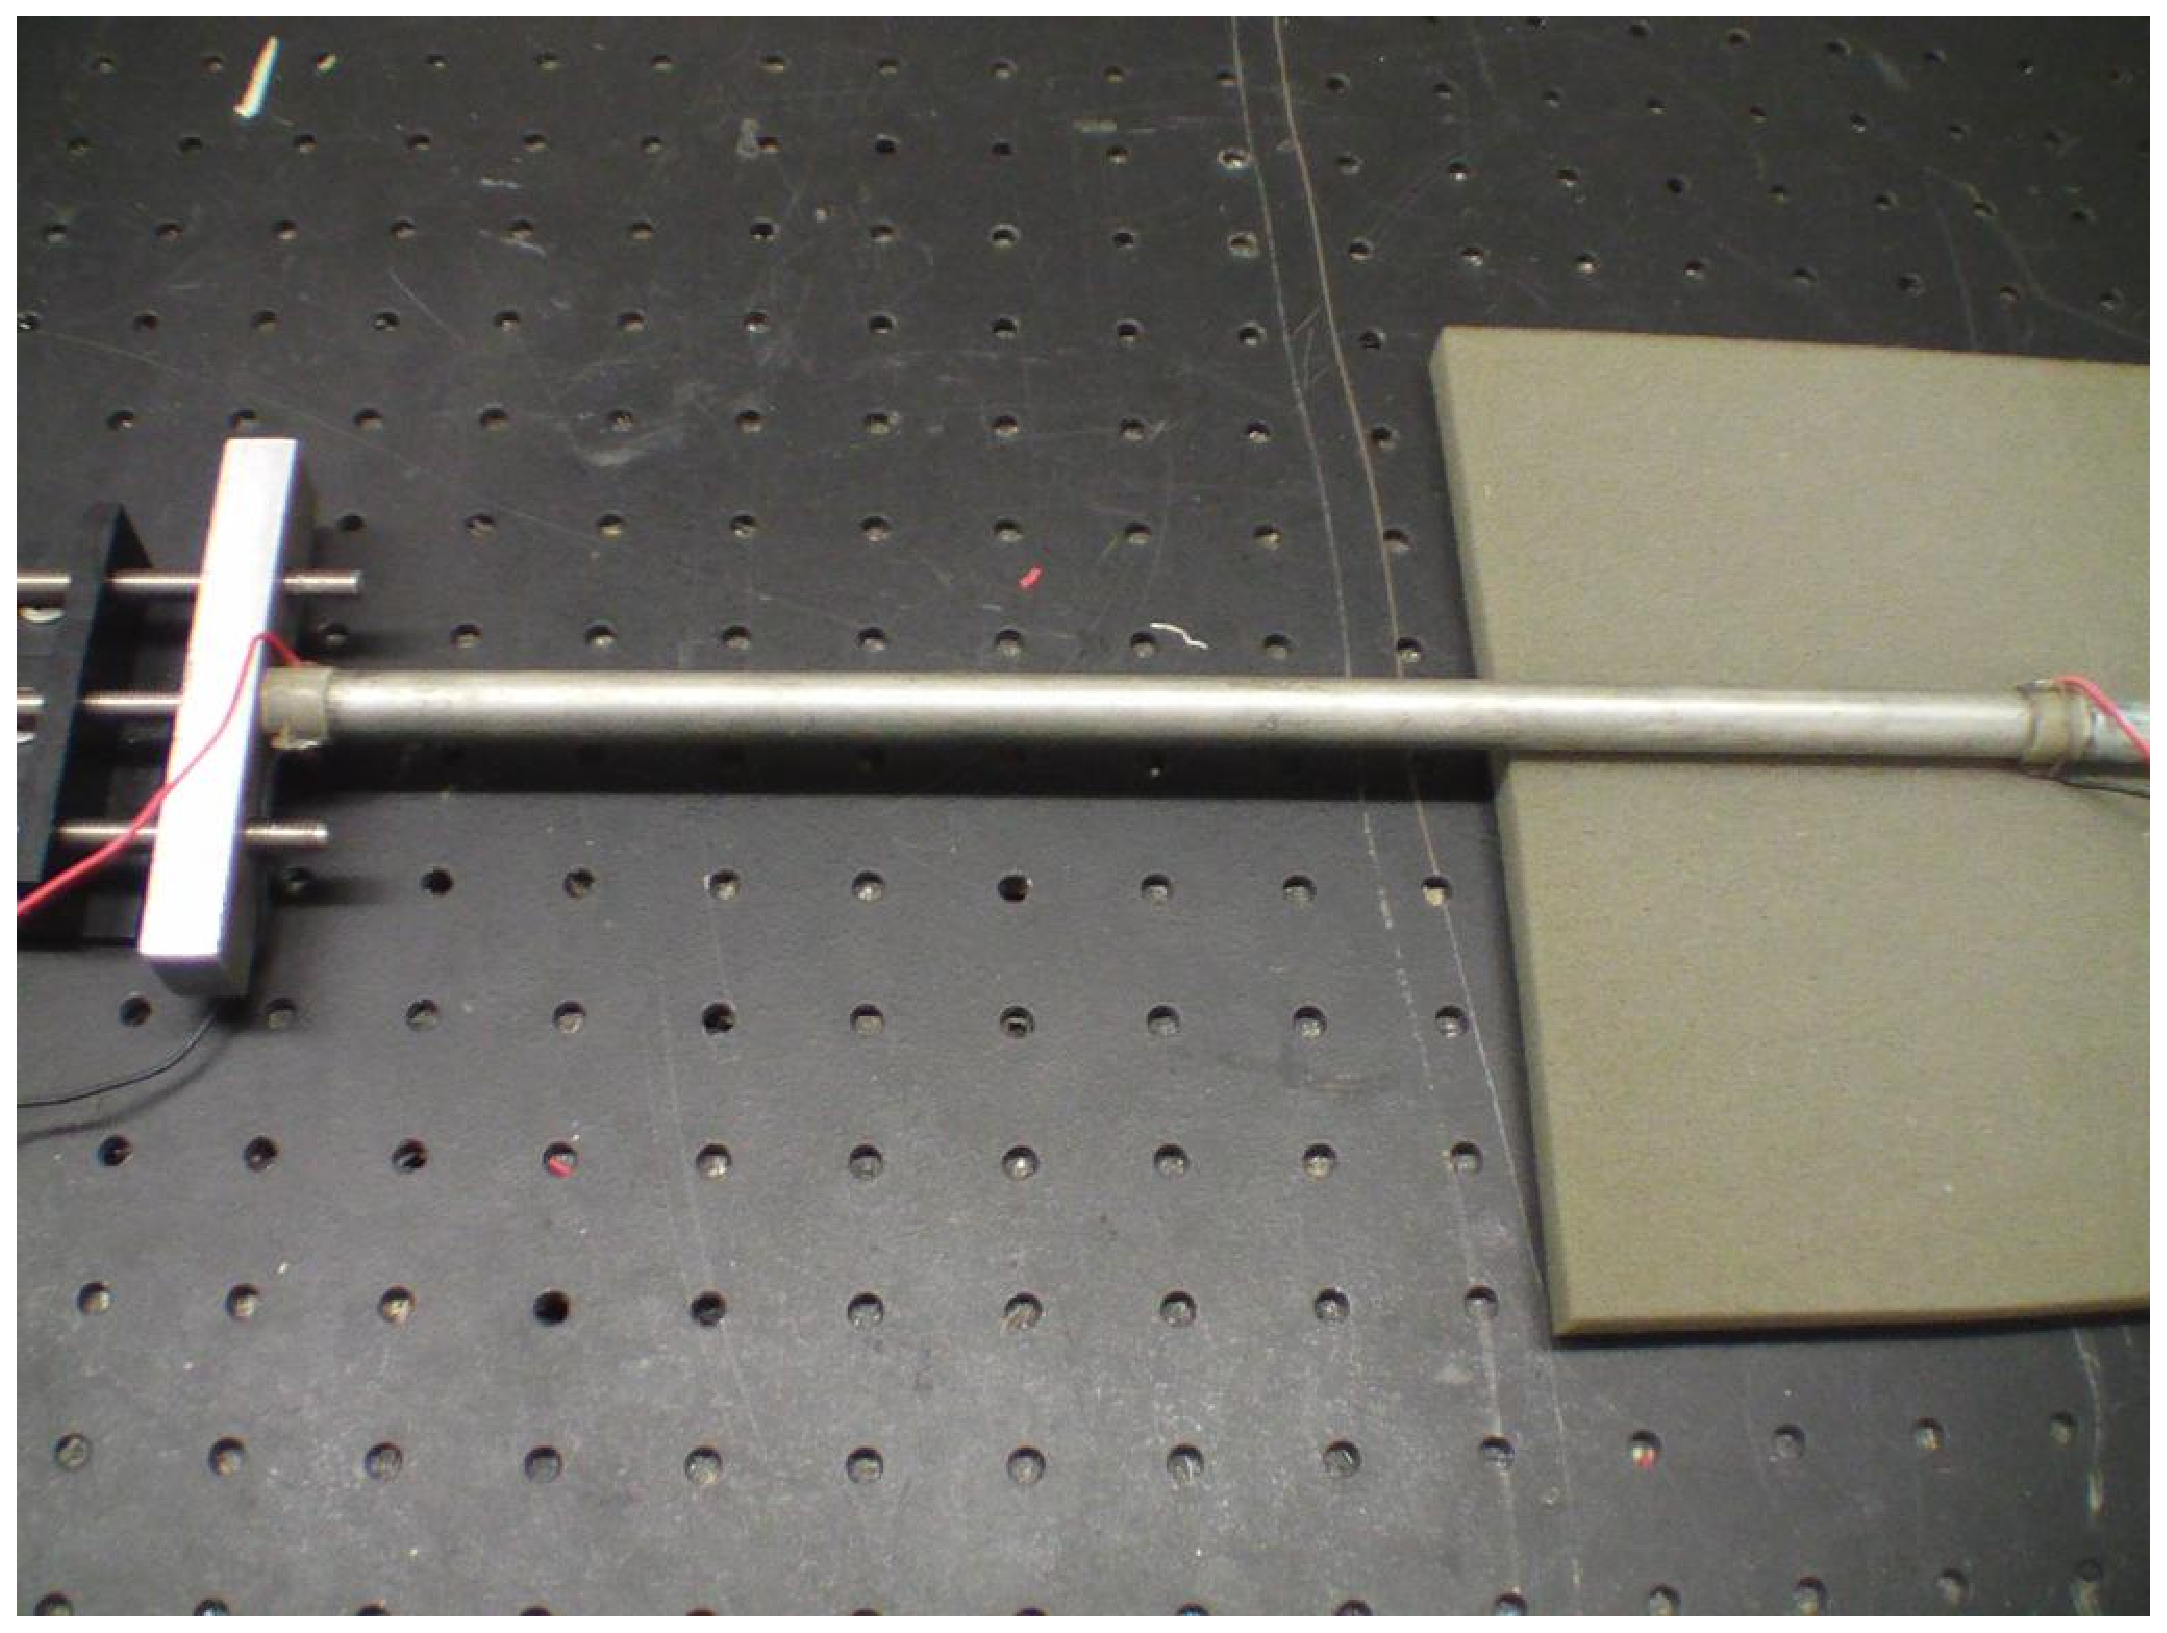
\includegraphics[height=5cm]{self_healing_setup2.eps}
%
%   \end{tabular}
%   \end{center}
   \caption[all]
%>>>> use \label inside caption to get Fig. number with \ref{}
   { \label{initRead}
(a) Response recorded by PZT A (sender) during the initial iteration. These tests were performed on the steel rods of length $437$ mm and $428$ mm. Notice that the initial wave that PZT A played out was recorded in its signal and was much greater in amplitude than the reflection waves seen in the recorded signal. This was one difficulty when performing time reversal in one dimension. When attempting to determine which time window to play back during the time reversal iterations, it was necessary to zero out this first section and also bypass any transient ringing left over from playing out the initial wave;
(b) Response recorded by PZT B (opposite end) during the initial iteration.
 }
   \end{figure}

After the specified number of samples were recorded, the data from each PZT were transferred from the FPGA program back to the host program for processing.\footnote{An enormous amount of the FPGA's limited program space was saved by using it only for time-critical processes.} The host program took the signal recorded by PZT A and performed a windowed root mean square (RMS) operation on it. A window size of 40 data points was used based on our initial wave size of 40 data points. The windowed RMS algorithm was as follows:

\begin{algorithmic}

\For{$i =1 \to signalLength - windowLength$}

$startRMS = i$

$endRMS = i + windowLength$

\%\% Subset function returns a subset of the given signal starting at startRMS and ending at endRMS \%\%

$signalSubset = subset( signal, startRMS, endRMS )$

\%\% Subtract the mean of signalSubset from itself so that the data becomes centered on zero\%\%

$signalSubset = signalSubset  - mean(signalSubset)$

\%\% Compute the RMS for the current window of the recorded signal \%\%

$windowedSignalRMS[ i ] = RMS( signalSubset ) $	

\EndFor

\end{algorithmic}

The output, windowedSignalRMS, was a graph that essentially drew a line around the wave groups that were recorded within the signal read by PZT A (Figure \ref{windowedRMS}). The peaks in this RMS plot corresponded to the time at which the highest concentrations of stress-wave energy occurred at PZT A as a result of the initial wave that was played out. Since PZT A played out a signal while it was recording data, it was important to zero out the data points during this time period so that they did not overshadow the reflections of the initial wave of interest (this is also mentioned in the caption for Figure \ref{initRead}). The period to zero out was specified at program start up. For these experiments, the first 100 data points read by the PZT were zeroed out which was a little more than twice the length of the initial 40 data point wave that was played out. After zeroing out the ringing from the PZT, the maximum peak that was seen in the RMS graph corresponded to the time that the reflection of the initial wave from the defect PZT first occurred at PZT A. This was the window from PZT A to reverse in our time reversal phase. An identical procedure was used on the signal read by PZT B to find the first occurrence at PZT B of the transmitted component of the initial wave.

\begin{figure}
\begin{subfigmatrix}{2}
\subfigure[PZT A Windowed RMS]
{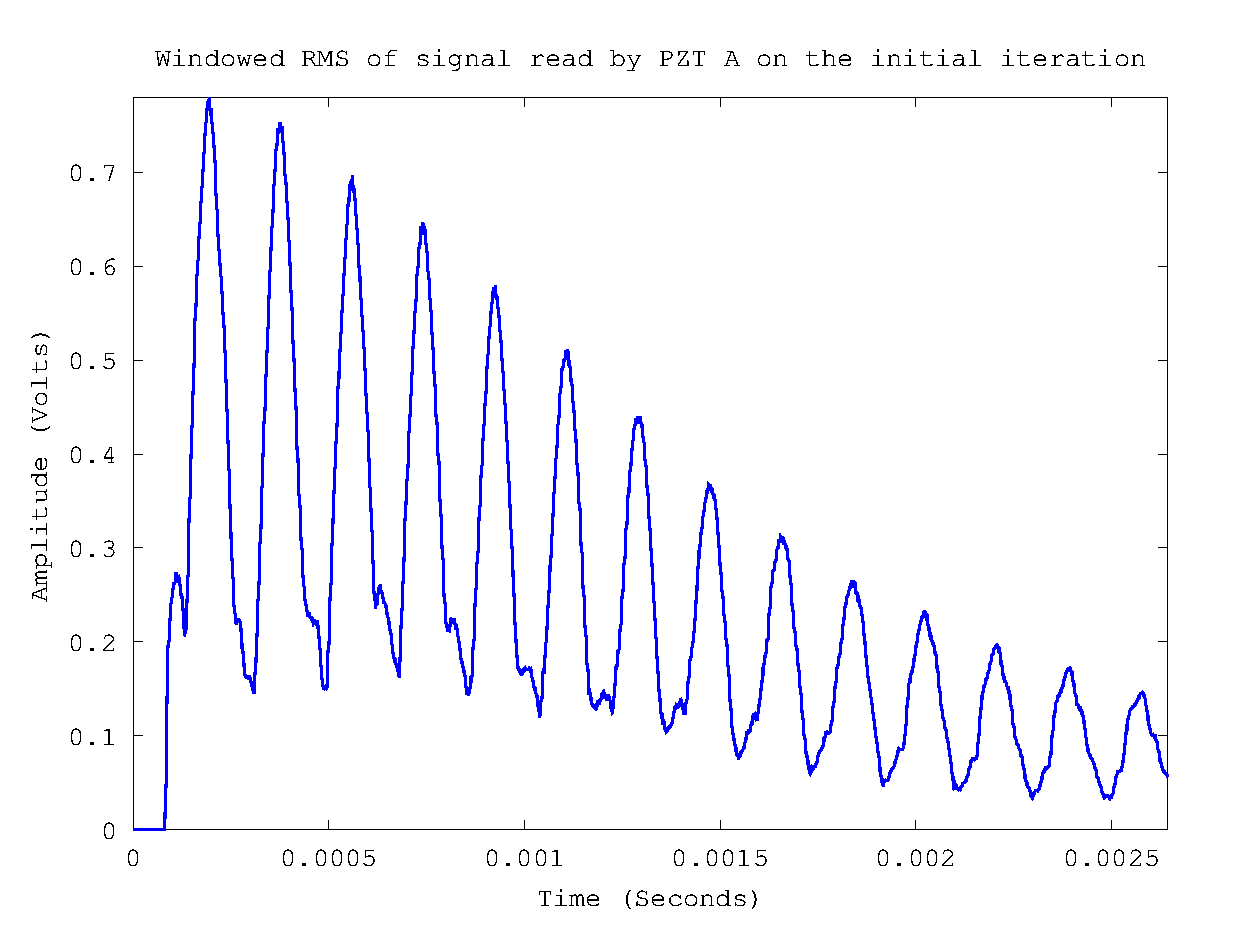
\includegraphics[width=9.7cm,height=5.75cm]{ch0RMS.eps}}
\subfigure[PZT B Windowed RMS]
{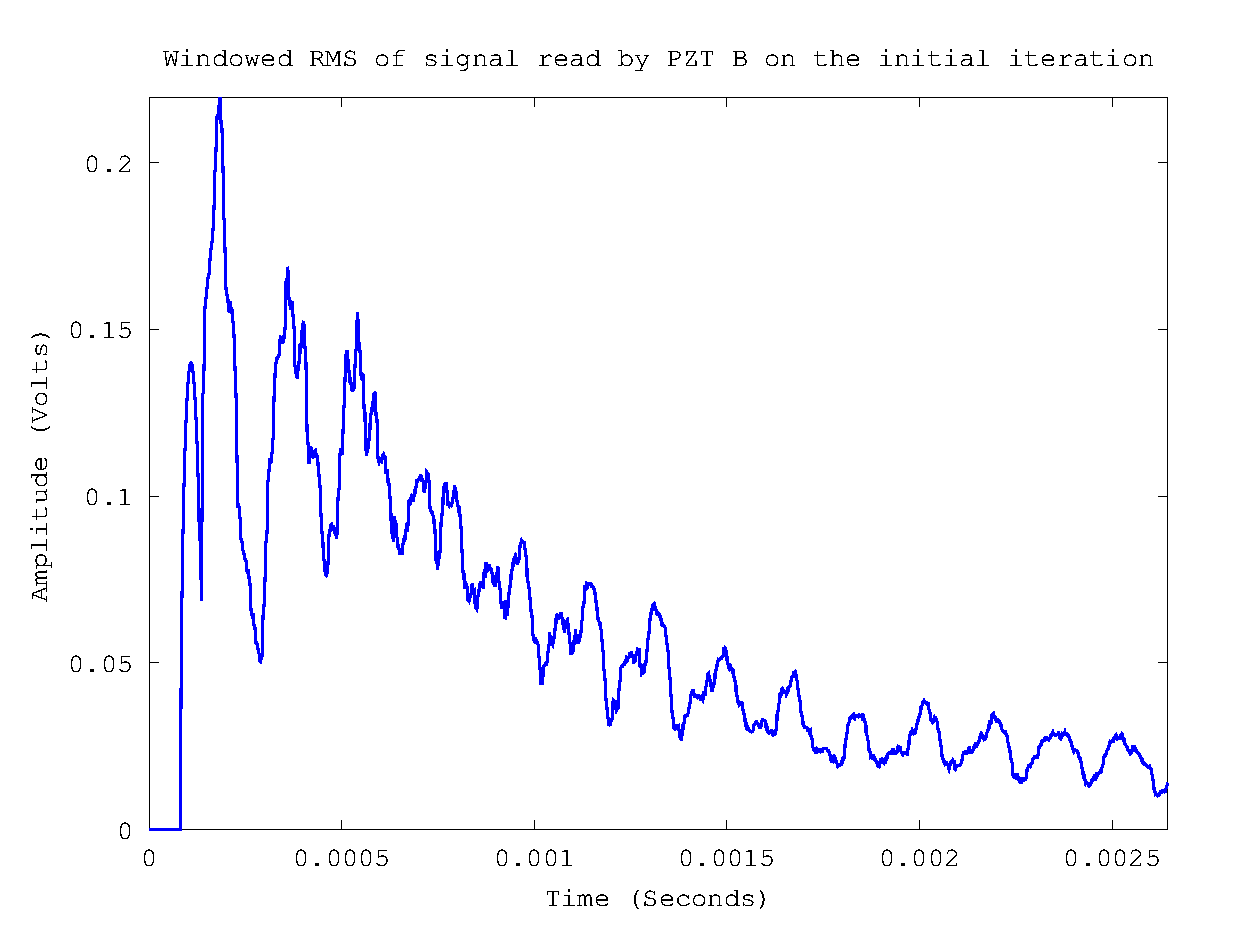
\includegraphics[width=9.7cm,height=5.75cm]{ch1RMS.eps}}
\end{subfigmatrix}

   \caption[all]
%>>>> use \label inside caption to get Fig. number with \ref{}
   { \label{windowedRMS}
(a) Windowed RMS (with a window length of 40 data points) of the signal read by PZT A for the $437$ mm and $428$ mm rods. The first 100 data points were zeroed out so that the internal PZT ringing from the wave that was played out did not overshadow the reflection waves. The largest peak was seen around the 144th data point. This data point marked the start of the window to that was extracted and played back by PZT A during the time reversal phase.;
(b) Windowed RMS of the signal read by PZT B. Here, the largest RMS peak occurred around the 136th data point which was where the extraction window began for the signal played back by PZT B during the time reversal phase.
 }
   \end{figure}

Once the location of the first wave occurrence was determined for PZT A, a window was extracted from its (PZT A) recorded signal which started at the time location of the RMS peak. The extraction length used was 60 data points and was based upon the original wave size of 40 points as to leave room for error in finding the wave location, but small enough to exclude vibrations which were not part of the original reflection wave (Figure \ref{selectedWindows}). This extracted window was then centered on zero, rescaled to be maximum amplitude, and then time reversed such that what was the last data point in the window became the first. (An identical procedure was used for the signal read by PZT B; determine the extraction location, extract the window, center, scale, and reverse  (Figure \ref{scaledWindows})).

\begin{figure}
\begin{subfigmatrix}{2}
\subfigure[PZT A Selected Window]
{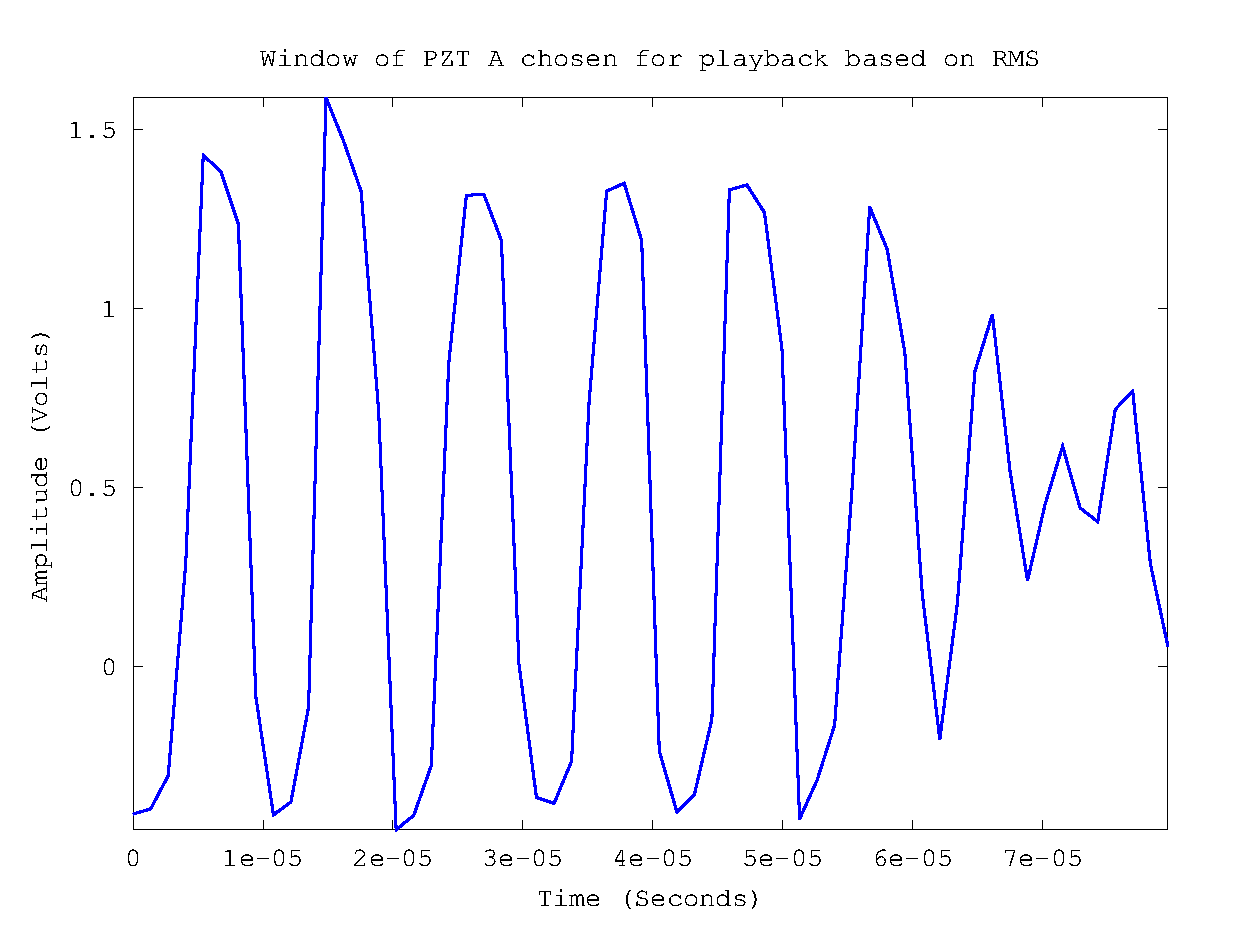
\includegraphics[width=9.7cm,height=5.75cm]{ch0Chosen.eps}}
\subfigure[PZT B Selected Window]
{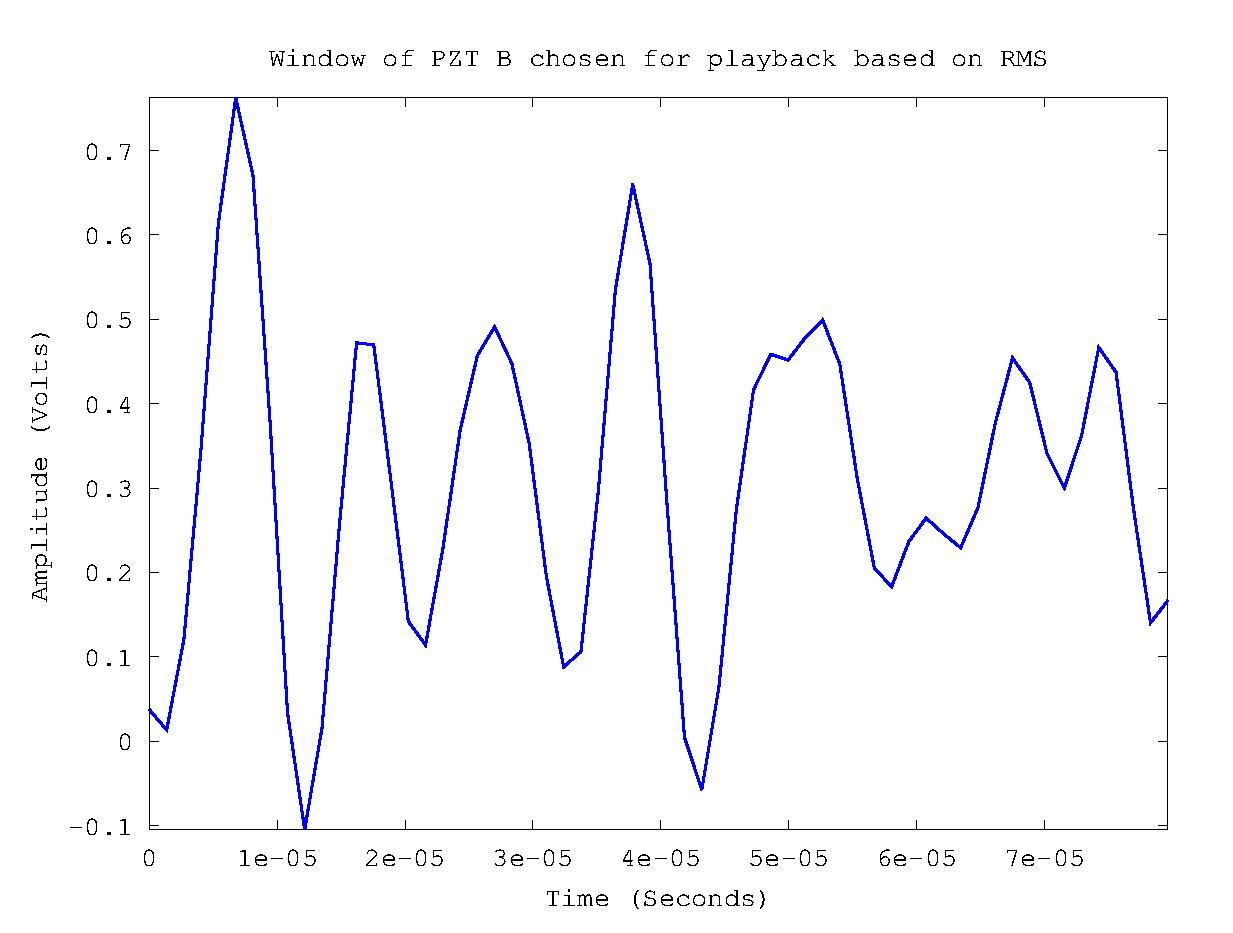
\includegraphics[width=9.7cm,height=5.75cm]{ch1Chosen.eps}}
\end{subfigmatrix}

   \caption[all]
%>>>> use \label inside caption to get Fig. number with \ref{}
   { \label{selectedWindows}
(a) Window of the signal read by PZT A that was selected for playback. This selection was based upon the maximum peak found in the windowed RMS graph of the signal read by PZT A;
(b) Window of the signal read by PZT B that was selected for playback. The selection process was the same as that for PZT A.
 }
   \end{figure}
   
 \begin{figure}
\begin{subfigmatrix}{2}
\subfigure[PZT A Centered, Scaled, Reversed Window]
{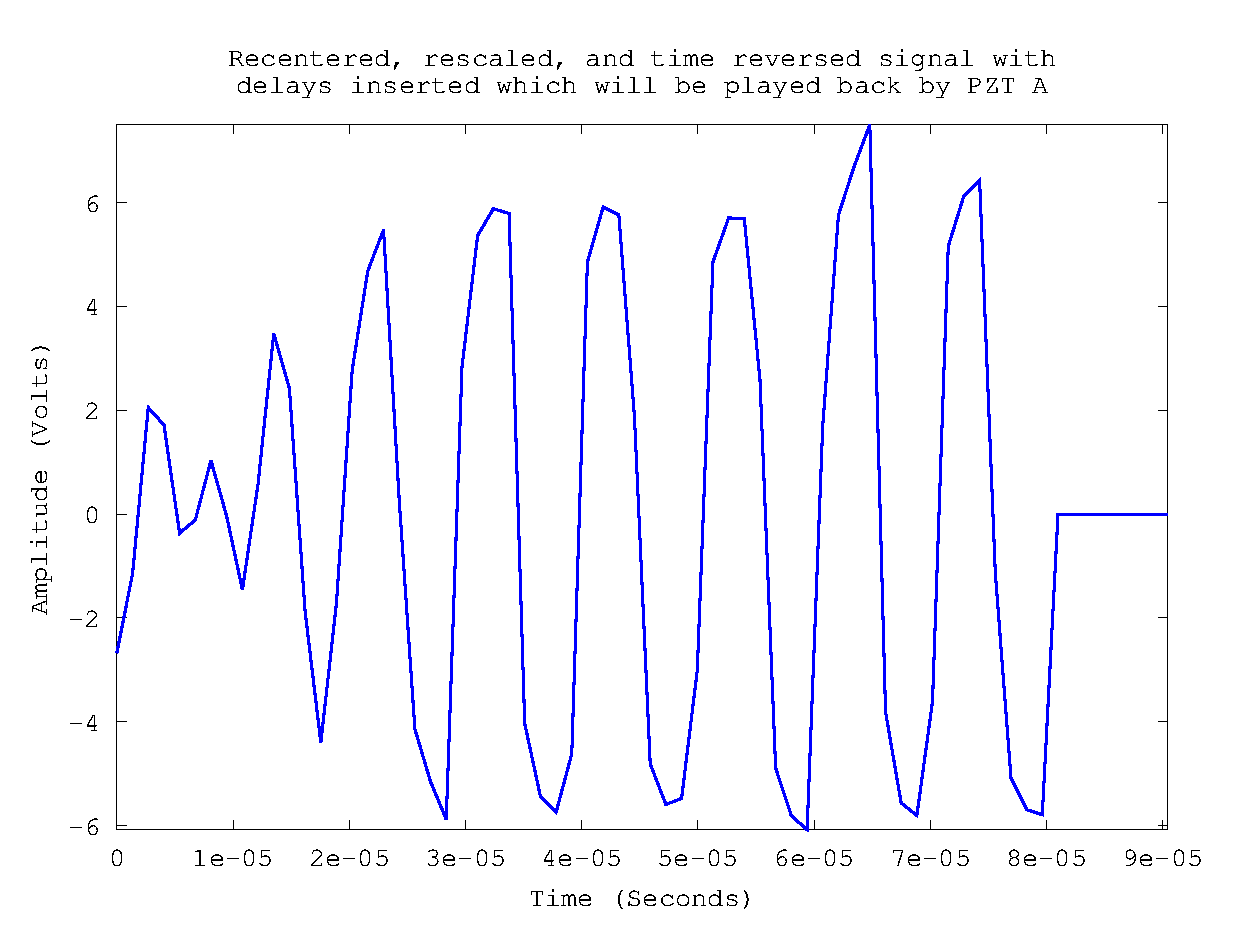
\includegraphics[width=9.7cm,height=5.75cm]{ch0Scaled.eps}}
\subfigure[PZT B Centered, Scaled, Reversed Window]
{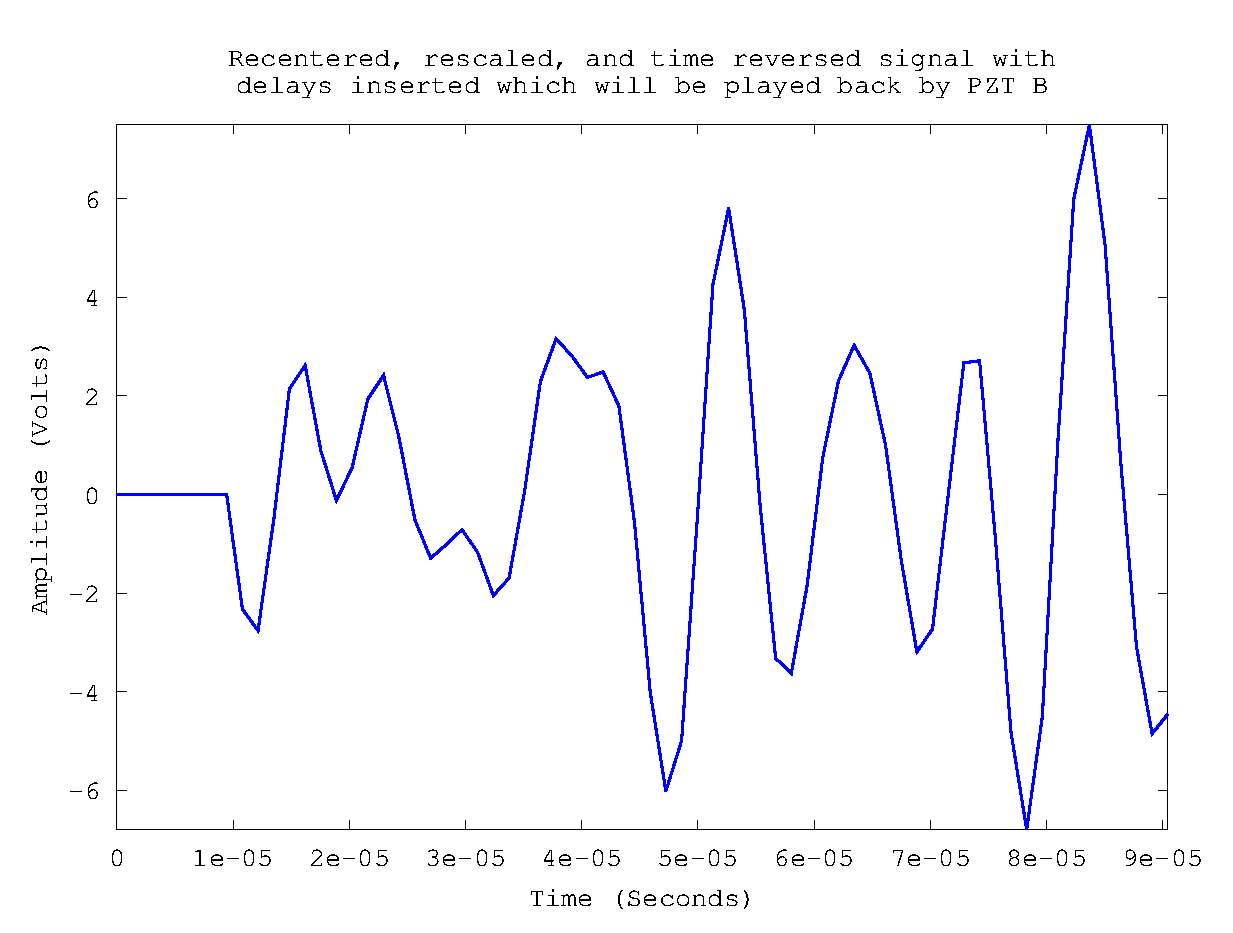
\includegraphics[width=9.7cm,height=5.75cm]{ch1Scaled.eps}}
\end{subfigmatrix}

   \caption[all]
%>>>> use \label inside caption to get Fig. number with \ref{}
   { \label{scaledWindows}
(a) Window that was played back by PZT A. It was centered on zero, scaled to be maximum amplitude, and time reversed such that last data point became the first.;
(b) Window that was played back by PZT B. It was also centered, scaled, and reversed. A delay was inserted at the beginning of PZT B. This is due to the fact that its wave window occurred sooner which means it is closer to the defect PZT. This delay was the difference between the time PZT B's wave was received and the time that PZT A's wave was received. This delay caused the waves to reach the defect at the same moment during the time reversal phase.
 }
   \end{figure}

After the windows were selected for playback, it was determined which PZT's window occurred first as it was assumed there was no prior knowledge of the actual rod lengths used. This step was important because the proper delays had to be inserted into the signals that were played back by each PZT in order for the signals to reach the defect at the same instant. In this sample test, it was found that PZT B had the first wave occurrence at data point 136; PZT A's wave occurrence was at 144 as mentioned in the caption for Figure \ref{windowedRMS}. The fill time in the time reversal window was the difference between occurrence time of the two channels (i.e., $ 144 - 136 = 8$) and was inserted at the start of the signal that was played back by PZT B. To keep the lengths consistent of the signals being played back, an equal fill time (8 points here) was inserted at the end of the signal that was played back by PZT A (Figure \ref{scaledWindows}).

Before playback, the software recorded the peak to peak amplitude of the response seen at the defect PZT for the current iteration so that it could be compared to future iterations. The signals were then sent back to the FPGA program from the host program. The FPGA waited the 200ms wait time that was specified to allow ringing in the rod to decay sufficiently. After this wait time, both PZT A and PZT B simultaneously played their time reversed signals. All three PZTs then also began recording as they did in the first iteration. The signals from each PZT propagated down the rod segments and reached the defect PZT at the same time. The waves met additively at the defect location which lead to a focusing of their energy at that point. The combined wave then split apart into multiple components that reflected back and forth between the PZTs. These reflections were recorded until the sample length was reached. Once the sample length was reached, the recorded data from each PZT was again transferred from the FPGA program to the host program. 

The entire time reversal and playback process was then repeated. However, this time the program no longer searched for the window that was needed to be reversed. For successive iterations, the information from the first iteration was used to extract a window from the recorded signal for PZT A and PZT B. These extracted windows were then centered on zero, scaled to maximum amplitude, and time reversed as above. The amplitude response seen at the defect was recorded. The processed windows were then played back by their respective PZTs. New information was recorded, and the process continued until the specified iteration number was reached (Figure \ref{flow}). The iteration number used in the tests was 150 as it was found that the played back signals did not change significantly by this point.

\begin{figure}
\begin{center}
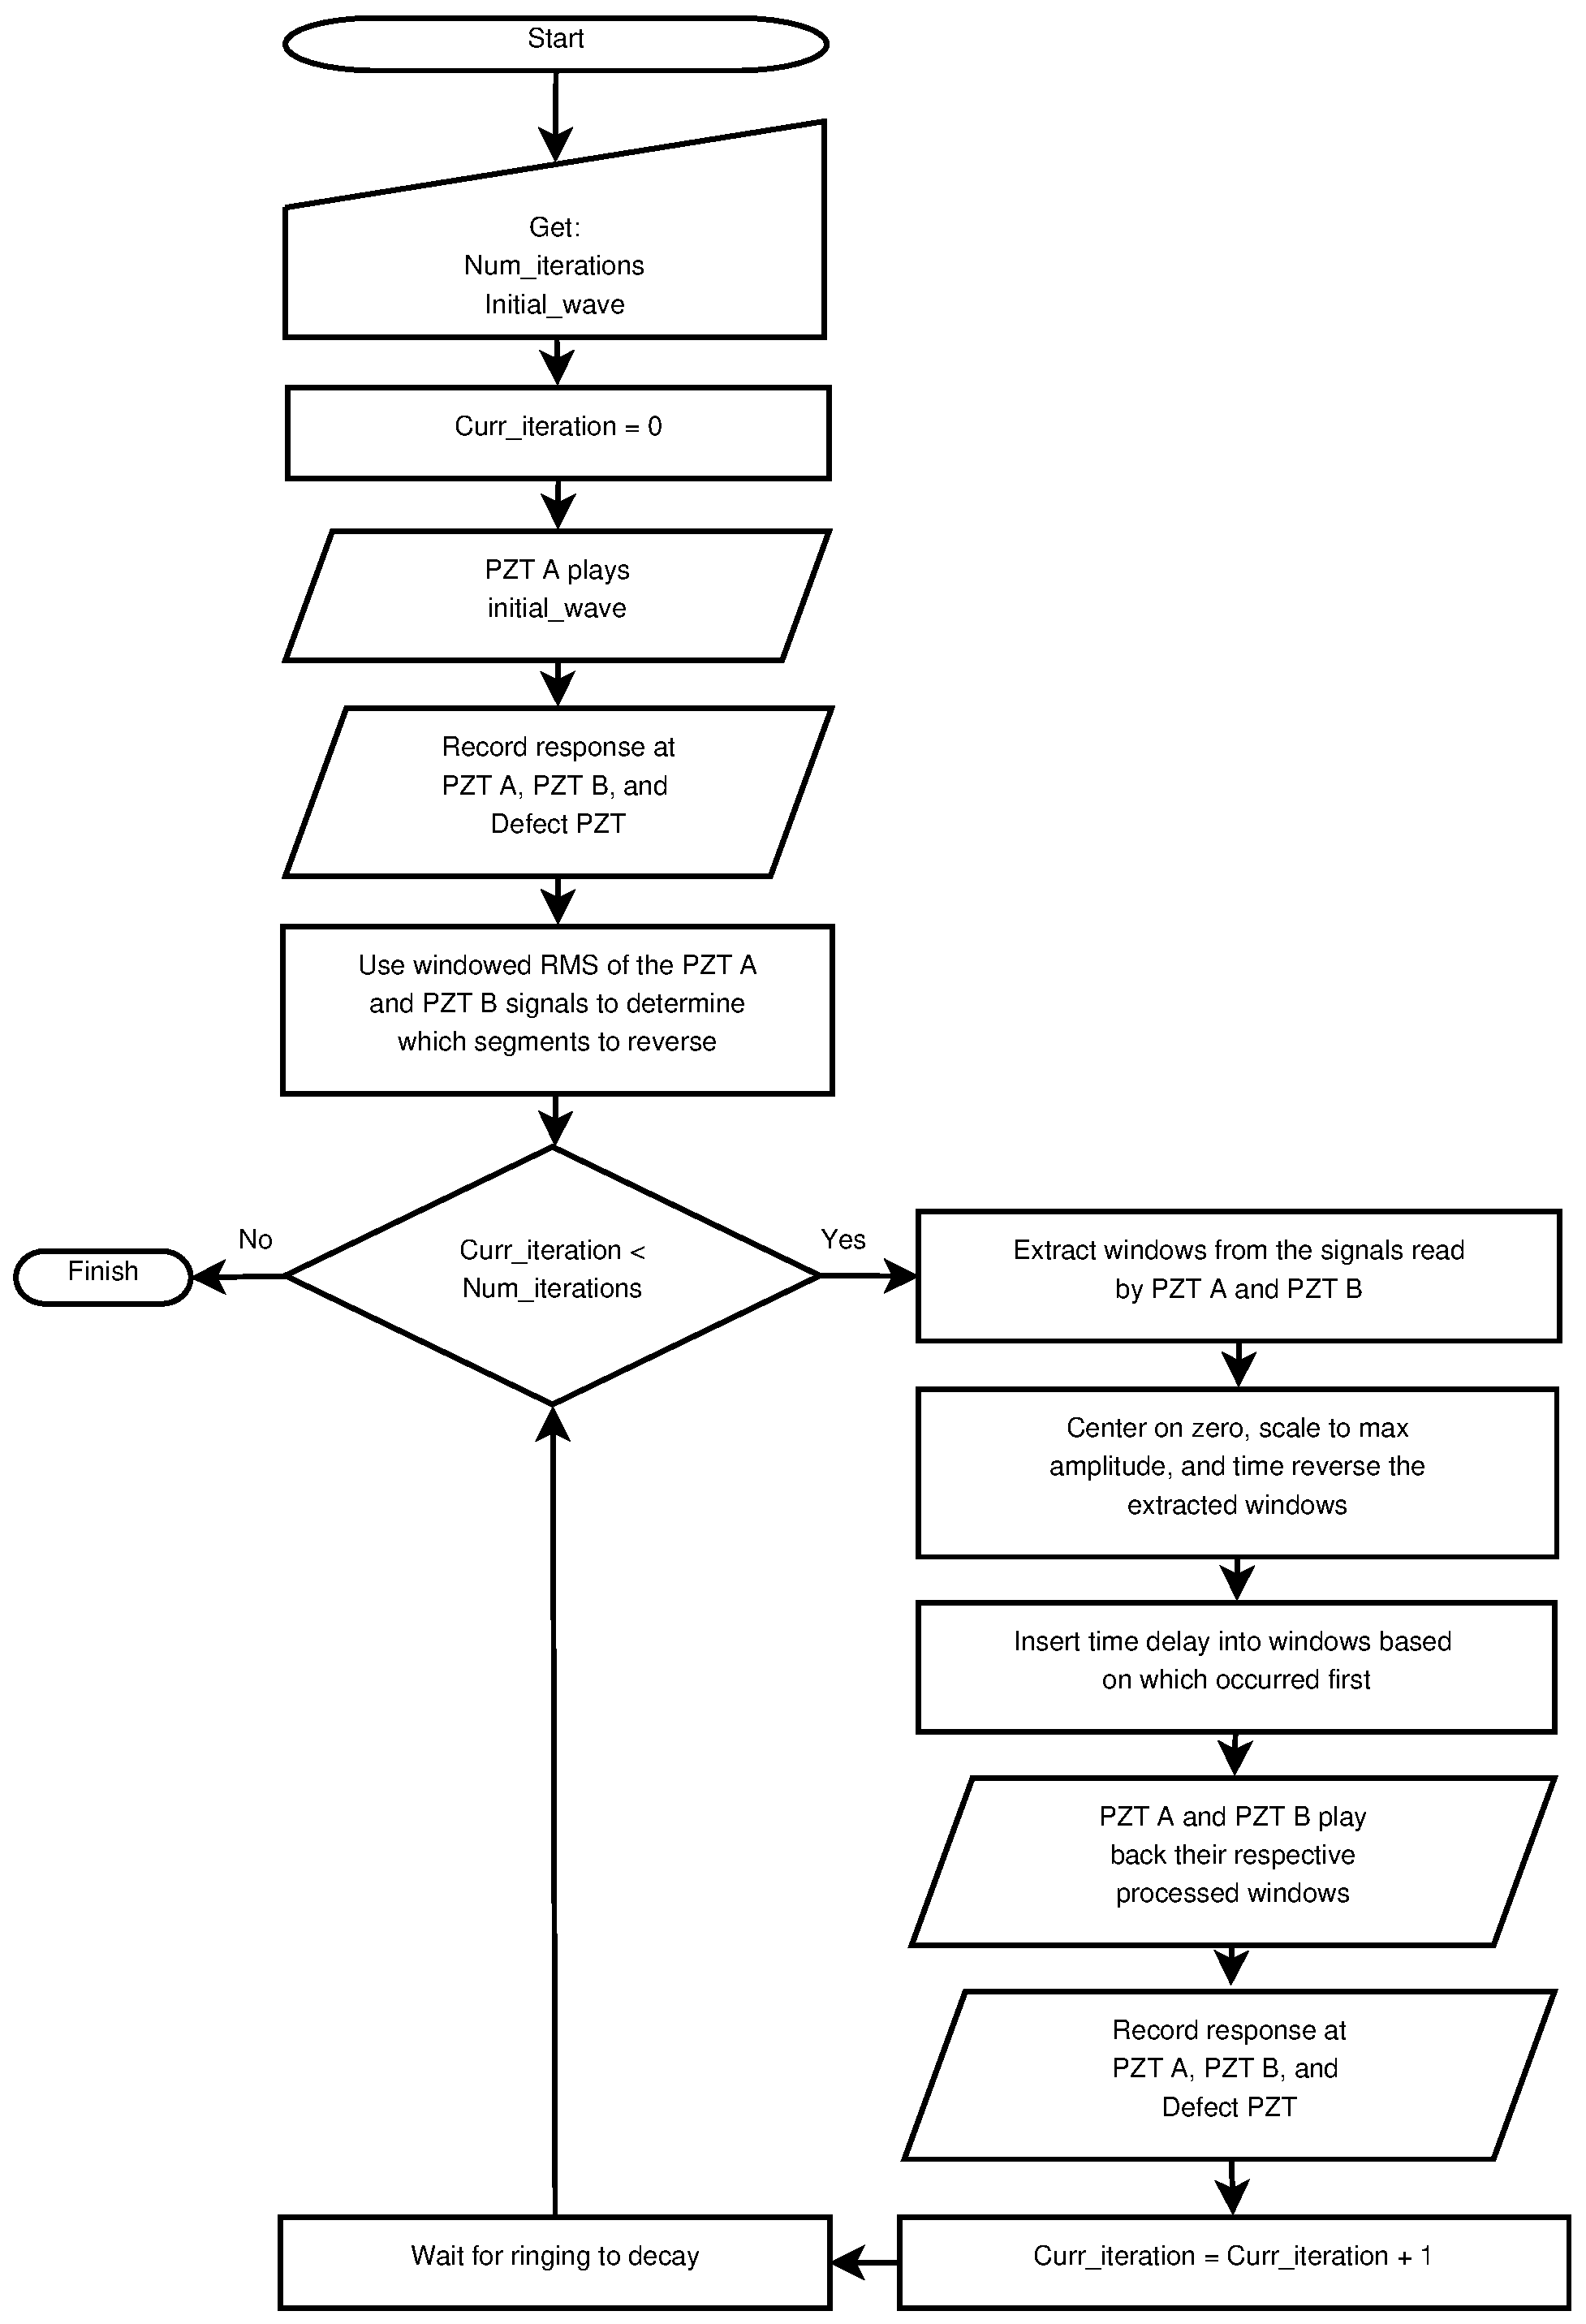
\includegraphics[width=15.7cm,height=15.75cm]{newFlow.eps}
\end{center}
% \vspace*{-20 pt}
 \caption[flo1]
%>>>> use \label inside caption to get Fig. number with \ref{}
   { \label{flow}
The logic-flow diagram summarizing the time reversal mirror
implementation.}
\end{figure}


\section{DISCUSSION OF RESULTS}
\label{sect:res}

The following section discusses the results obtained from the time reversal experiments that were previously described. These results were compared with the theoretical calculations. Six experiments in total were performed; three tests with steel rods and three tests with nylon rods.

\subsection{Steel Rod Results}
\label{sect:steelRodResults}

Figure \ref{steelThExp} depicts the theoretical results together
with the experimental results for time reversal mirror
action in a steel circular rod sample. As mentioned, time reversed focusing here
was sought at the `defect' transducer for a multi-tone
signal over frequencies 100-130 kHz. Calculations based
on equations (\ref{impdefect}) and (\ref{strconv2}) were carried
out assuming zero dissipation. Consistent with the absence of
dispersion, the signal was found to retain its shape through the
time reversal and play back processes.  While there appeared to be
a reasonable match between the predicted and measured results, the
present calculations ignore dissipation.  Also, the measurements
showed some alteration in the shape of the signal through the
process, indicating a small amount of dispersion in the
extensional-wave propagation even in the steel samples. 

 \begin{figure}
\begin{subfigmatrix}{3}
\subfigure[Theory vs Experiment, 579mm and 437mm steel rods]
{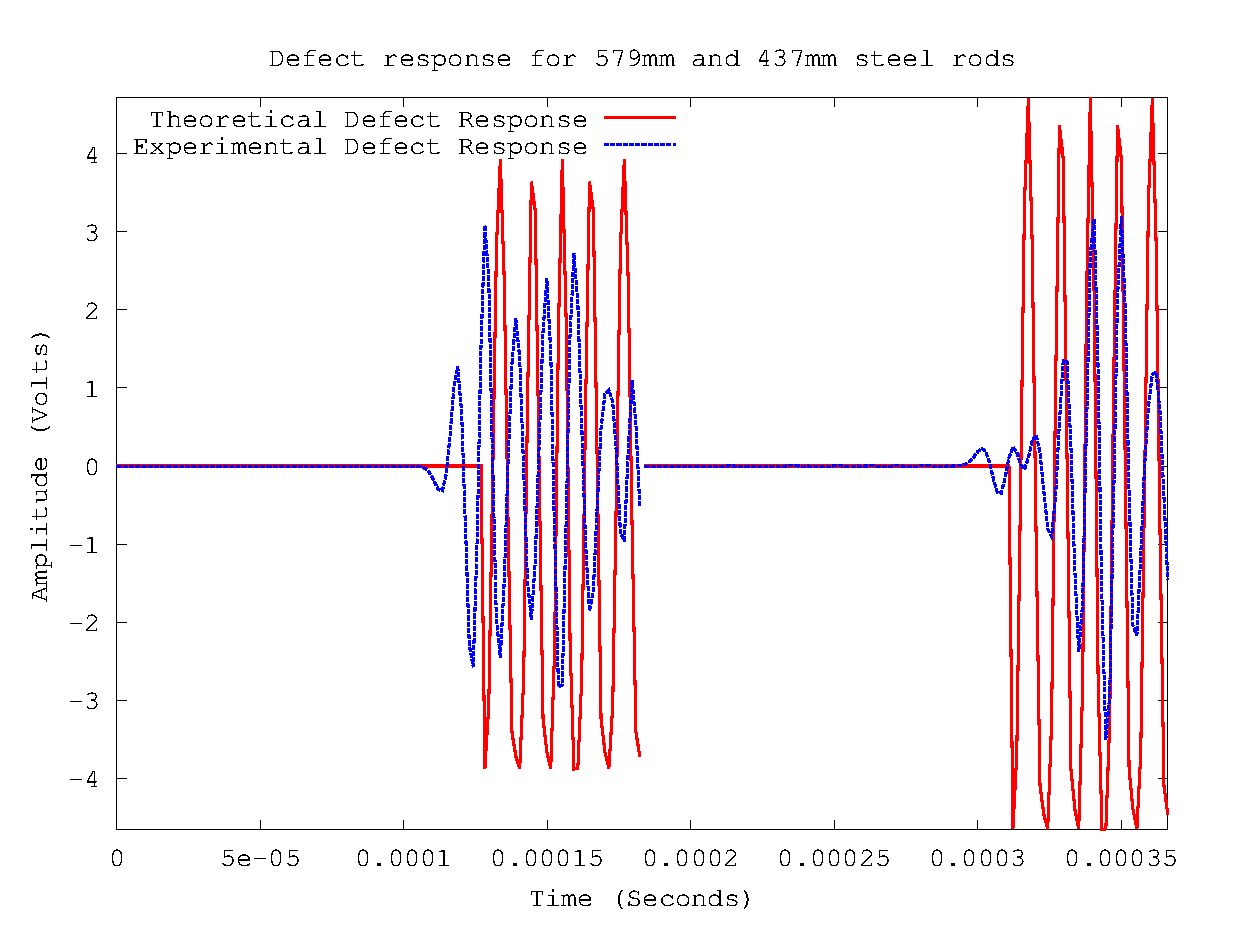
\includegraphics[width=9.7cm,height=5.75cm]{steel-1-2_Iter_th_exp.eps}}
\subfigure[Theory vs Experiment, 579mm and 428mm steel rods]
{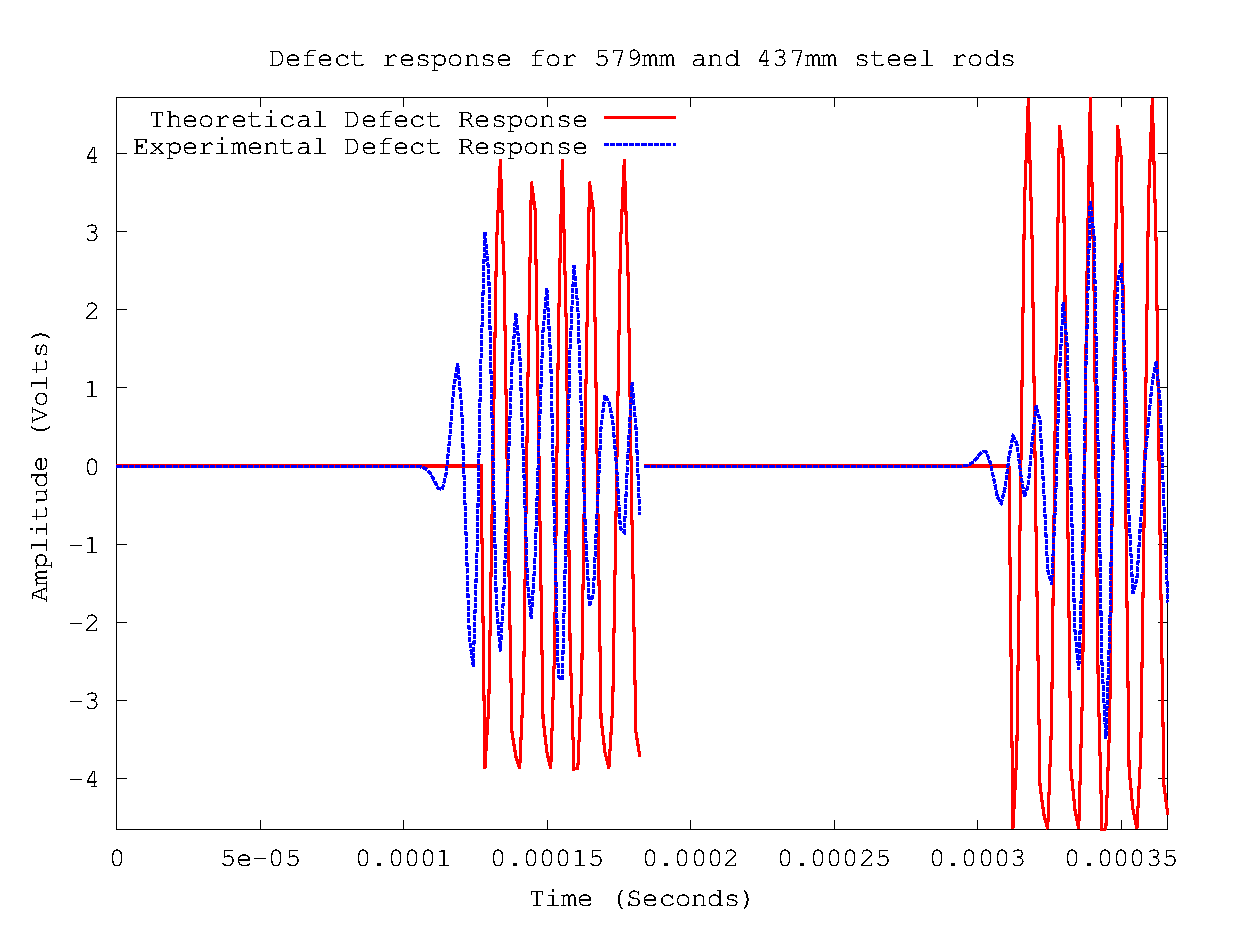
\includegraphics[width=9.7cm,height=5.75cm]{steel-1-3_Iter_th_exp.eps}}
\subfigure[Theory vs Experiment, 437mm and 428mm steel rods]
{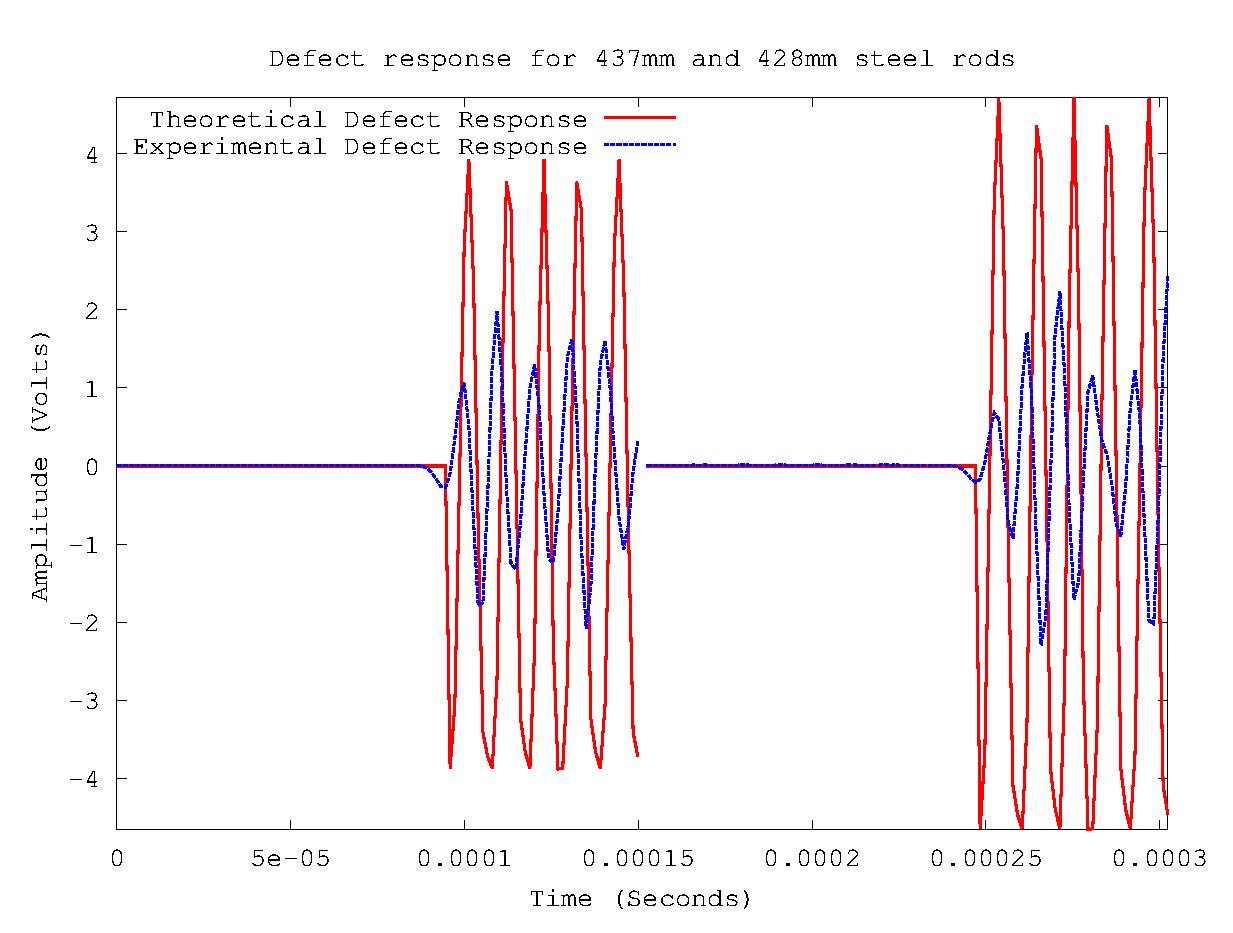
\includegraphics[width=9.7cm,height=5.75cm]{steel-2-3_Iter_th_exp.eps}}
\end{subfigmatrix}

   \caption[all]
%>>>> use \label inside caption to get Fig. number with \ref{}
   { \label{steelThExp}
Steel rod experimental results for the response seen at the defect PZT plotted with the theoretical calculations for the response. The results were plotted for each of the three steel rod tests. A reasonable match is seen vis-a-vis the wave phase and amplitude. The discrepancies could be explained by the calculations not accounting for effects from dispersion or dissipation.
 }
 \end{figure}

The goal of iteratively applying the time reversal algorithm was to increase the stress-wave induced response at the defect with each iteration. The amplitude gain that was achieved on each iteration at the defect PZT was used to determine the effectiveness of the present algorithm. To determine the gain, the maximum amplitude seen at the defect on each iteration was compared to the amplitude seen on the initial iteration. The maximum amplitude response was taken as $|max(defectVoltage) - min(defectVoltage)|$. The gain was calculated as $currentMax / initialMax$ and was plotted for each iteration of the time reversal algorithm. It was seen in the steel rod tests that the gain quickly increased in the beginning as the algorithm found a better quality signal to reverse for each PZT. As the number of iterations grew, the gain began to level off which implied a convergence of the replayed signals. The gain plots for each of the three steel rod tests showed that a considerable gain was reached within the first 25 iterations (Figures \ref{steelExp1} - \ref{steelExp3}). It was seen that the convergence gain may not be the maximum gain that was achieved throughout the iterative process. This suggests that further refinements could be made to the algorithm in order to achieve a more optimal solution, and further understanding of the phenomena is needed through more penetrative modeling.

Another good measure of the effectiveness of the iterative time reversal process was to compare the wave seen at the defect on the first iteration to the wave seen on the last iteration. What should have been observed is that the wave on the final iteration was a much more defined (i.e., purer) form of the initial wave. This final wave ideally would have an amplitude larger than the wave amplitude that was initially recorded. For the steel rod tests this exact behavior was observed . Figures \ref{steelExp1}-\ref{steelExp3} show a side-by-side comparison of the initial wave at the defect PZT and the final wave at the defect PZT. Graphs were produced for each steel rod test and each showed a large improvement in wave amplitude/quality as a result of the iterative time reversal algorithm.

 \begin{figure}
\begin{subfigmatrix}{3}
\subfigure[Defect Response Initial Iteration, 579mm and 437mm steel rods]
{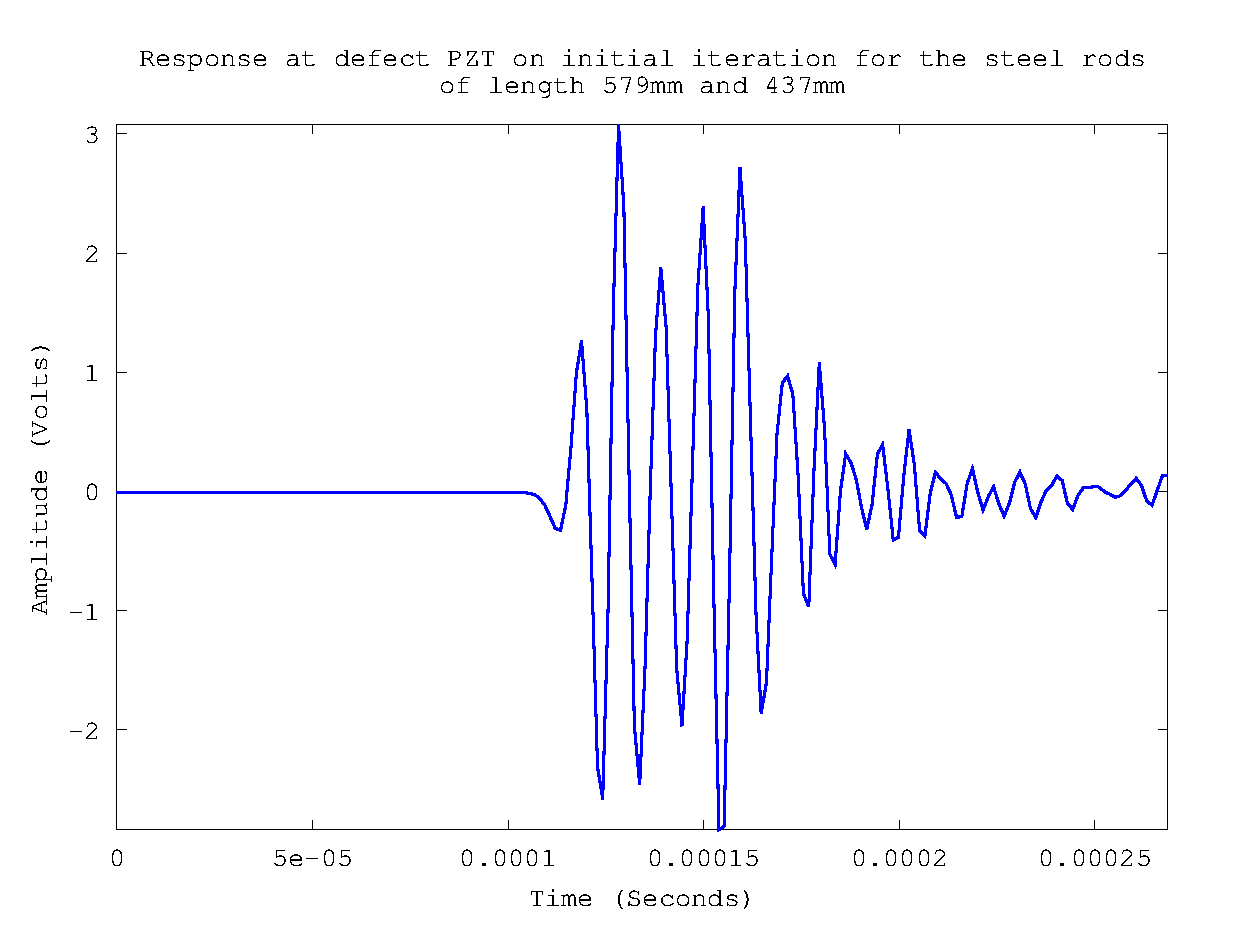
\includegraphics[width=9.7cm,height=5.75cm]{steel-1-2_Initial.eps}}
\subfigure[Defect Response 150th Iteration, 579mm and 437mm steel rods]
{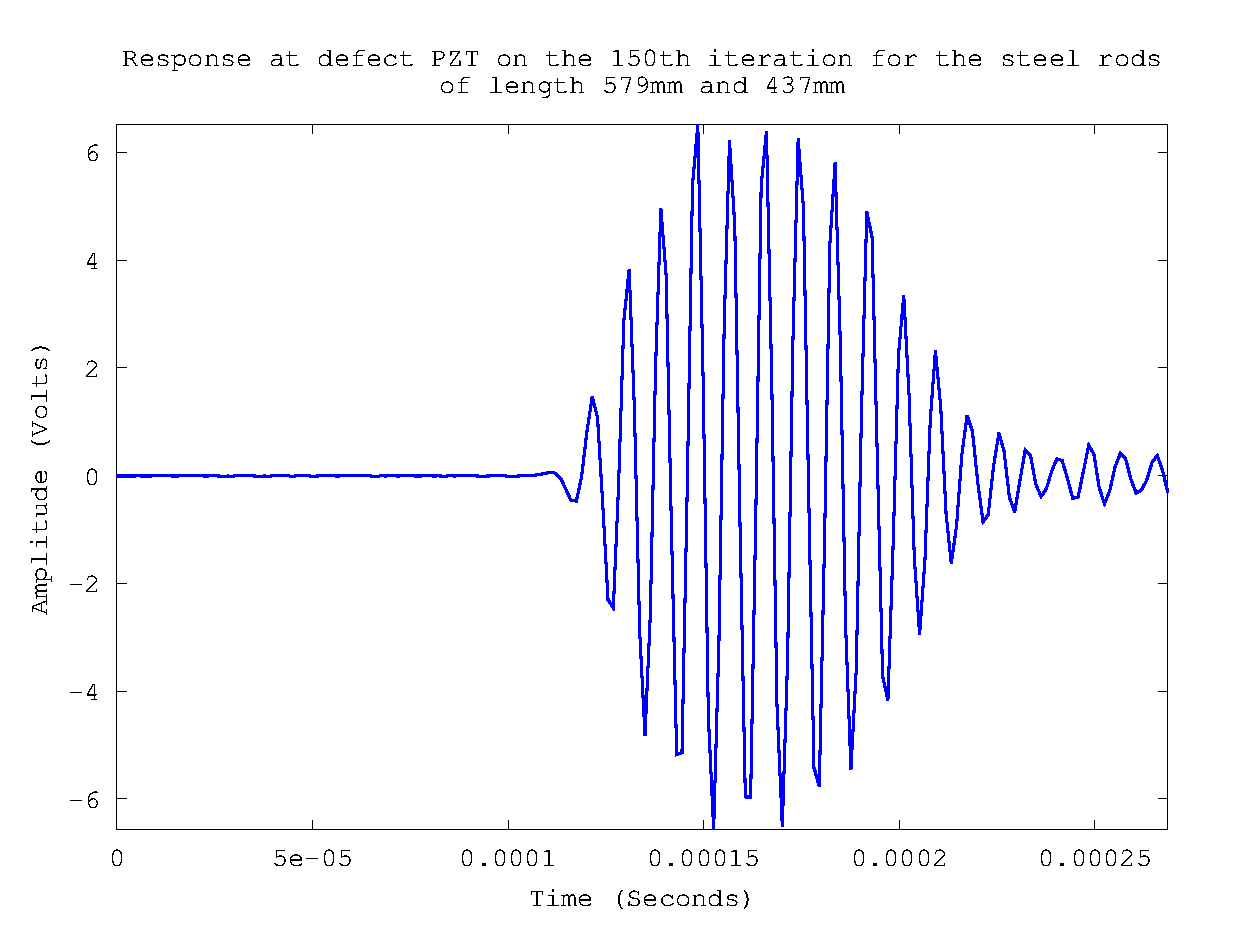
\includegraphics[width=9.7cm,height=5.75cm]{steel-1-2_Final.eps}}
\subfigure[Defect Amplitude Gain, 579mm and 437mm steel rods]
{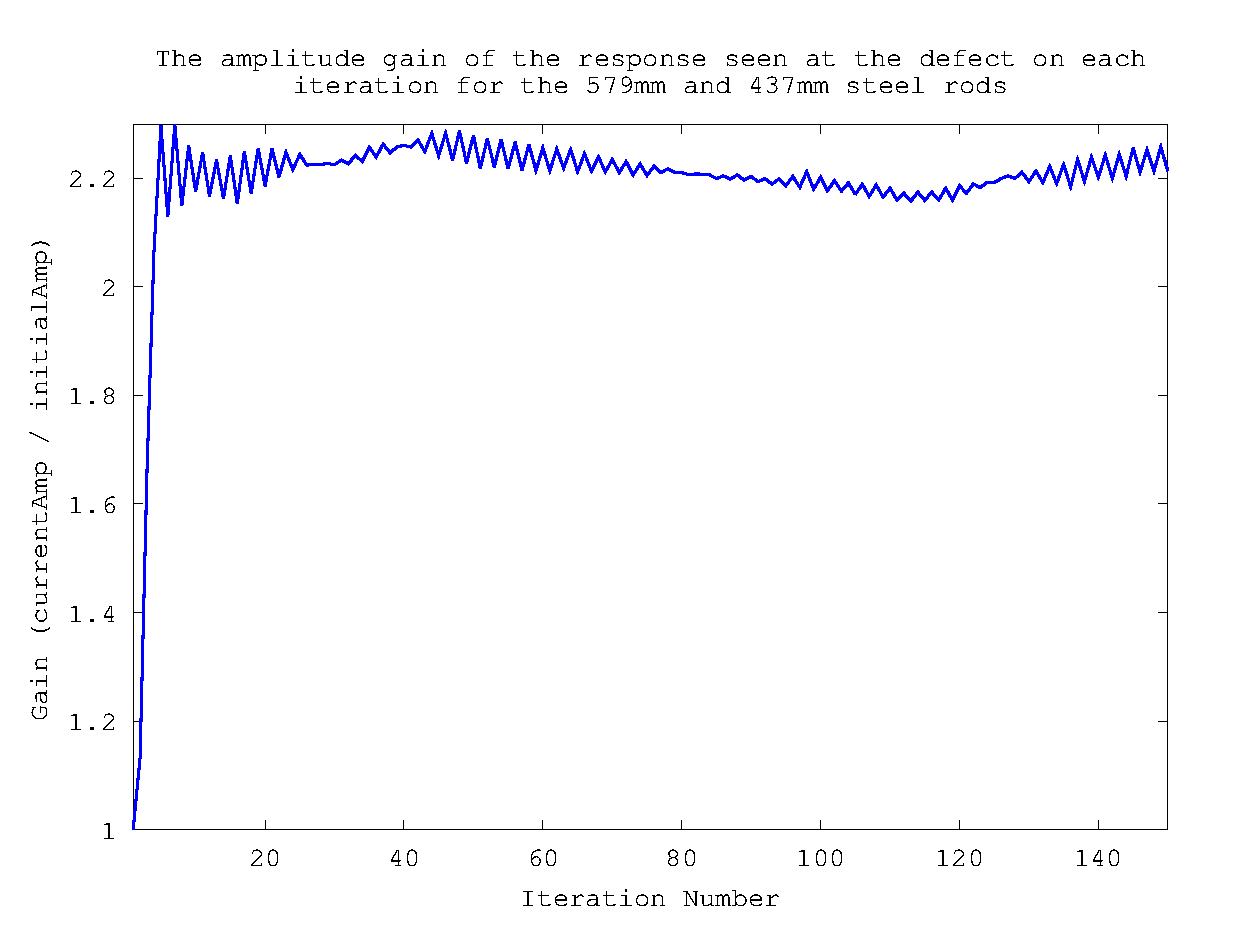
\includegraphics[width=9.7cm,height=5.75cm]{steel-1-2_iterationVsGain.eps}}
\end{subfigmatrix}

   \caption[all]
%>>>> use \label inside caption to get Fig. number with \ref{}
   { \label{steelExp1}
   a) First wave seen at the defect on the initial iteration for the 579mm and 437mm steel rod test.; b) Wave recorded at the defect after 150 iterations. The wave was much more defined and more than doubled in amplitude since the first iteration.; c) Plot of the amplitude gain that was achieved at the defect for each iteration of the time reversal algorithm, with a convergence gain of a little over 2. The gain did not appear to completely level out, but it slowly oscillated right around 2.
 }
\end{figure}

 \begin{figure}
\begin{subfigmatrix}{3}
\subfigure[Defect Response Initial Iteration, 579mm and 428mm steel rods]
{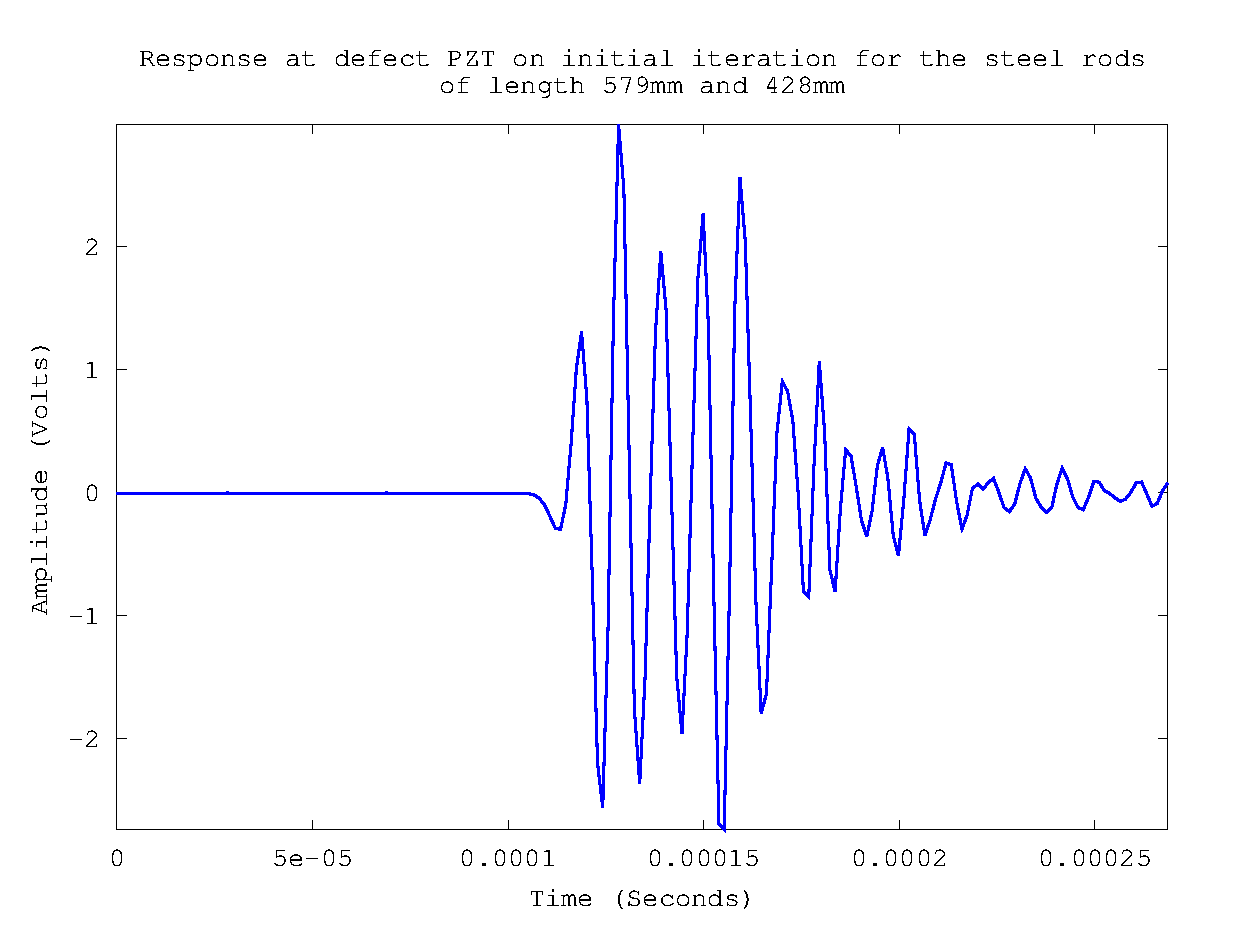
\includegraphics[width=9.7cm,height=5.75cm]{steel-1-3_Initial.eps}}
\subfigure[Defect Response 150th Iteration, 579mm and 428mm steel rods]
{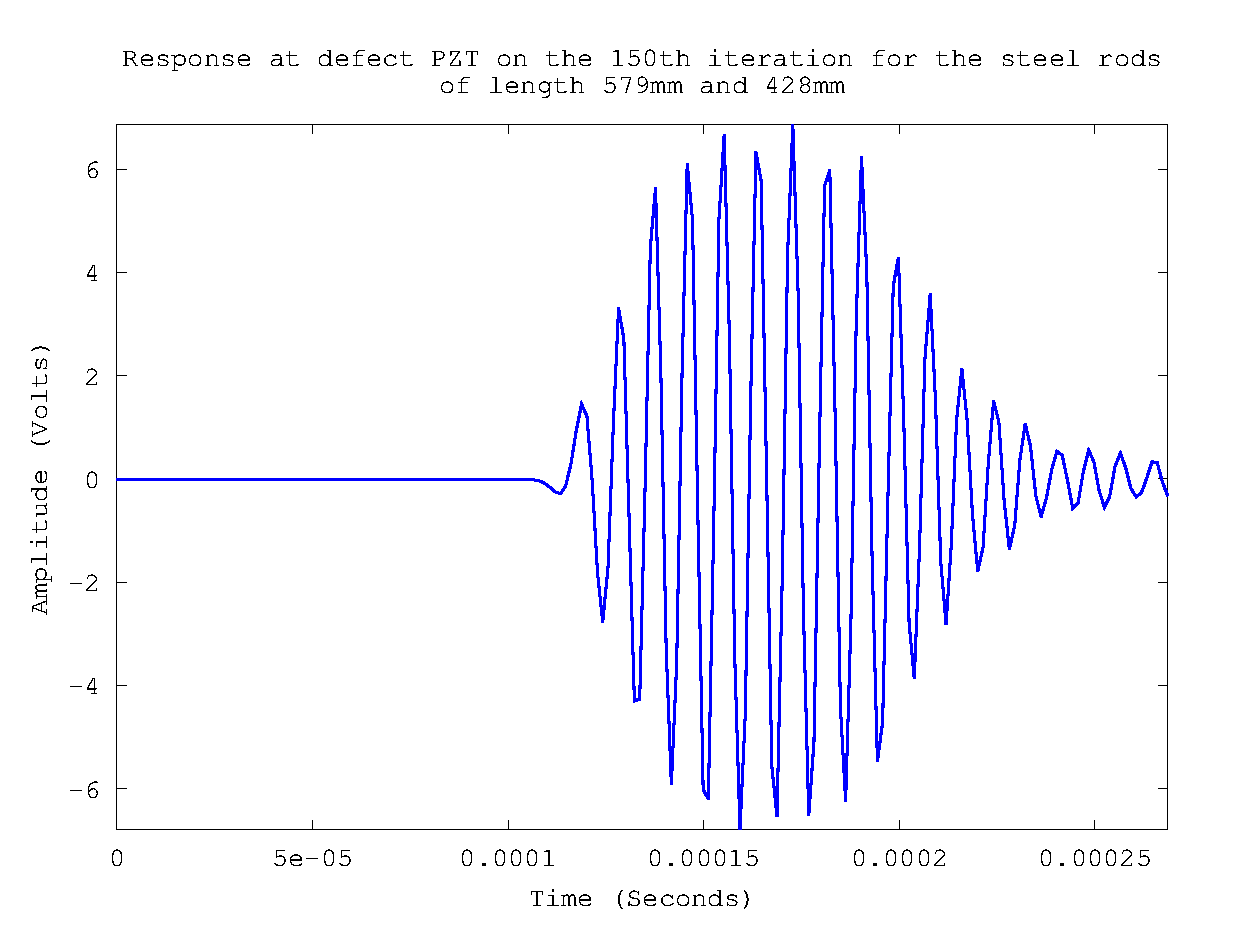
\includegraphics[width=9.7cm,height=5.75cm]{steel-1-3_Final.eps}}
\subfigure[Defect Amplitude Gain, 579mm and 428mm steel rods]
{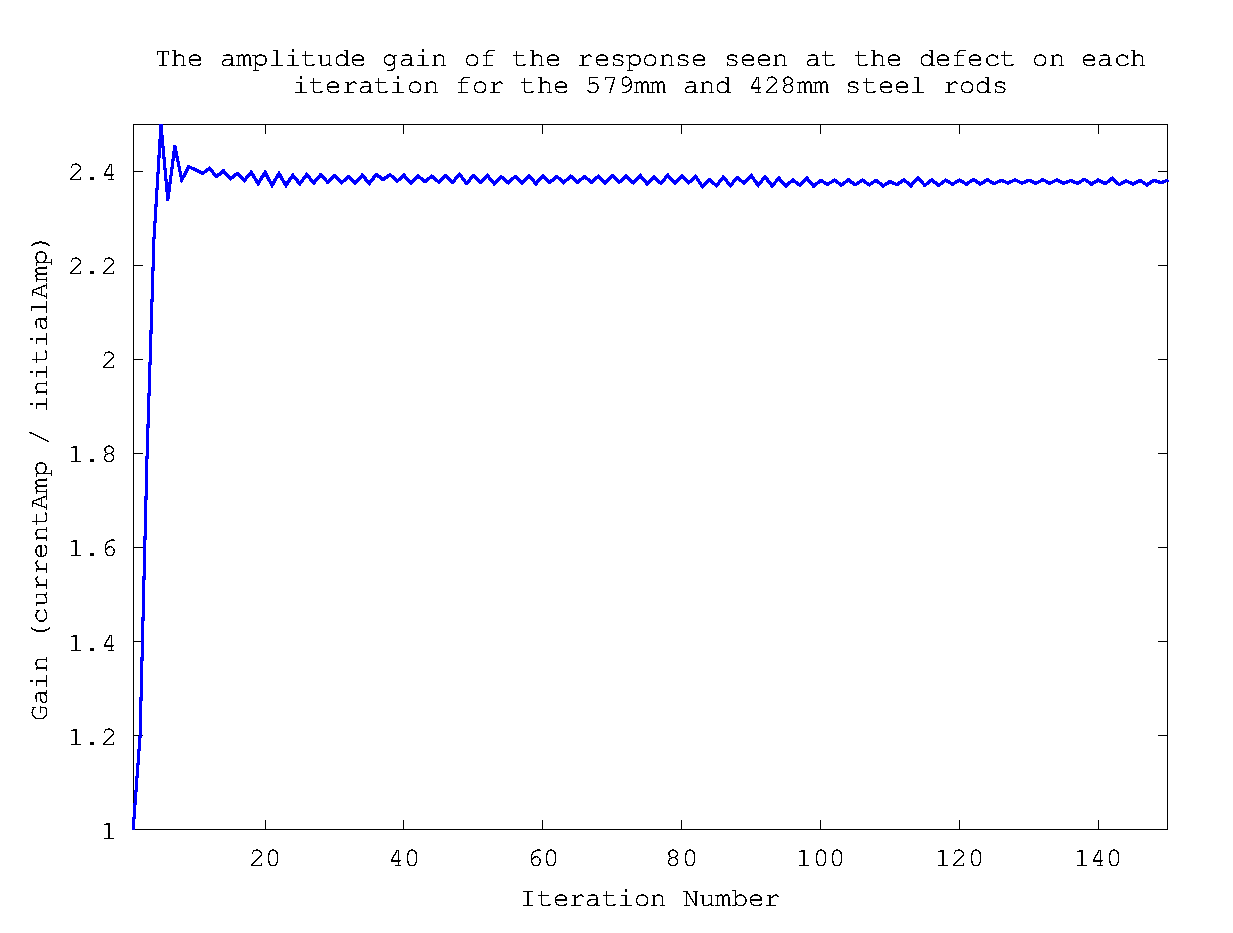
\includegraphics[width=9.7cm,height=5.75cm]{steel-1-3_iterationVsGain.eps}}
\end{subfigmatrix}

   \caption[all]
%>>>> use \label inside caption to get Fig. number with \ref{}
   { \label{steelExp2}
   a) First wave seen at the defect on the initial iteration for the 579mm and 428mm steel rod test.; b) Wave recorded at the defect after 150 iterations. Like the 579mm and 437mm steel rod results, this wave was much more defined and more than doubled in amplitude since the first iteration.; c) Plot of the amplitude gain that was achieved at the defect for each iteration of the time reversal algorithm, with a convergence gain of about 2.5.
 }
\end{figure}

 \begin{figure}
\begin{subfigmatrix}{3}
\subfigure[Defect Response Initial Iteration, 437mm and 428mm steel rods]
{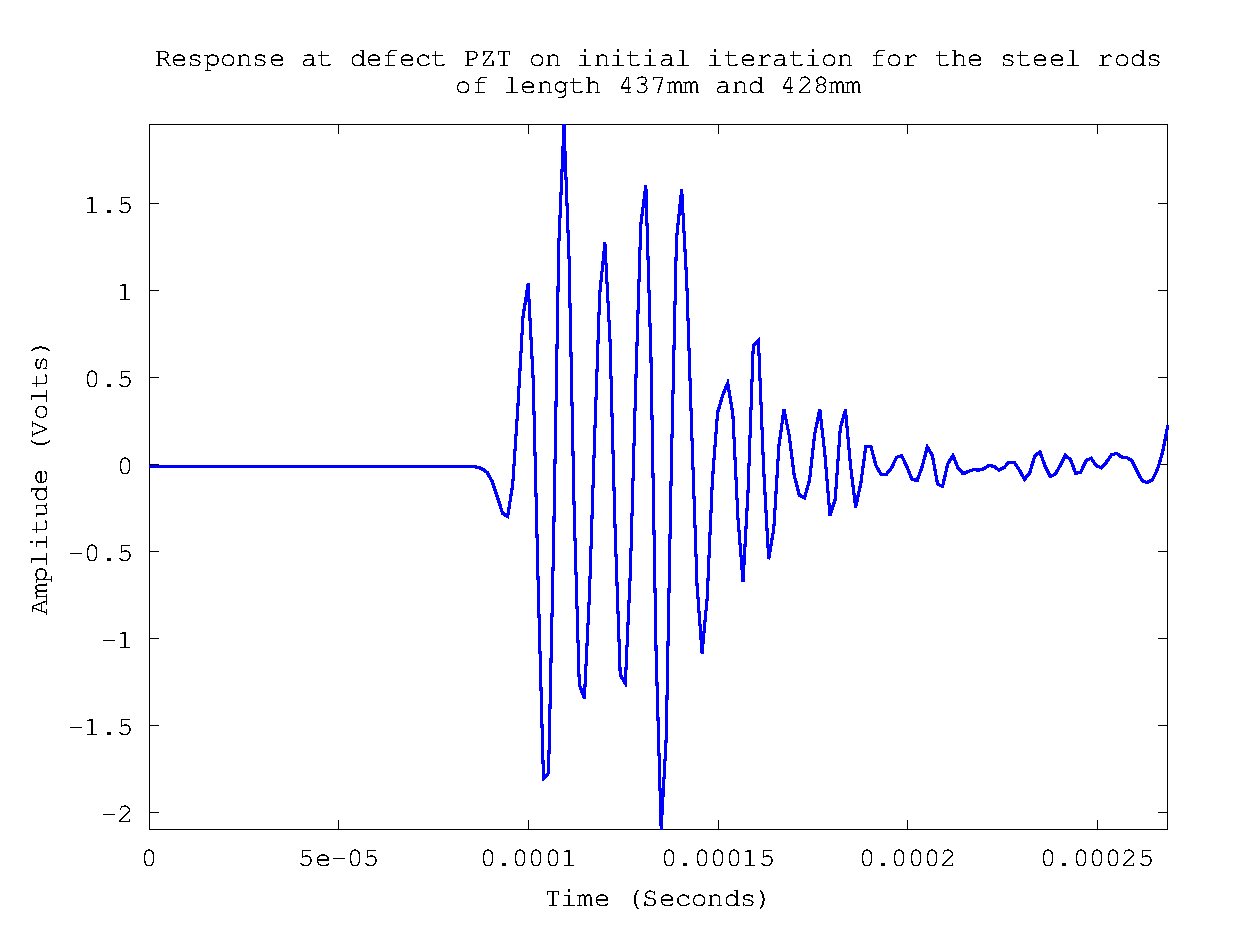
\includegraphics[width=9.7cm,height=5.75cm]{steel-2-3_Initial.eps}}
\subfigure[Defect Response 150th Iteration, 437mm and 428mm steel rods]
{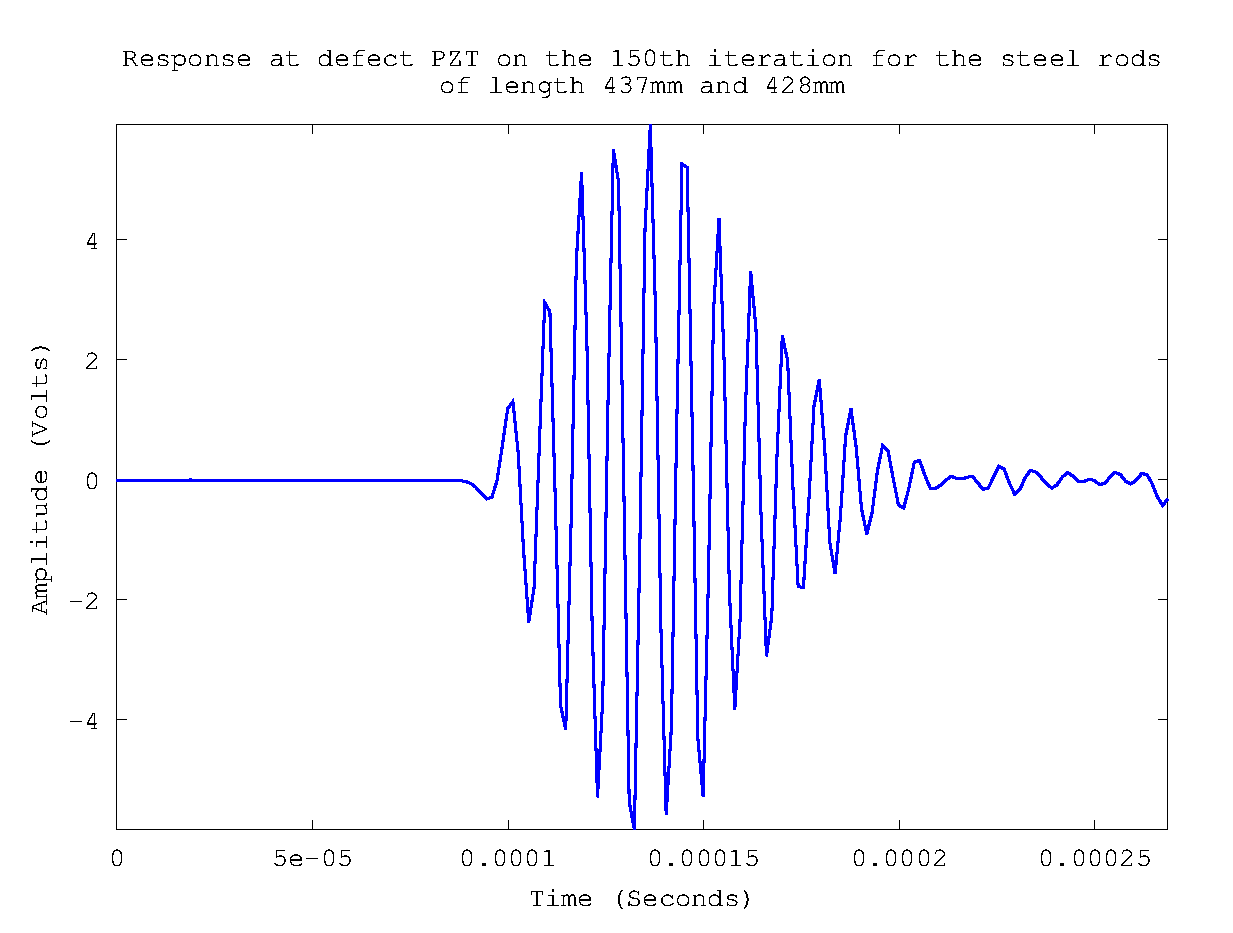
\includegraphics[width=9.7cm,height=5.75cm]{steel-2-3_Final.eps}}
\subfigure[Defect Amplitude Gain, 437mm and 428mm steel rods]
{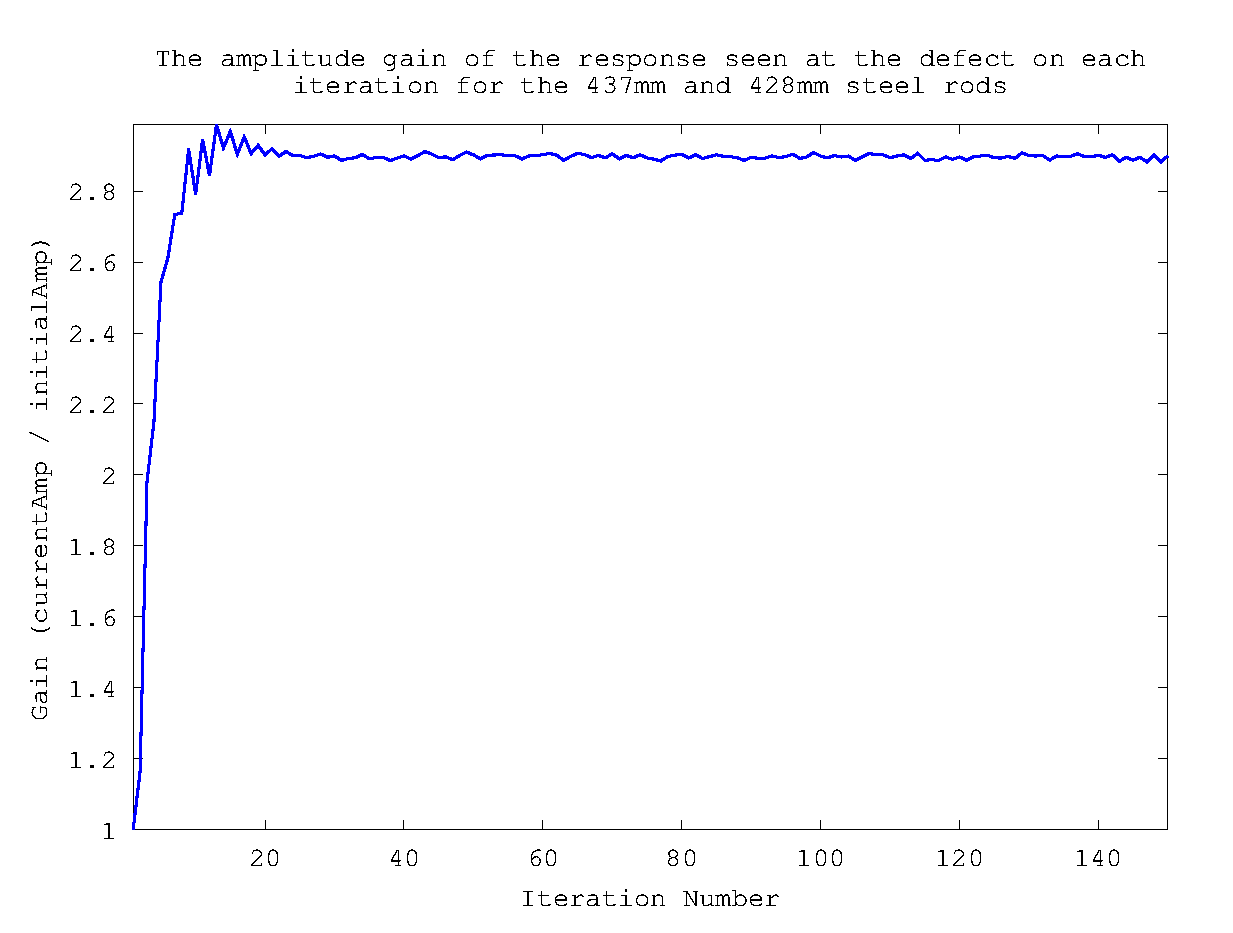
\includegraphics[width=9.7cm,height=5.75cm]{steel-2-3_iterationVsGain.eps}}
\end{subfigmatrix}

   \caption[all]
%>>>> use \label inside caption to get Fig. number with \ref{}
   { \label{steelExp3}
   a) First wave seen at the defect on the initial iteration for the 437mm and 428mm steel rod test.; b) Wave recorded at the defect after 150 iterations. The amplitude of the wave nearly tripled since the first iteration; c) Plot of the amplitude gain that was achieved at the defect for each iteration of the time reversal algorithm, with a convergence gain of about 3.
 }
\end{figure}

\subsection{Nylon Rod Results}
\label{sect:nylonRodResults}

As with the steel rods, calculations were carried out for the nylon rods based upon the theory laid out in the beginning of this paper. These theoretical results were compared to the results obtained from real life experiments with the nylon rods. Dissipation and dispersion were also ignored in these calculations. Figure \ref{nylonThExp} shows the theoretical and experimental results for the nylon rods. A worse match was seen between the expected and actual responses, perhaps due to the greater dispersion and dissipation than in the steel rods. For each experiment, however, it was still observed that the amplitude of the second wave was larger than that of the first.

 \begin{figure}
\begin{subfigmatrix}{3}
\subfigure[Theory vs Experiment, 148mm and 105mm nylon rods]
{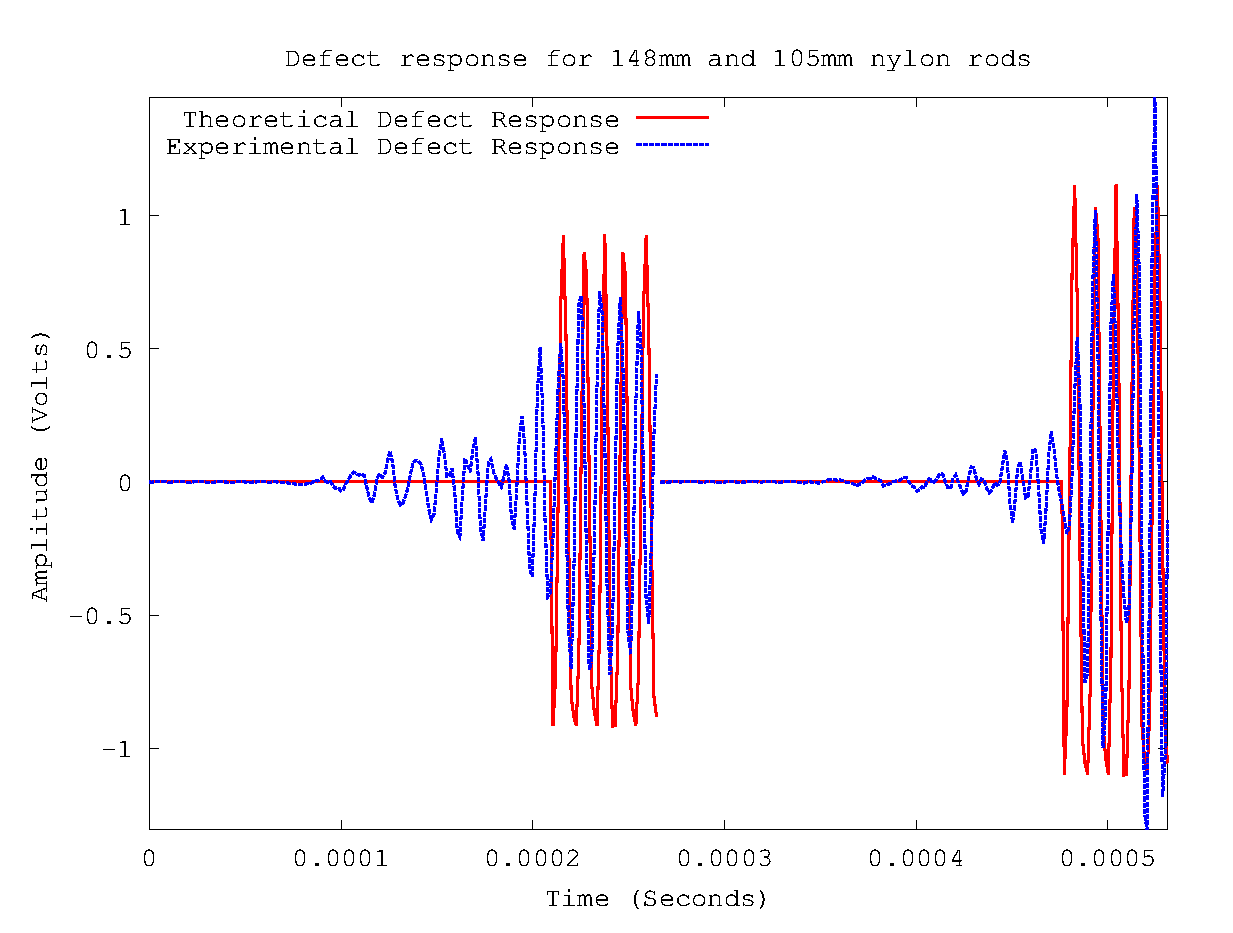
\includegraphics[width=9.7cm,height=5.75cm]{nylon-2-3_Iter_th_exp.eps}}
\subfigure[Theory vs Experiment, 148mm and 75mm nylon rods]
{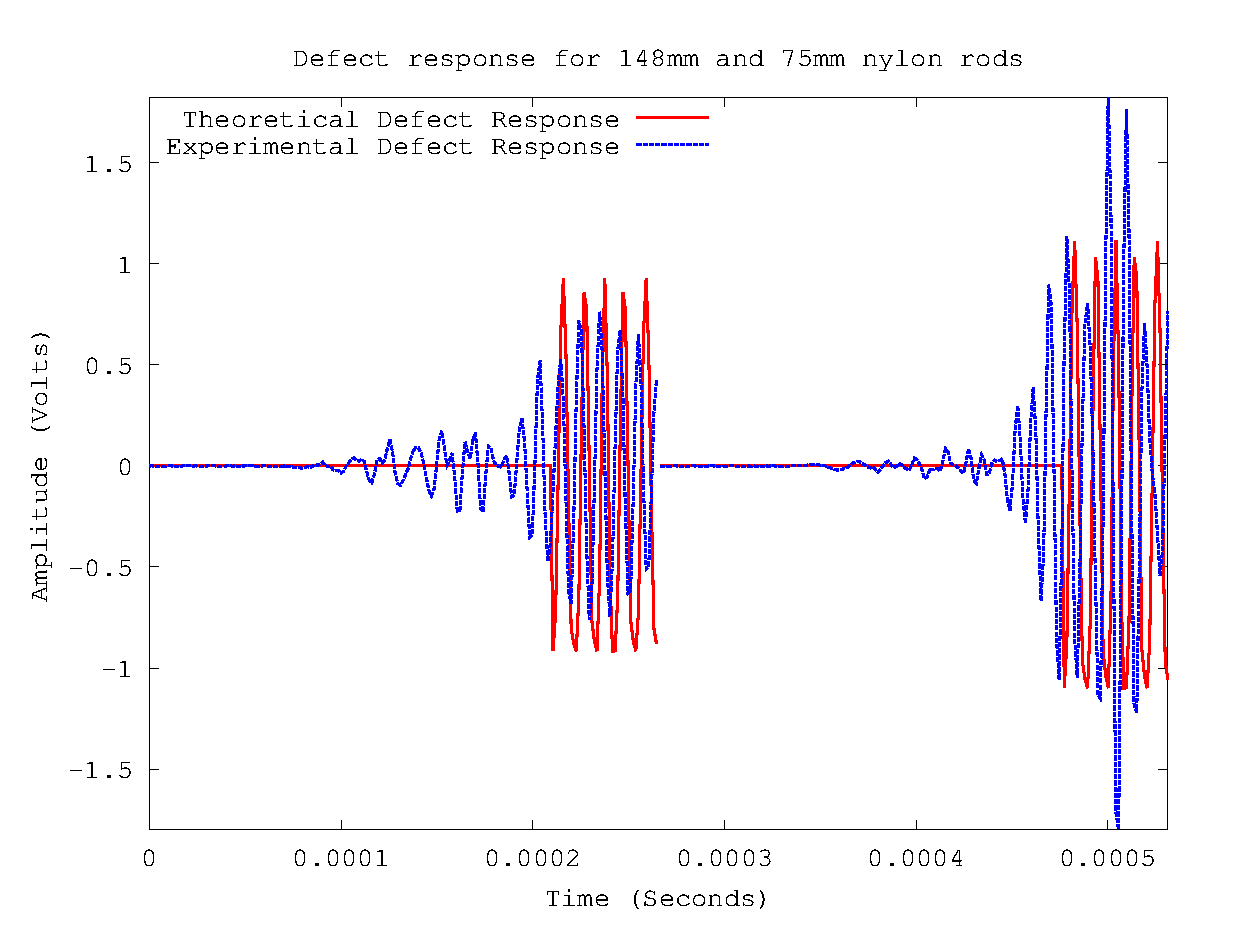
\includegraphics[width=9.7cm,height=5.75cm]{nylon-2-4_Iter_th_exp.eps}}
\subfigure[Theory vs Experiment, 105mm and 75mm nylon rods]
{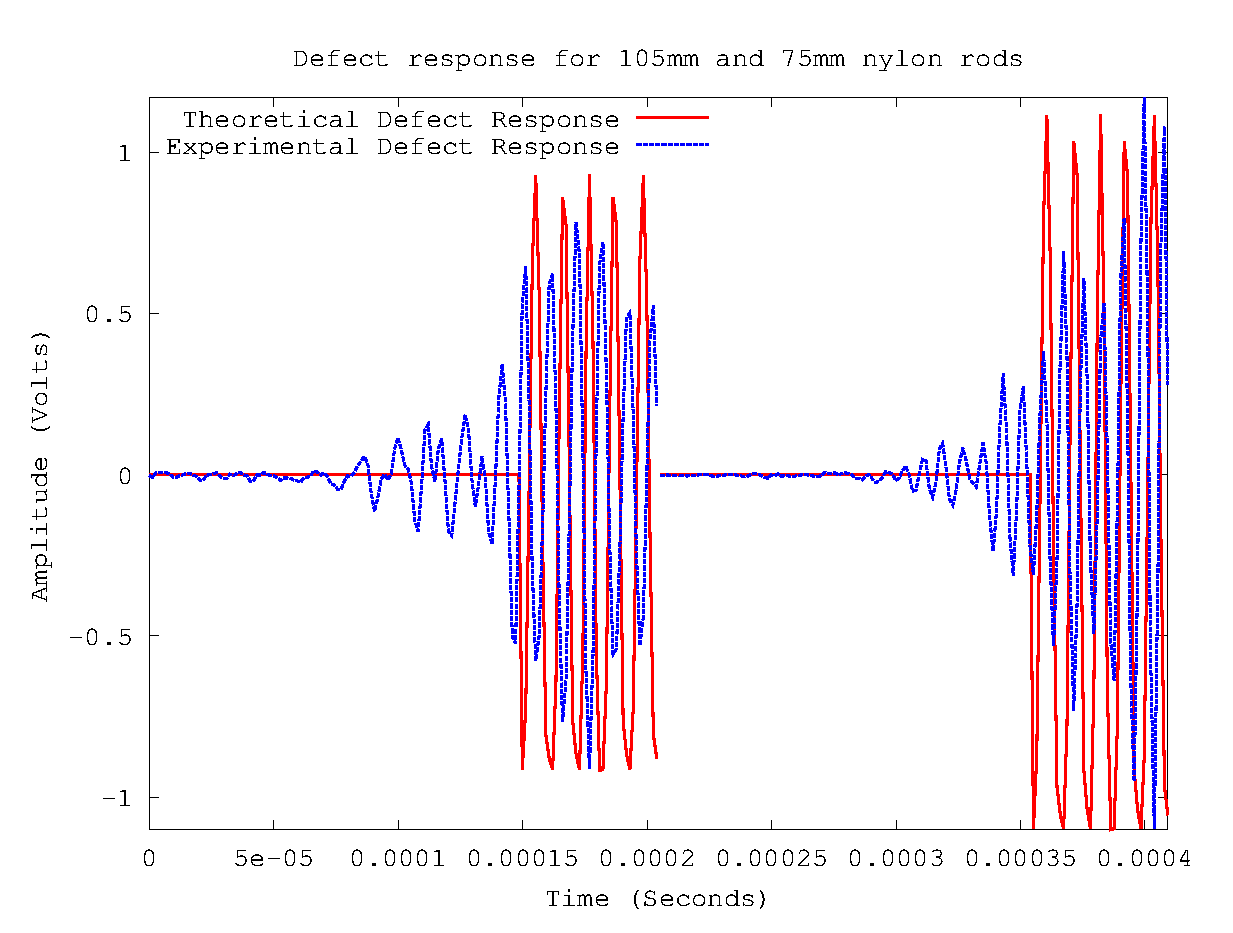
\includegraphics[width=9.7cm,height=5.75cm]{nylon-3-4_Iter_th_exp.eps}}
\end{subfigmatrix}

   \caption[all]
%>>>> use \label inside caption to get Fig. number with \ref{}
   { \label{nylonThExp}
Nylon rod experimental results for the response seen at the defect PZT plotted with the theoretical calculations for the response. The results were plotted for each of the three nylon rod tests. Similar to what was seen in the steel rod results (although worse),  there was a decent match between theory and experiment. The differences could be accounted for by a lack of dispersion and dissipation in the predicted records.
 }
 \end{figure}

By looking at the gain plots of the defect PZT, the overall effectiveness of the iterative time reversal algorithm for the nylon rods was measured (Figures \ref{nylonExp1}-\ref{nylonExp3}). The results for the amplitude gain vs iteration were seen to be better than that achieved with the steel rod tests. In the steel rod tests gains closer to 2 were recorded whereas in the nylon rod tests gains closer to 3 were achieved. This was consistent with studies performed by Fink et al (2000) which suggested that the time reversal algorithm works better in materials with higher dispersion rates. It was also seen in the nylon rod tests that the final wave recorded at the defect PZT was of much greater amplitude than that of the initial wave seen at the defect PZT (Figures \ref{nylonExp1}-\ref{nylonExp3}).

 \begin{figure}
\begin{subfigmatrix}{3}
\subfigure[Defect Response Initial Iteration, 148mm and 105mm nylon rods]
{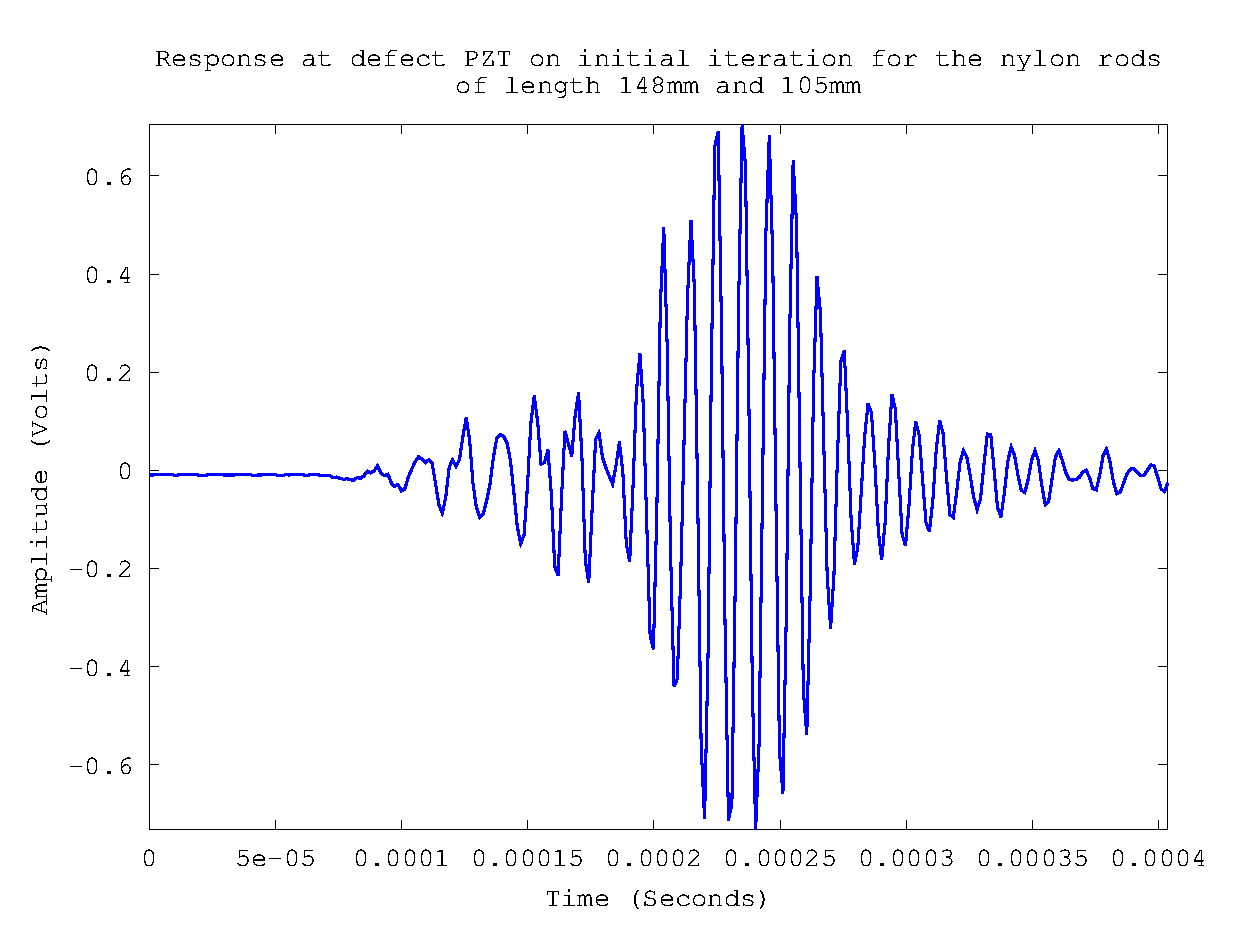
\includegraphics[width=9.7cm,height=5.75cm]{nylon-2-3_Initial.eps}}
\subfigure[Defect Response 150th Iteration, 148mm and 105mm nylon rods]
{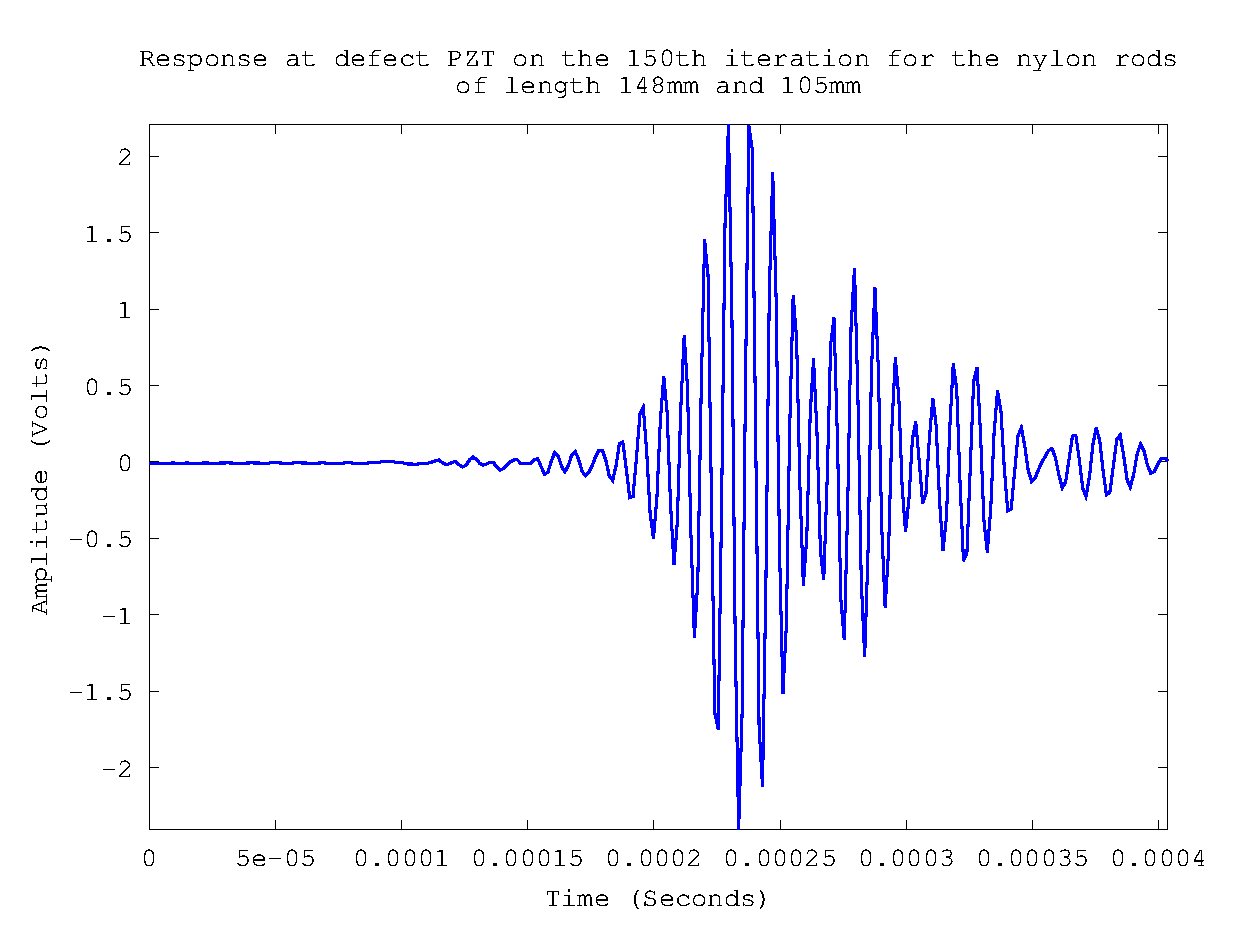
\includegraphics[width=9.7cm,height=5.75cm]{nylon-2-3_Final.eps}}
\subfigure[Defect Amplitude Gain, 148mm and 105mm nylon rods]
{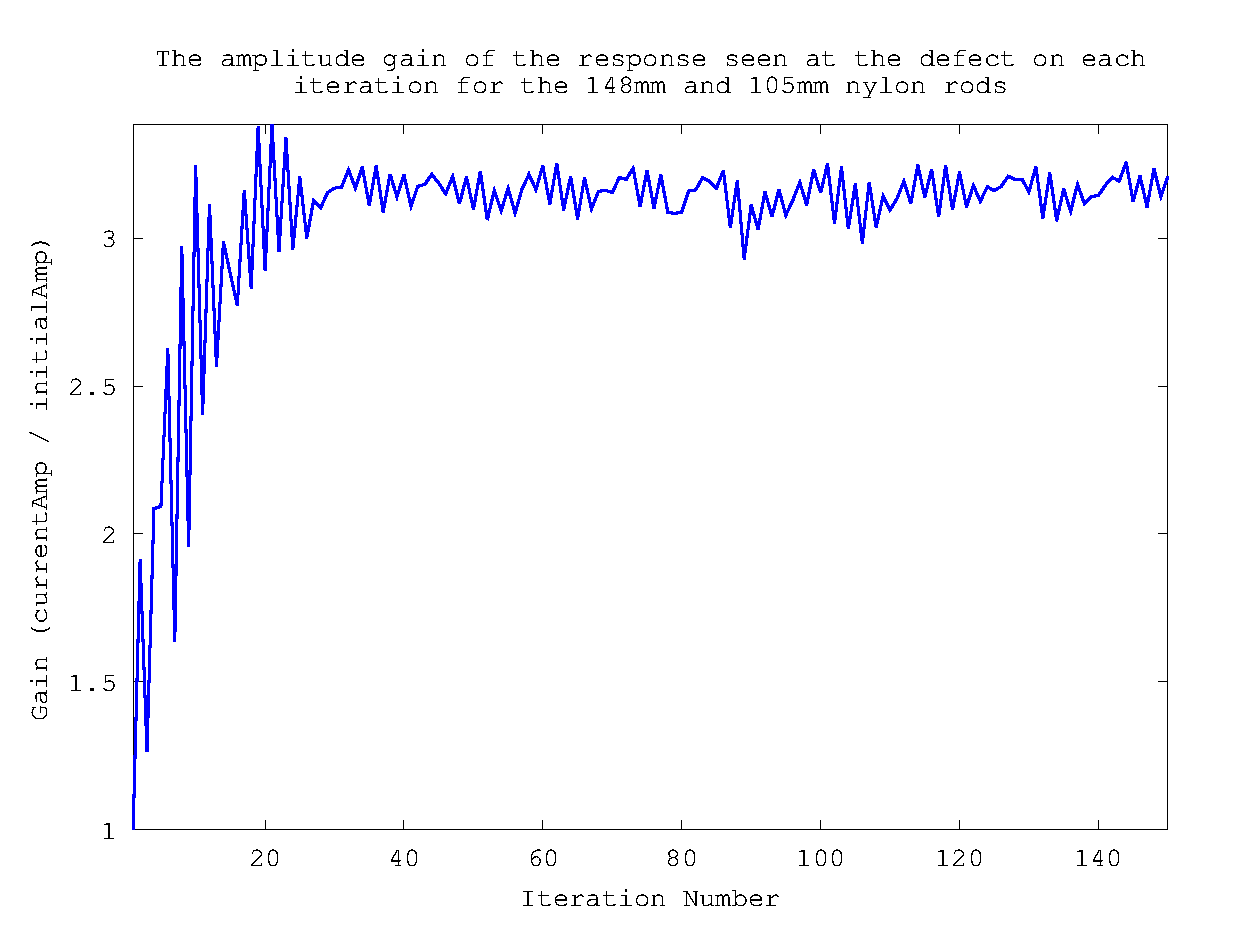
\includegraphics[width=9.7cm,height=5.75cm]{nylon-2-3_iterationVsGain.eps}}
\end{subfigmatrix}

   \caption[all]
%>>>> use \label inside caption to get Fig. number with \ref{}
   { \label{nylonExp1}
   a) First wave seen at the defect on the initial iteration for the 148mm and 105mm nylon rod test.; b) Wave recorded at the defect after 150 iterations. The final wave more than tripled in amplitude from the first wave; c) Plot of the amplitude gain that was achieved at the defect for each iteration of the time reversal algorithm. The gain leveled out around 3.
 }
\end{figure}

 \begin{figure}
\begin{subfigmatrix}{3}
\subfigure[Defect Response Initial Iteration, 148mm and 75mm nylon rods]
{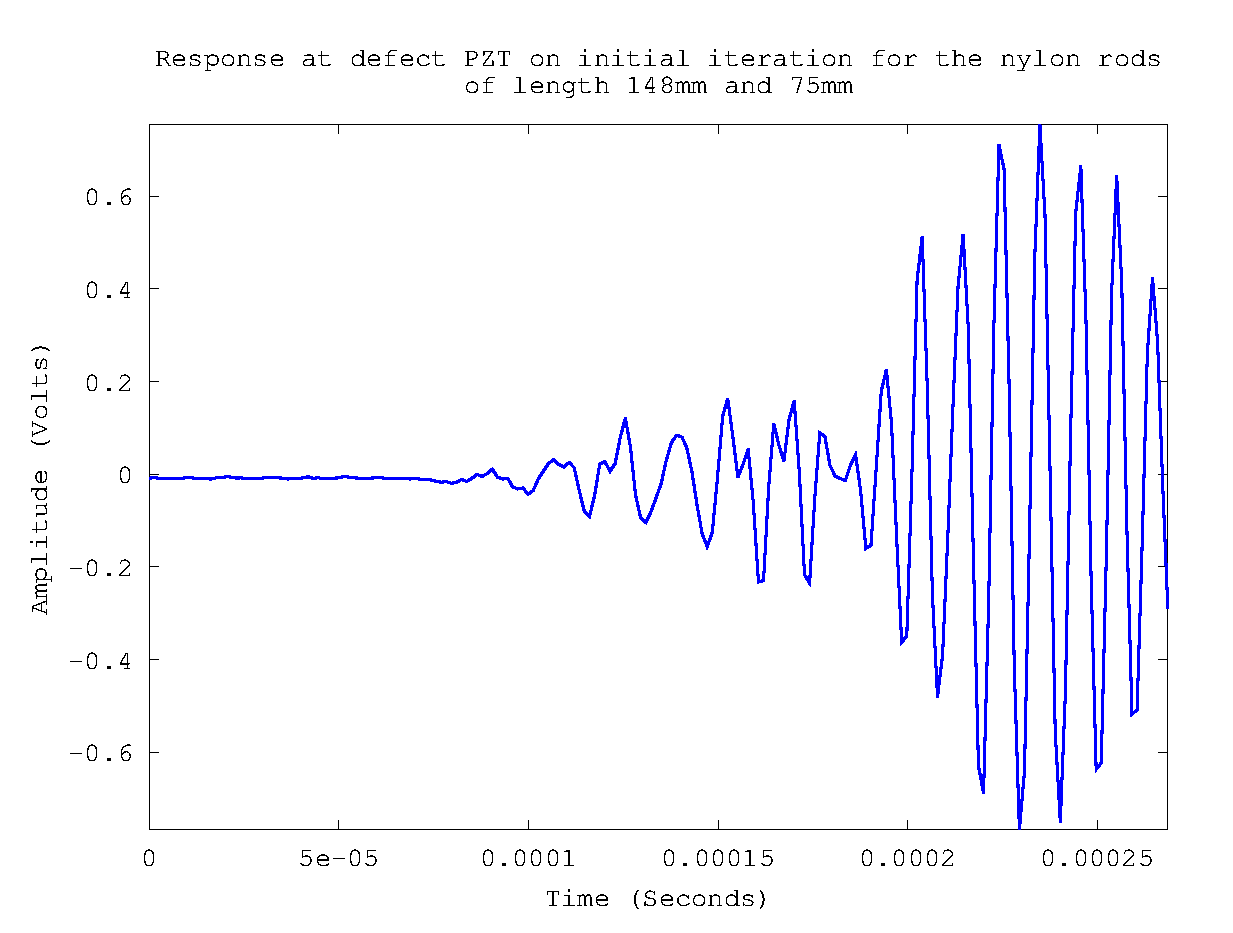
\includegraphics[width=9.7cm,height=5.75cm]{nylon-2-4_Initial.eps}}
\subfigure[Defect Response 150th Iteration, 148mm and 75mm nylon rods]
{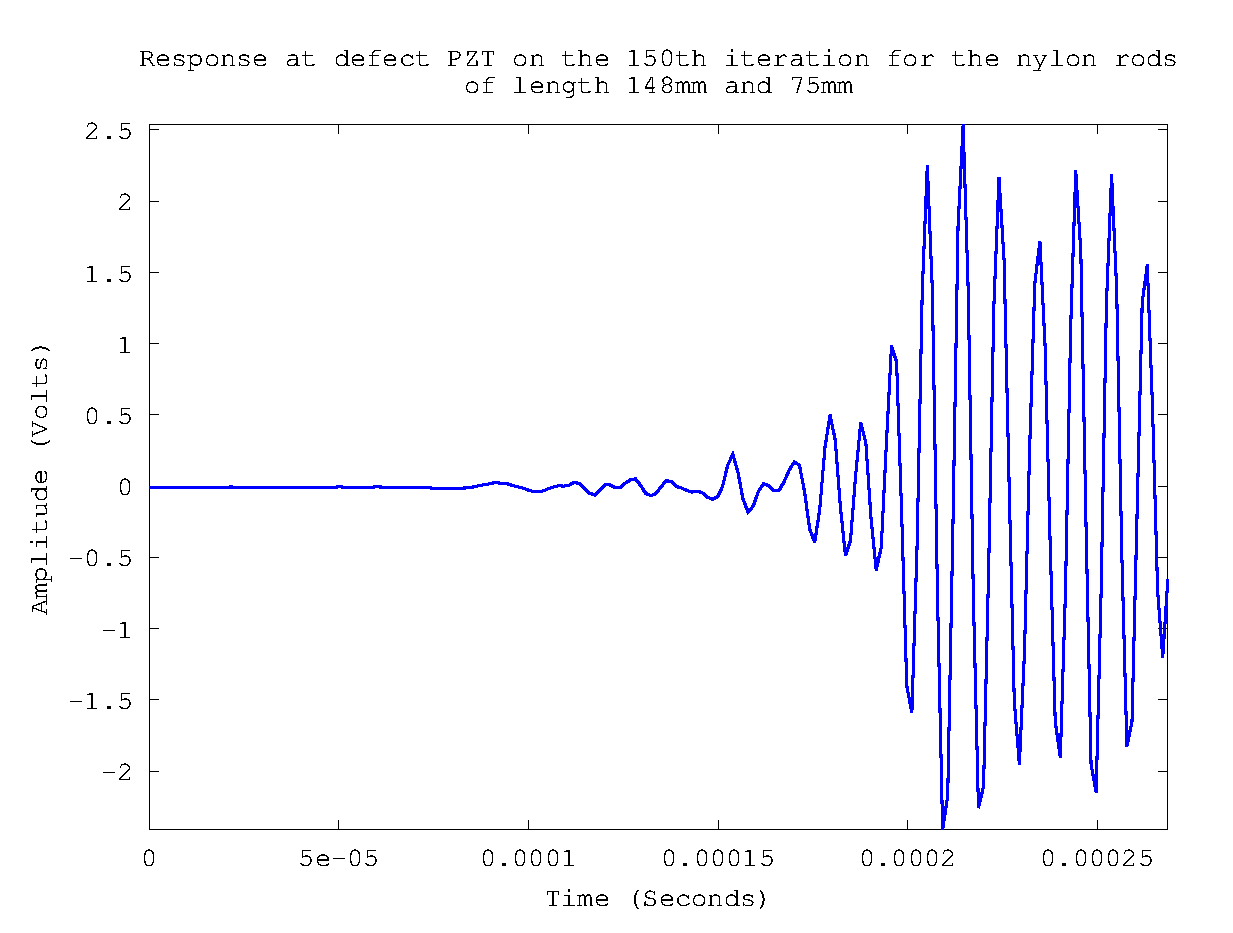
\includegraphics[width=9.7cm,height=5.75cm]{nylon-2-4_Final.eps}}
\subfigure[Defect Amplitude Gain, 148mm and 75mm nylon rods]
{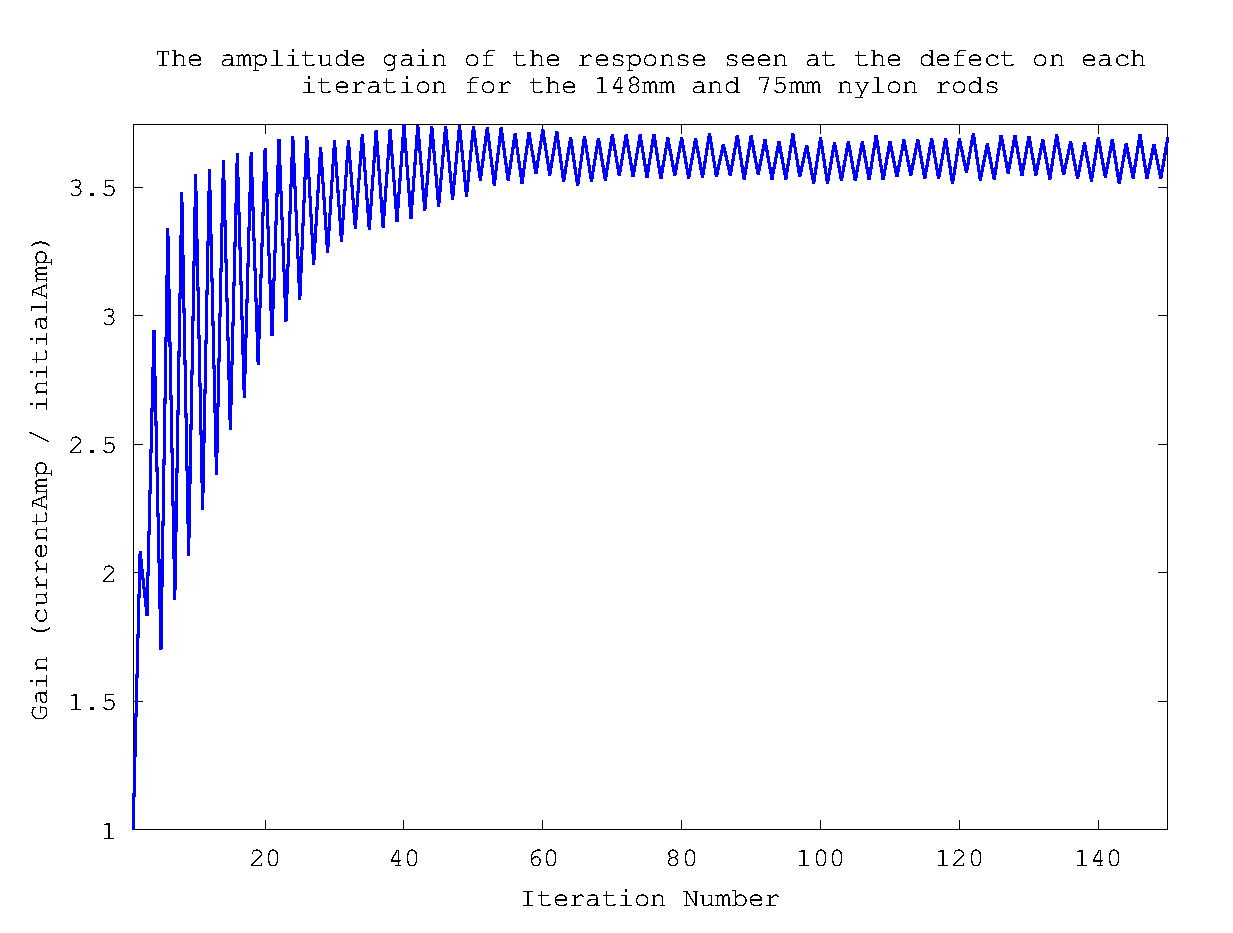
\includegraphics[width=9.7cm,height=5.75cm]{nylon-2-4_iterationVsGain.eps}}
\end{subfigmatrix}

   \caption[all]
%>>>> use \label inside caption to get Fig. number with \ref{}
   { \label{nylonExp2}
   a) First wave seen at the defect on the initial iteration for the 148mm and 75mm nylon rod test.; b) Wave recorded at the defect after 150 iterations. Again, the response seen at the defect has tripled; c) Plot of the amplitude gain that is achieved at the defect for each iteration of the time reversal algorithm, with a convergence gain of a little over 3 which was actually reached by about the 25th iteration as seen in other tests.
 }
\end{figure}

 \begin{figure}
\begin{subfigmatrix}{3}
\subfigure[Defect Response Initial Iteration, 105mm and 75mm nylon rods]
{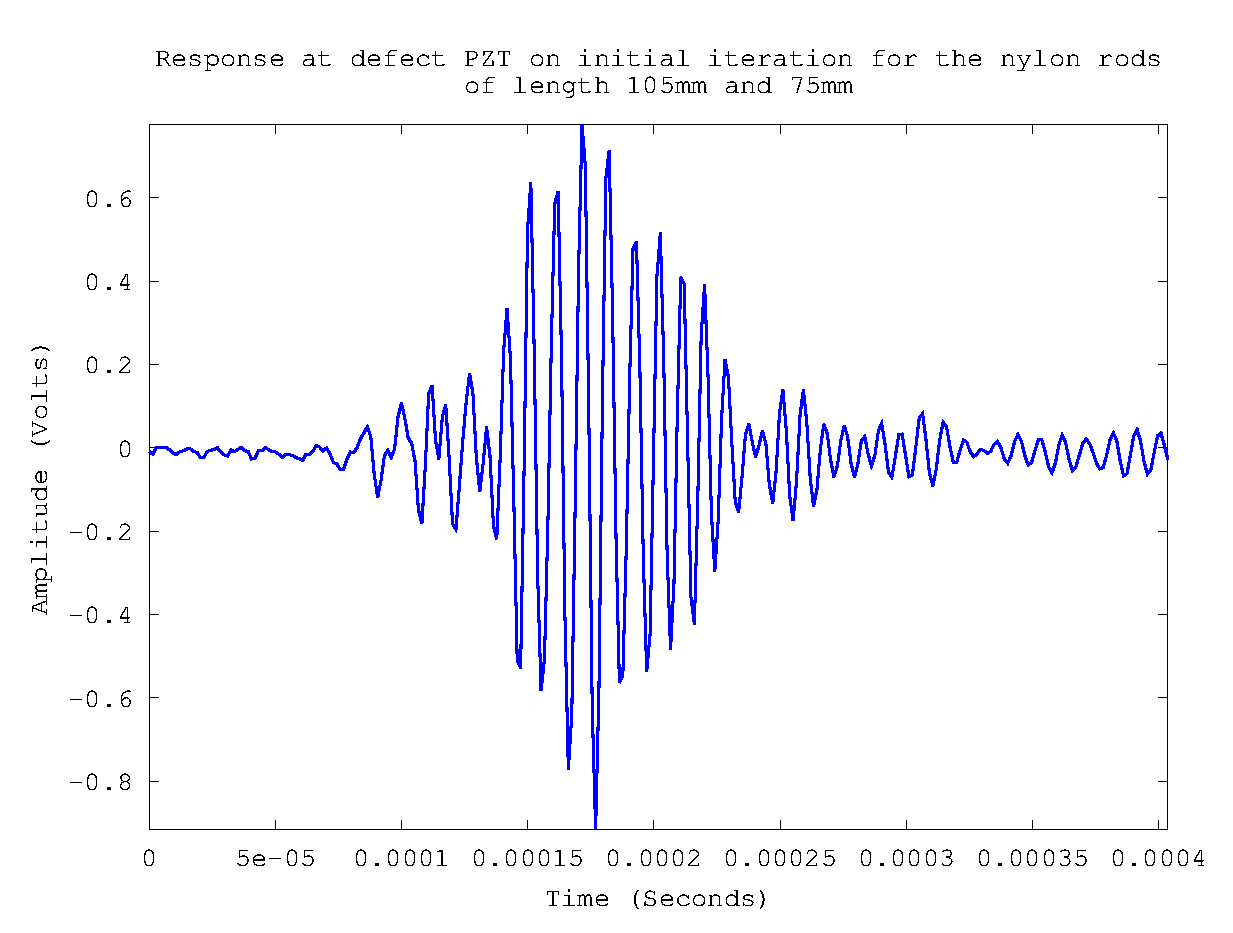
\includegraphics[width=9.7cm,height=5.75cm]{nylon-3-4_Initial.eps}}
\subfigure[Defect Response 150th Iteration, 105mm and 75mm nylon rods]
{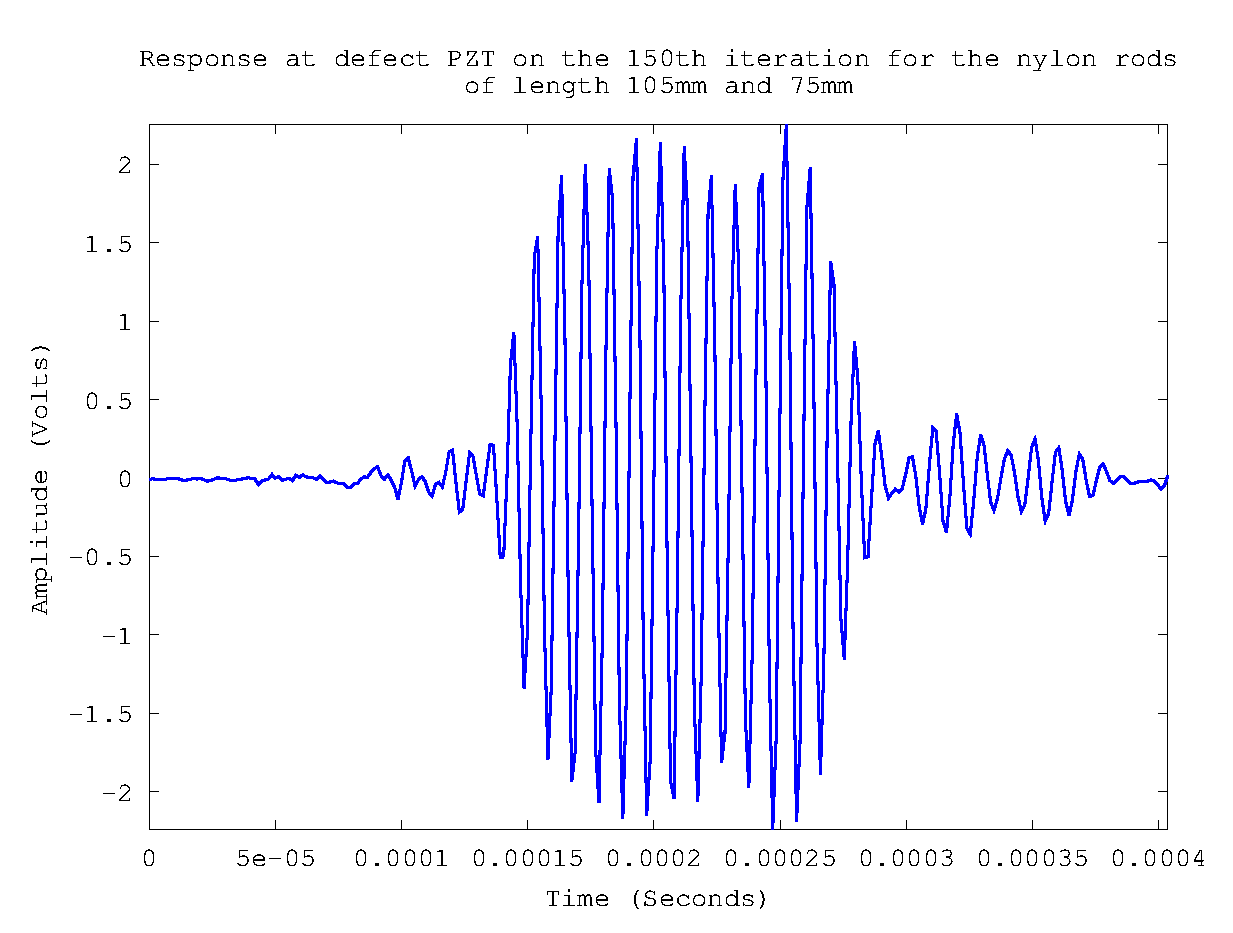
\includegraphics[width=9.7cm,height=5.75cm]{nylon-3-4_Final.eps}}
\subfigure[Defect Amplitude Gain, 105mm and 75mm nylon rods]
{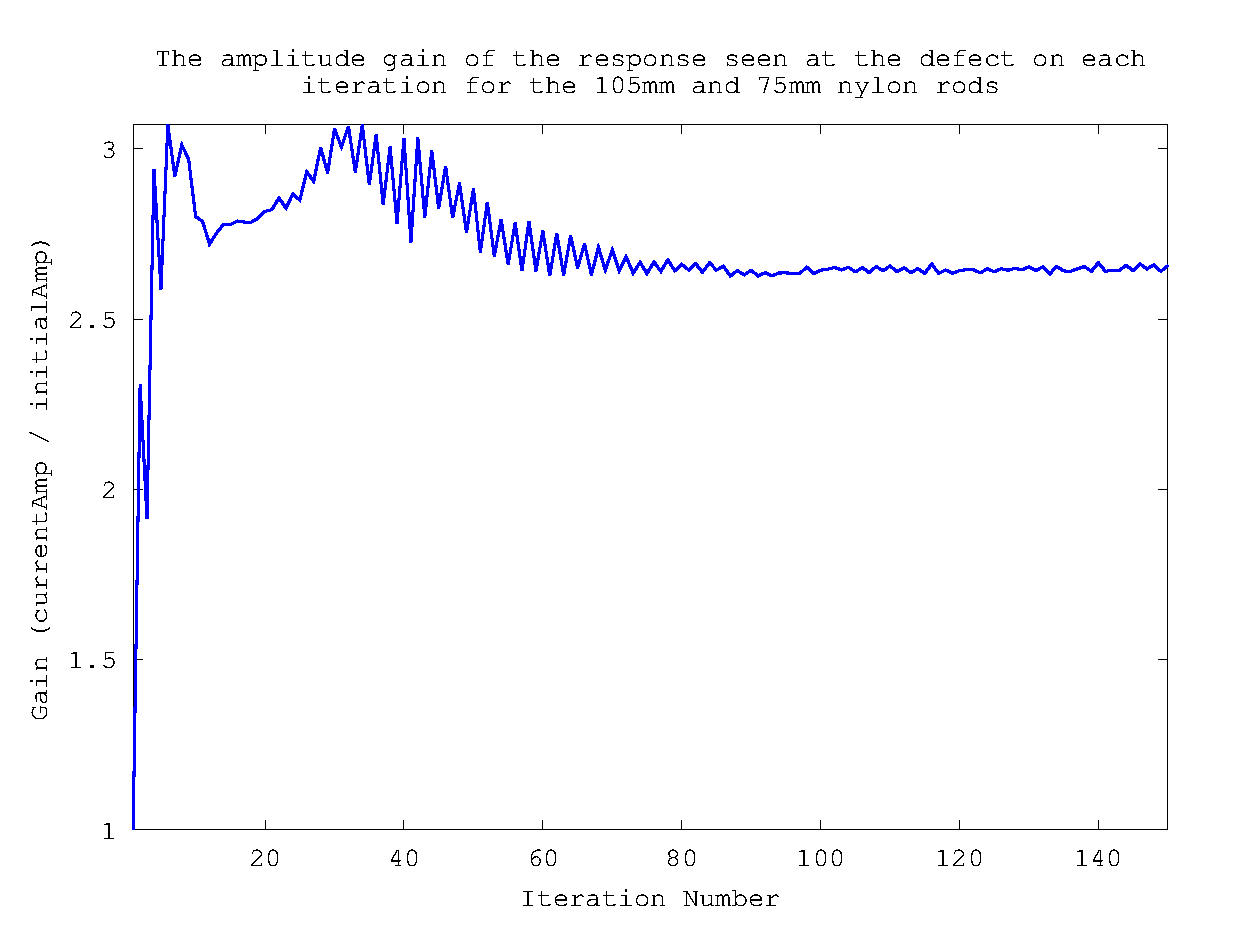
\includegraphics[width=9.7cm,height=5.75cm]{nylon-3-4_iterationVsGain.eps}}
\end{subfigmatrix}

   \caption[all]
%>>>> use \label inside caption to get Fig. number with \ref{}
   { \label{nylonExp3}
   a) First wave seen at the defect on the initial iteration for the 105mm and 75mm nylon rod test.; b) Wave recorded at the defect after 150 iterations. c) Plot of the amplitude gain that was achieved at the defect for each iteration of the time reversal algorithm, with a convergence gain of about 2.75. This test was a good example of the convergence gain being lower than the max gain that was seen and suggests that the algorithm could be further improved.
 }
\end{figure}


\section{CONCLUSION}
\label{sect:concl}

The idea of autonomic defect healing has received considerable
attention in the last decade or so, and a number of approaches
have evolved around choosing the correct chemistries for the
parent materials and/or catalysts that would enable crack sealing
and strengthening when acted upon by certain trigger mechanisms.
In environments where the forces causing damage occur concurrently
with the healing processes, it would be advantageous to consider
methods to accelerate the healing rate so as to restrict the net
damage to the structure.  

Time reversal mirrors and focusing of multi-tone stress waves in 1-dimensional
finite domains, such as may be encountered in tubular or
shaft-like structures, were investigated here. In the time reversal mirror studies, a reasonable degree of amplification was found at the defect using iterative
time reversal play back for both a largely non-dispersive
1-dimensional propagation case in steel rods and a more
dispersive and dissipative propagation case in nylon rods. Gains of over 2 for the steel rod experiments and gains of over 3 for the nylon rod tests were achieved. The higher gains with the nylon versus steel were consistent with the theory that time reversal works better in materials with higher dispersion. Further improvements could be made to the algorithm so that the convergence gain is the optimal gain that is available.

1-dimensional epoxy curing experiments with the introduction of acoustic energy have been reported elsewhere \cite{fehrman}.
It would be worthwhile to develop this investigation further, to
2-dimensional epoxy domains with multiple transducers on the sides
and an embedded transducer simulating a crack.  In addition, more
direct acoustic stimulation methods could be used in 2 dimensions
with excitation via attached ultrasonic horns in a slow-curing
epoxy, while tracking the healing progress with sequenced
microstructure measurements on different samples through the
different stages of curing.  It would be particularly interesting
to combine time reversal mirrors with crack healing in polymer
resin dog-bone samples with continual observations of mechanical
properties.  The 1-dimensional implementation studied here could
be of relevance to nondestructive defect detection in molding or
casting of circular rods.

\section*{ACKNOWLEDGEMENT}

We are grateful to the Air Force Research Laboratory, Space
Vehicles Directorate (AFRL/RV) for their support of this work.
Particular thanks are due to Dr. Jeffry Welsh and Mr. Jeremy Banik
at AFRL/RV and Dr. Chris Jenkins at Montana State University for
their insights and suggestions. We would also like to thank Alexander Cushman for all of his work on this project.


\bibliographystyle{unsrt}
\bibliography{references_time}

\end{document}
